\documentclass[letter,12pt]{article}
\usepackage[letterpaper,right=1.25in,left=1.25in,top=1in,bottom=1in]{geometry}
\usepackage{setspace}

\usepackage[utf8]{inputenc}   % allows input of special characters from keyboard (input encoding)
\usepackage[T1]{fontenc}      % what fonts to use when printing characters       (output encoding)
\usepackage{amsmath}          % facilitates writing math formulas and improves the typographical quality of their output
\usepackage[hyphens]{url}     % adds line breaks to long urls
\usepackage[pdftex]{graphicx} % enhanced support for graphics
\usepackage{tikz}             % Easier syntax to draw pgf files (invokes pgf automatically)
\usetikzlibrary{arrows}

\usepackage{mathptmx}           % set font type to Times
\usepackage[scaled=.90]{helvet} % set font type to Times (Helvetica for some special characters)
\usepackage{courier}            % set font type to Times (Courier for other special characters)

\usepackage[longnamesfirst, sort]{natbib}\bibpunct[]{(}{)}{,}{a}{}{;} % handles biblio and references 

\usepackage{rotating}         % sideway tables and figures that take a full page
\usepackage{caption}          % allows multipage figures and tables with same caption (\ContinuedFloat)

\usepackage{dcolumn}          % needed for apsrtable and stargazer tables from R to compile
\usepackage{arydshln}         % dashed lines in tables (hdashline, cdashline{3-4}, 
                              %see http://tex.stackexchange.com/questions/20140/can-a-table-include-a-horizontal-dashed-line)
                              % must be loaded AFTER dcolumn, 
                              %see http://tex.stackexchange.com/questions/12672/which-tabular-packages-do-which-tasks-and-which-packages-conflict


\newcommand{\mc}{\multicolumn}

%% TO ADD NOTES IN TEXT, PUT % BEFORE THE ONE YOU WANT DISBALED
%\usepackage[disable]{todonotes}                            % notes not showed
\usepackage[colorinlistoftodos, textsize=small]{todonotes} % show notes
\newcommand{\emm}[1]{\todo[color=red!15, inline]{\textbf{Eric:} #1}}
\newcommand{\vp}[1]{\todo[color=green!15, inline]{\textbf{Vale:} #1}}
\newcommand{\ges}[1]{\todo[color=blue!15, inline]{\textbf{Ges:} #1}}

% agradecimientos
% Sebastián Soto Velasco, ex-director jurídico de del ministerio secretaría general de la presidencia
% Roberto Bustos, Secretario de la Comisión de Hacienda del Senado
% Alvaro Villarroel, staff Comisión de Hacienda del Senado
% Tercer staff de Comisión de Hacienda del Senado
% Dip. Patricio Vallespín
% Dip. 1er vice-presidente de la Cámara de Diputados

% [28-8-2017] improvements for logit
% a. drop member bills or analyze separately
% b  control whether or not bill was reported: this is gatekeeping
% b.1  analyze this as a separate DV
% b.2  use a conditional model: not reported are not same type
%    |    | U   | ~U  |
%    |----+-----+-----|
%    | G  | g_u | g_s |
%    | ~G | u   | s   |
%    |----+-----+-----|
 

\begin{document}

\title{Restrictive rules in the Chilean Cámara: Fighting floor amendments with urgency authority\thanks{Paper read at the 2017 annual meeting of the American Political Science Association, San Francisco, CA, Sept.~1, 2017. The authors are grateful to Roberto Bustos, Alvaro Villarroel, and the staff of the Senate's Hacienda committee, and especially to Sebastián Soto Velasco for help understanding urgency authority; to Deputy Patricio Vallespín for making calls to schedule interviews with congressional personnel; to Ernesto Calvo and José Antonio Cheibub for comments and critiques to previous incarnations of the paper. Eric Magar acknowledges financial support from the Asociación Mexicana de Cultura A.C.\ and CONACYT's Sistema Nacional de Investigadores. Valeria Palanza acknowledges support from Proyecto Fondecyt No. 1140974, and from the Millennium Nucleus for the Study of Stateness and Democracy in Latin America, Project \#NS100014. The authors bear sole responsibility for mistakes and shortcomings in the study.}}
\author{Eric Magar \\ ITAM \and
        Valeria Palanza \\ Univ.\ Católica de Chile \and  
        Gisela Sin \\ Univ.\ of Illinois, Urbana-Champaign 
}
\date{\today}
\maketitle

%\begin{center} \textbf{$\rightarrow$~~Preliminary draft~~$\leftarrow$} \\ (please inquire for new version, \small{\url{emagar@itam.mx}})  \end{center}

\begin{abstract}
\noindent Among the formidable proactive legislative powers of Chile's president is urgency authority. Lawmakers face a short deadline to discuss and vote bills declared urgent. Extant research has shown that most executive proposals become urgent at some stage, that urgency correlates with the odds of passage, but found little evidence that it speeds consideration of the president's agenda in Congress. This paper underscores a procedural distinction of this institution that scholars have overlooked: the floor considers urgent bills under \emph{restrictive rules}, giving presidents the ability to shield committee reports from floor amendments. Hypotheses derived from a formal model of restrictive rules are tested with data from the 1998--2014 period. We provide significant evidence that urgency messages associate with the type of restrictive rule correlates found in the U.S.
\end{abstract}

% comentarios de Calvo
%Comentarios a Magar: Presidential obstruction of the agenda in Chile’s Congress
%Buenísimo el paper. Siempre me pareció muy interesante el tema de las urgencias y no existen análisis sistemáticos de estos procesos. Tengo muchas ganas de ver el libro completo una vez que esté terminado. 
%En términos generales me gusta mucho la perspectiva y el modelo es interesante. El juego está descripto con poco detalle (supongo que eso viene en otros capítulos) así que la presentación de la Figura 2 y su discusión en las páginas 10 y 11 siguen siendo un poco crípticos. La intuición se entiende, pero el hecho de que en distintos sistemas k y o toman distintos valores y producen distintos equilibrios necesita más fundamentación (de nuevo, asumo que eso viene de capítulos anteriores del libro). 
%El capítulo preguntando porque los legisladores toman en consideración las “urgencias” cuando a diferencia de Brasil o Uruguay no existe un mecanismo de sanción si ellos “shirk”. No tenemos respuesta a lo largo del capítulo y mi impresión es que se necesita un poco mas de data cualitativa (algunas entrevistas o discusiones de diarios de sesiones) que digan porque los legisladores atienden al pedido del presidente. Esto quizá afecte como pensas el modelo de la Figura 2 y te convendría resolverlo antes de cerrar el capítulo.
%Mi preocupación principal está en la forma en que usas la data y como estimas el modelo. Las “urgencias” son un mecanismo para presionar al Congreso para que actúe y, por tanto, tienen que ser modelados con una función de tiempo. Lo más natural para mí sería utilizar un “mixture” model que mide al mismo tiempo la “tasa” de aprobación y el “tiempo” de aprobación (te anexo un artículo en el cual hacemos esto para el caso de Uruguay con Chasquetti). Entiendo que las “urgencias” son una forma de presionar al Congreso para resolver favorablemente, pero la discusión sobre el “scheduling” del plenario también refiere al problema del costo de oportunidad de tratar los proyectos del Presidente en lugar de los proyectos de los legisladores. Sin embargo, todos los Congresos tienen mecanismos para permitir que los “pet projects” sean aprobados cuando hay tiempos limitados en el plenario. En Brasil las comisiones pueden dar aprobación final a una gran cantidad de projectos (“terminativa”) para evitar consumir el tiempo del plenario. En Argentina el artículo 133 del reglamento permite votar en paquete proyectos que tienen dictamen de comisión y no tienen objeciones ni enmiendas. Por lo tanto, existen cambios en las reglas que les permiten a los legisladores “circunvent” las restricciones de tiempo del plenario. Para mi es necesario modelar el éxito relativo y el tiempo de aprobación para ver que es lo que están haciendo las urgencias.
%Esto también quiere decir que el modelo de estimación debería ser al nivel de proyecto de ley y no un OLS con sumas de instancias. Sino me equivoco tenes toda esa data, el N es mas grande y además te permite combinar data a nivel de proyecto, de legislador y de Congreso. Así que a mi juicio conviene cambiar la estrategia de estimación. 
%Por lo demás, me parece un excelente artículo y me muero de ganas de ver el libro.
%Abrazo. E.  


\onehalfspacing

\section{Introduction}

\noindent The prerogative to declare bills urgent gives the president power to interfere with congress' voting schedule. Presidents with such power can impose legislators with a deadline to discuss and vote legislation by simply designating a bill ``urgent''. Seen against presidential systems like the U.S., where an impatient president has no formal resources to pressure legislators to act on stagnant legislation, urgency authority seems contradictory to classic notions of separation of powers. In Federalist 47, Madison argues that ``The magistrate in whom the whole executive power resides cannot of himself make a law, though he can put a negative on every law'' \citep{madison.47}.

\ges{Not happy about this quote yet, but I think is more appropriate than the previous one.  We need something about separation of powers.
    The Framers warn against expediting lawmaking and arresting deliberation. ``In the legislature promptitude of decision is oftener an evil than a benefit'' \citep{hamilton70.1788}.
    Within this view presidents can veto bills, preventing them from becoming law, but cannot force legislators to act on specific measures.}

% federalist 70
% Upon the principles of a free government, inconveniences from the source just mentioned [collective actors] must necessarily be submitted to in the formation of the legislature; but it is unneccessary, and therefore unwise, to introduce them into the constitution of the executive. It is here too that they may be most pernicious. In the legislature promptitude of decision is oftener an evil than a benefit. The differences of opinion and the jarring of parties in that department of the government, though they may sometimes obstruct salutary plans, yet often promote deliberation and circumspection, and serve to check the excesses of the majority. When a resolution too is once taken, the opposition must be at an end. That resolution is a law, and resistance to it is punishable. --> EMM la urgencia opera contra esta delibaración benévola...
% federalist 47 "The magistrate in whom the whole executive power resides cannot of himself make a law, though he can put a negative on every law" 

Yet, five constitutions of the Americas give presidents such authority: Brazil, Chile, Colombia, Mexico, and Uruguay \citep{morgenstern.2002b}. In Brazil, the president can declare any executive-initiated bill urgent at any time. The assembly must act on urgent legislation within forty five days, else the bill in question takes precedence over all other legislative business. In Colombia, urgent bills go to the top of the voting schedule immediately, and all activity on the floor stops until legislators vote on the bill. In Uruguay, legislators must act within a pre-specified, short period of time, as failure to do so converts the urgent bill into law. \footnote{Although three-fifths of the membership of either chamber can remove the bill's urgent status.}  In Mexico, the president can propose up to two urgent bills at the start of each biannual ordinary period, which must be scheduled for floor consideration within 30 days.\footnote{Constitutional articles vesting this authority are the following: Brazil articles 62 and 64; Chile article 74; Colombia article 163; Mexico article 71; and Uruguay article 168.7.}

\emm{How does this compare with special (extra-ordinary) sessions? Some presidents can summon legislators to a special session to discuss, exclusively, a specific bill defined ex-ante. Limits? If few, might resemble urgency authority... Check.}
\vp{WILL LOOK INTO THIS}
\ges{Little, if any connection.}

In the United States, \citet{howell.moe.Relic2016} \todo{Find book, change quote (from CNN)} argue that in order to have an effective government, reform needs to put the president at the center of the legislative process by giving him precisely urgency powers: a ``constitutional amendment that grants presidents universal `fast track' authority... Presidents would craft policy proposals---which are likely to be far more coherent, well-integrated, and effective than anything Congress would design---and Congress would be required to vote up or down on those proposals, within a specified period of time and on a majority-rule basis''. 

The key element in these rules is the reversion point when Congress fails to act on an urgent measure: the whole legislative process comes to a halt (as in the case of Brazil and Colombia), the bill becomes a law (as in the case of Uruguay), or provisions of the Constitution are violated (under the Howell-Moe proposal for the U.S.). Thus, by institutional design, the president has an effective avenue to influence the congressional agenda: s/he can force Congress to debate and vote on a bill.

In Chile, however, failure to act on an urgent bill does not carry any kind of trigger effect. The legislative process does not stop, and bills do not become law immediately. There are no formal consequences when legislators do not consider a bill under the period of time specified in the urgency. Indeed, legislators can ignore the president's request for action.  Scholars have speculated that the value of the urgency authority lies in its signaling capacity. Quoting a former legal chief of staff at the Presidency, \citet{berrios.gamboa.fiscChile.2006} describe one month notices as ``merely symbolic, exerting no real pressure on Congress'' (p.117). Likewise, \citet{aleman.navia.UrgChi.2009} see degrees of urgency as ``signals of presidential attention'' (p.~404). The assembly may face political costs by ignoring or rejecting salient proposals. In his study of the urgency prerogative in Chile's first post-transition administration,  \citet{siavelis.2002}  revealed the high frequency with which urgency messages were issued by President Aylwin. He also found mixed evidence on whether proposals marked urgent had a more expedited legislative process and an improved likelihood of passage. 

Our argument builds on the existing literature, but takes on a very different position.  In short, we claim that urgency authority is neither a signal nor an agenda setting tool, but instead a mechanism that enhances cooperation between the executive and his party or coalition in Congress. We find that the literature has largely ignored an important consequence of this rule: when bills are labeled urgent, they cannot be modified on the floor. Urgent bills are proposals that come to the floor with a close rule:  legislators have to vote it up or down, with no possibility to introduce amendments.  Under this prerogative, the bill that emerges from committee is identical to the bill that is enacted. Urgency protects the commitments agreed to in committee as they cannot be undone later on on the floor. 

The interesting element in Chile is that it is the president who decides whether a bill proceeds to the floor with a close rule, or whether it will be open for amendments. This means that, unlike the U.S., where committee members negotiate with the leadership and the Rules Committee to receive close rules towards floor consideration, in Chile committee members negotiate with the president to receive that label. In other words, in Chile the president takes on the role of the Rules Committee. 

This unique presidential role opens the door for multiple strategies both for the committee and the president regarding the conditions under which they will push for a bill to receive the urgency label. 

%We claim that the poor signal given by bills designated urgent in Chile may bear relation to selection bias. Strategic presidents are likely to target bills that differ from the rest in important ways, so that the set of bills receiving urgent status is not random. Right censoring may also be an obstacle. A more fundamental problem is institutional indeterminacy. \citet{berrios.gamboa.fiscChile.2006} warn against overstating the Chilean urgency authority's importance, as non-compliance entails no penalty for Congress. %---unlike the Brazilian, Colombian, and Uruguayan variants.
%This paper argues that the effects of urgency authority are procedural. Proposals the president declares urgent in Chile are considered under restrictive rules by the chamber's plenary. If the rationale is expediting the legislative process, one key consequence is to effectively shield committee reports from amendments by the plenary.

\vp{Me sigue pareciendo que está faltando una sección que discuta la literatura sobre Chile, sea en la sección 2, antes de cerrar la 1, o una nueva sección 1,5 por decir algo. Yo puedo escribir un par de páginas en ese espíritu post-APSA, y eso engancharía con lo que Ges se comprometió a escribir pre-APSA sobre el puzzle. INCLUIR a Alemán y Navia, y ver qué más}

The paper proceeds as follows. Section 2 describes the urgency process in Chile in more detail and presents the data. We elaborate on urgency degrees, a distinction of central importance to the study of this institution in Chile, offering our interpretation of the urgency authority as a restrictive rule. Schematizing the sequence of committee reports and plenary readings shows that it is much harder to introduce plenary amendments to urgent than non-urgent bills. Section 3 extends a simple model of restrictive rules from the U.S.\ to the Chilean Congress. The spatial model highlights the logic behind the procedural choice: when the executive anticipates that a palatable committee report is vulnerable to floor amendments, declaring it urgent imposes a take-it-or-leave-it vote on the floor. We derive testable hypotheses. Section 4 tests some of them. Examination of all bills in the 1998--2014 period through multivaiate analysis in search of urgency authority predictors shows that, other features constant, bills reported by committees chaired by the president's party/coalition (our measure of preference similarity between the president and the committee chair, driving some theoretical results) associates significantly with urgency messages. Section 5 concludes. 

\emm{Post APSA: I believe that the urgency dummies are coded for both the Camara and the Senate, while controls in the empirical model are just for the Camara---hence my application of the argument to the lower chamber only. We need to somehow either filter Senate urgencias from the indicators, or add upper chamber controls in order to generalize the model to the Congress.} 

\section{Urgent legislation and urgency degrees}

As part of a literature that highlights the extraordinary legislative influence of presidents in Latin America, emphasis has been placed on the Chilean president's capacity to initiate legislation, to veto bills at their final stage, and to propose amendments at different times. Less attention has been devoted to the influence gained by the president when s/he can declare certain bills urgent and affect how congress deals with its agenda.  We collected original data to investigate urgency authority in Chile between 1998 and 2014.\footnote{The Cámara de Diputados' web page (\url{www.camara.cl}) was scraped in November 2014 to retrieve the record (\emph{boletín}) of every proposal made between 11 March 1998 and 10 March 2014, inclusive.} 

%\vp{Sacaría lo siguiente: Queries had been sent to congressional staff in October 2014 about the existence of an official API or FTP site where this well-structured data could be downloaded en bloc. There was no response. An automated script was then prepared to retrieve the information directly. The Cámara's web page is JavaScript-rich, an obstacle surmounted with \texttt{Python}'s Selenium library, putting together the bits and pieces of the scraping process. PERO VERIFICAR QUE LO QUE SIGUE ESTE EN LA FOOTNOTE "A commented version... HASTA ... of an earlier presidency)."} A commented version of the script and the data-set will be posted online upon publication. Data analysis was done with a multiplicity of \texttt{R}'s libraries.} Earlier years antedate Internet publication and were dropped, as data completeness in the primary source remains to be verified. The period selected fully covers two Senates, four Cámaras, and three presidencies (plus the last two years of an earlier presidency). 

We compiled information on every bill introduced in Congress between 11 March 1998 and 10 March 2014: who introduced the bill, when, in which chamber, the issue it deals with, its status at the time of consultation, and so forth. We also gathered information on the chronological detail of the bill's legislative process in the House and Senate: committee referrals and reports, floor discussion and voting, navette to the other chamber, and more. Of direct relevance, we coded all urgency messages received by both chambers. Table \ref{T:billDescriptives} offers a general summary of bill introduction, passage, and urgency incidence.

% numbers produced in chillBill.r (above xtable command). Verify if changes have occurred since...
\begin{table}
\centering
\caption{Proposals, legislation, and the urgency authority 1998--2014}\label{T:billDescriptives}
\begin{tabular}{llrrr}
\multicolumn{5}{c}{\textbf{Part A. All bills}} \\
   &                                 &  by           &  by          &    by      \\
   & Bills                           &  legislators  &  president   &    ~~~~either  \\ \hline
I  & introduced                      &        5,526  &       1,461  &     6,987  \\
   & as \%                           &    \emph{79}  &   \emph{21}  & \emph{100} \\ \hdashline
II & passed                          &          404  &       1,059  &     1,463  \\
   & as \%                           &    \emph{28}  &   \emph{72}  & \emph{100} \\
   & as \% of introduced             &     \emph{7}  &   \emph{72}  &  \emph{21} \\ \hdashline
III& declared urgent (once at least) &          349  &       1,013  &     1,362  \\
   & as \%                           &    \emph{26}  &   \emph{74}  & \emph{100} \\
   & as \% of introduced             &     \emph{6}  &   \emph{69}  &  \emph{19} \\ \hdashline
IV & declared urgent \& passed       &          167  &         759  &       926  \\
   & as \%                           &    \emph{18}  &   \emph{82}  & \emph{100} \\
   & as \% of declared urgent        &    \emph{48}  &   \emph{75}  &  \emph{68} \\ \hline
\\
\multicolumn{5}{c}{\textbf{Part B. Urgency type breakdown of panel III?$^\dagger$}} \\
    &                                    &  by           &  by          &    by      \\
    & Bills declared urgent              &  legislators  &  president   &    ~~~~either  \\ \hline
V   & Act now (once at least)            &          72   &        376   &        448 \\
    & as \%                              &    \emph{16}  &   \emph{84}  & \emph{100} \\
    & as \% of introduced                &     \emph{1}  &   \emph{26}  &   \emph{6} \\ \hdashline
VI  & Two week deadline (once at least)  &          193  &         681  &       874  \\
    & as \%                              &    \emph{22}  &   \emph{78}  & \emph{100} \\
    & as \% of introduced                &     \emph{3}  &   \emph{47}  &  \emph{13} \\ \hdashline
VII & One month deadline (once at least) &          259  &         583  &       842  \\
    & as \%                              &    \emph{31}  &   \emph{69}  & \emph{100} \\
    & as \% of introduced                &     \emph{5}  &   \emph{40}  &  \emph{12} \\ %\hdashline
%VIII& Any urgency (once at least)        &          349  &       1,013  &      1,362 \\
%    & as \%                              &    \emph{26}  &   \emph{74}  & \emph{100} \\
%    & as \% of declared urgent           &     \emph{6}  &   \emph{69}  &  \emph{19} \\
\hline
\multicolumn{5}{r}{\footnotesize{$^\dagger$ Categories V, VI, and VII not mutually-exclusive (see text).}} \\
\end{tabular}
\end{table}

Almost 7 thousand proposals were made during this period, 412 yearly on average. Most bills were introduced by members of Congress, one fifth  of them were introduced by the president (79 vs.\ 21 percent). But when considering success rates the branch ratio reverses, each MC turning one proposal into law for every three by the president (27 vs.\ 73 percent). 

In total 1,362 bills became urgent at some point of the legislative process, that is, one proposal in five received an urgency message in the period (19 percent). The relative term attests to a quite permissive notion of `urgency' by Chilean presidents. The patterns echo those uncovered by Siavelis for an earlier period: most proposals by the executive (69 percent), and few by MCs (6 percent) received urgent status. 

A feature of importance for our argument is the distinction among types of urgency by \emph{degree}. Although the presidential urgency authority is set by the Constitution, Congress has distinguished different types of urgency through its internal rules. Congressional rules (arts.\ 26 and 27) give the president the choice to designate urgencies of `one month' (\emph{urgencia simple} or 30 days), `two week' (\emph{urgencia suma} or 15 days), or `act now' (\emph{discusión inmediata} or 6 days).\footnote{Congressional practice is well summarized by the library of Congress at \url{http://www.bcn.cl/ecivica/formacion/}. The constitution, it must be noted, sets the urgency authority's floor, defining the simple urgency (one month) only. Higher degrees are set by the organic law. High-degree urgency is therefore vulnerable to congressional majorities, who might be inclined to relax the deadlines available if that were in their interest---as, in fact, was done once. The Constitutional Organic Law was amended in July 2010, four months into the newly elected legislature (and concurrent presidential administration), substantially relaxing the deadlines for the `act now' and `two week' urgencies, originally set at 10 and 3 days, to 15 and 6 days respectively, as described above. `One month' urgencies remained unchanged. But the Constitution (art.~66) also raises the bar for relaxing urgency deadlines by requiring the vote of four-sevenths ($\approx 57$ percent) of each chamber's membership for the passage and amendment of Constitutional Organic Laws\footnote{Constitutional Organic Laws are different to regular laws due to this qualified majority requirement}. While this requirement is below the two-thirds needed for constitutional reform, no coalition has exceeded the organic law threshold in both chambers since the return to democracy.} Part B in Table \ref{T:billDescriptives} reports urgency frequencies by type.

%\vp{We have to decide how to refer to urgencies. Right now we use different forms and in particular, I feel urgency “messages” may be confusing. I would delete the message wording altogether, and refer to urgencies or bills denoted/marked urgent --que en chile eso se haga mediante un instrumento que se llama mensaje es trivial, y de hecho a las iniciativas de ley del presidente también se las llama "mensajes", asi que esto podría resultra muy confuso para el lector chilensis}

Bills can receive more than a single urgency message---e.g., one message when they are introduced in the House, and another when the same bill is introduced in the Senate---so the absolute frequencies by urgency types do not add up to the total in panel III.\footnote{The modal urgent bill in the period received several messages. Multiple messages were often sent over a bill to the same chamber), sometimes re-tagging as urgent a bill whose urgency was previously withdrawn. Other times the deadline for consideration was reset before the original expired. Most of these extended the deadline one or more times. Less common, but still observed, were cases changing to a shorter deadline. We plan to investigate the puzzling patterns of repeated urgency messages in a separate project.} Least frequent were bills with `act now' deadlines, 6 percent of proposals overall. These tend to fall upon executive bill proposals, one in four (26 percent) of which had some `act now' deadline. Bills with at least one `two week' or at least one `one month' deadline were, each, about twice as frequent (13 and 12 percent overall, respectively).

%Inspection of original data on urgency incidence to investigate the decision to declare or not legislation urgent, an aspect that has received less scholarly attention. Analysis of original data distinguishes messages in the 1998--2014 period that set forth urgency (40\% of 20 thousand), messages that changed the deadline (29\%), and messages that withdrew the bill's urgency (31\%). Isolating bill and session traits that correlate with urgencies sheds light on the president's power to constantly obstruct the legislative agenda and its use in executive-legislative negotiation with separation of power. 

We devote attention to urgency types because they are consequential. \citeauthor{aleman.navia.UrgChi.2009}'s \citeyearpar{aleman.navia.UrgChi.2009} study of executive success in Congress in three post-transition presidencies finds some of the evidence sought by \citet{siavelis.2002}. Controlling for relevant features (such as the bill's policy domain, the government's seat margin, or the presidential agenda size), urgency degrees had quite different effects on success rates. Higher degrees strongly and significantly associate with higher probability of executive success, but the lower made no statistical difference. Since low-degree urgencies were also much more prevalent, conflating them with the rest washed off the effect of the higher-degree in Siavelis' analysis. 

Higher degree urgency matter because those are the ones that function as a close rule for the bills on the floor. 

\ges{The act now urgency are the ones that function as closed rule, or which ones??? also, where is the close rule mechanism? in the rules? I'll check the chapter by Soto. here we really need to write a bit about the rule that makes this urgency work as a close rule}
\emm{Both act-now and two-week notices act as closed rules, but not one-month}

%The president may remove the urgency at will, with immediate effects. With the exception of messages to the conference, the deadline is for the receiving chamber only, and urgency messages expire at the end of the ordinary period on March 10th every year.

%% The similarity between relative figures in panels II (passed bills) and III (urgency) suggests, coincident with \citet{aleman.navia.UrgChi.2009}, that urgency and success correlate strongly: the passage rate of members' bills declared urgent skyrocketed to 48 percent, up from 7 percent altogether (the difference is small for executive bills). But concluding that urgency improves bills' odds misses that the reverse is also possible, proposals with better prospects in Congress strategically receiving the bulk of urgency messages---the problem of selection bias \citep[cf.][]{jacobson.kernell.1983}. 

%What remains less clear is the mechanism improving the odds of bills targeted by higher-degree urgency. Scholars have speculated that the value of the urgency authority lies in its signaling capacity. Quoting a former legal chief of staff at the Presidency, \citeauthor{berrios.gamboa.fiscChile.2006} describe `one month' notices as ``merely symbolic, exerting no real pressure on Congress'' (p.~117). Likewise, \citeauthor{aleman.navia.UrgChi.2009} see degrees of urgency as ``signals of presidential attention'' (p.~404). The assembly may face political costs by ignoring or rejecting salient proposals. 

%We present a different argument. The next section advances the notion that the importance of urgency authority lies not in expediting the legislative process, nor in signaling proposal salience. In Chile, urgency authority gives the bills it targets a key procedural distinction: restrictive floor consideration rules.

%% % THIS IS A PUZZLE FOR ANOTHER PAPER
%% % latex table generated in R 3.1.2 by xtable 1.7-4 package
%% % Wed Feb 4 17:24:48 2015
%% \begin{table}
%% \centering
%% \begin{tabular}{rrrrr|r}
%%       & 1998--2002 & 2002--06 & 2006--10 & 2010--14 & 1998--2014 \\ \hline
%%  \multicolumn{5}{c|}{\textbf{Part A. Individual messages}} \\
%%  Act now             & 5  & 5  & 3  & 3  & 3 \\ 
%%  2 week notice       & 14 & 13 & 9  & 12 & 11 \\ 
%%  1 month notice      & 24 & 18 & 13 & 6  & 12 \\ \hdashline
%%  Shorten deadline    & 2  & 3  & 2  & 5  &  4 \\ 
%%  Extend deadline     & 39 & 42 & 43 & 60 & 49 \\ \hdashline
%%  Withdraw (act now)  & 1  & 2  & 2  & 2  &  2 \\ 
%%  Withdraw (2 week)   & 6  & 9  & 13 & 8  & 10 \\ 
%%  Withdraw (1 month)  & 8  & 9  & 16 & 3  & 9  \\ \hline
%%  Total messages      & 100 & 100 & 100 & 100 & 100 \\ 
%% (N)                  & (1,218) & (1,821) & (4,908) & (5,611) & (13,558)\\ 
%% \\ [-1.5ex]
%%  \multicolumn{5}{c|}{\textbf{Part B. Urgency chains}}  \\
%% Act now singleton         & 8  & 8  & 4  & 5  &   5  \\
%% Act now, extend           & 4  & 3  & 3  & 4  &   3  \\
%% Act now, withdraw         & 1  & 1  & 1  & 2  &   1  \\
%% Act now, extend, withdraw & 2  & 4  & 4  & 3  &   3  \\ \hdashline
%% 2 week singleton          & 12 & 8  & 4  & 8  &   7  \\
%% 2 week, extend            & 9  & 9  & 4  & 17 &  10  \\
%% 2 week, withdraw          & 4  & 2  & 2  & 4  &   3  \\
%% 2 week, extend, withdraw  & 11 & 17 & 26 & 27 &  23  \\ \hdashline
%% 1 month singleton         & 11 & 5  & 3  & 3  &   4  \\
%% 1 month, extend           & 18 & 17 & 3  & 10 &  10  \\
%% 1 month, withdraw         & 2  & 3  & 2  & 2  &   2  \\
%% 1 month, extend, withdraw & 19 & 23 & 44 & 14 &  26  \\ \hline
%% Total chains              & 100 & 100 & 100 & 100 & 100  \\
%% (N)                       & (369) & (609) & (1,160) & (1,204) &(3,342) \\ 
%% Messages in mean chain    & 3.3   & 3.0   & 4.2     & 4.7     & 4.1 \\ \hline
%% % Senate status       & \emph{tied} & \emph{tied} & \emph{gov.} & \emph{opp.} & \\
%% \end{tabular}
%% \caption{Urgency messages and urgency chains. Chains (212 in total) initiated in the period but targeting bills proposed before are not considered.}\label{t:freqUrg}
%% \end{table}

%% Table \ref{t:freqUrg} offers finer-grained evidence by inspecting urgency messages. The sheer number of messages is appalling: 13,558 in the 16-year period, with averages of 71 monthly messages and 10 messages for every bill declared urgent. Message frequency rose substantially from every four-year Legislature reported to the next. President Bachelet (2006--10) was responsible for the steepest hike, issuing almost three times more urgency messages relative to the previous Legislature and pushing the monthly average above 100. 

%% Also noteworthy is that just 26 percent of messages in the full period were original urgencies. An \emph{original urgency} is a message compelling action on legislation with non-urgent status in the chamber. Among original urgency messages, `act now' notice frequency (3 percent of messages) was one-fourth the frequency of `two week' and `one month' notices (11 and 12 percent, respectively). Non-original messages are those modifying the terms of a previously issued urgency. Research has overlooked non-original urgency, which amounted to nearly three out of four messages in the period. Modifications included deadline changes and the withdrawal of the bill's urgent status altogether. Deadline changes mostly involved an extension of the period for bill consideration. Accounting for nearly half of all messages, deadline extensions were the modal message in every Legislature considered. Cutting deadlines short was much rarer, 4 percent of messages. And, with variance across Legislatures, urgency withdrawals were common too, two-fifths overall and nearly one-third in 2006--10. Urgency withdrawal is puzzling and suggests further dimensions of bargaining through the urgency authority not addressed here, but worth keeping in mind. 

%% Non-original message frequency implies that urgency chains are common.\footnote{Formally, deadline changes consist of two paired messages in the source, easing chain identification: one withdrawing the original urgency, another setting the new deadline. Paired withdrawal messages are excluded from the numbers reported, so as to retain only withdrawals actually terminating a bill's urgent status. In relatively few cases, the paired withdrawal message was not reported in the primary source, coding messages as extra chain links whenever issued on or before a bill's urgency deadline and sent to the same chamber. Using calendar instead of business days might reclassify some of these cases outside chains.} An \emph{urgency chain} is a series of chronologically connected urgency messages on the same piece of legislation, non-original messages adding links by modifying the urgency before the original deadline expired. Declaring legislation urgent is typically not a single shot affair, both because urgency is raised repeatedly in a bill's life, but also due to message concatenation in chains. One example is legislation making split-couple parents equally responsible in rearing their children. The bill received a one month notice on 22 June 2011 (boletín 7007--18). As the deadline neared, the Cámara's Constitution, Law, and Justice committee requested more time to merge the proposal with two others; on 2 August, the deadline was duly pushed four weeks ahead. (I coded deadlines using working days, so the expiration was still ahead despite more than 30 calendar days had gone by.) Five other similar messages were issued, weaving a seven-link chain with a final deadline in March 2012. As the Table's bottom reports, the average chain had 4.1 links (the longest reached 71). 

%\section{Restrictive rules}

In the remainder and unless otherwise noted, by urgency we mean `act now' and `two week' messages only, as these are the only types that are consequential (`one month' messages do not attach a restrictive rule in the plenary). Our argument here joins a growing literature on restrictive rules in legislatures worldwide.\footnote{See \citet{dion.huber.1996,doring.restrictiveRules.2003,huber.1996a,krehbielRestrictiveRules1997,heller.2001,weingast.1992,schickler.richRules1997,cox.mccubbins.1997,amorim.cox.mccubbins.2003,calvo.2014argBook,sin.2014,denhartog.2004phd}, among others.} 

\begin{table}
\centering
\caption{One proposal and two amendments}\label{T:example}
\noindent \begin{tabular}{llc}
       & original version                   & amendment                                        \\ \hline
Art 1. & appropriate \$200                  & \$300                                            \\
Art 2. & split in two equal parts $(\frac{1}{2}, \frac{1}{2})$          & $(\frac{1}{4}, \frac{3}{4})$ split \\
Art 3. & one for students, one for teachers & ---                                              \\
\end{tabular}
\end{table}

A simple illustrative example of a bill and two amendments will ease exposition on how the urgency works as a restrictive rule. In our example, we consider a proposal made by the executive that aims to offer student grants while also paying for teacher compensations. Three articles, summarized in Table \ref{T:example}, make it up. The first funds the program, appropriating a total \$200. The second splits the funds into equal parts. And the third allocates the parts. So, if approved, students and teachers would receive \$100 each. To add tension, assume a prior commitment of \$150 for teachers. To honor this, a member offers an amendment (\emph{indicación}) to article 1. If approved, this would beef up funds to \$300. One problem immediately arises: the Chilean executive has exclusive power to introduce legislation increasing spending (Const.\ art.\ 65). Since the bill itself has already been introduced, it takes some interpretation to determine if the amendment is in fact constitutional or not. Committee chairs decide on the admissibility of amendments on such grounds---a decision that the Lower Chamber's presiding officer can override.\footnote{The Constitutional Organic Law on Congress (arts.\ 24 and 25) leaves discretion to committee chairs and the presiding officer to declare amendments inadmissible. Non-germane amendments, or those that increase spending, or those falling in areas of exclusive executive initiative, are explicitly mentioned as inadmissible.} This is a form of \emph{ex-ante} veto: if unwilling to appropriate extra money, the committee chair or the presiding officer could simply declare the amendment inadmissible. In which case, the distributive route remains practicable: less for students, more for teachers. An amendment to article 2, such that teachers get three-fourths of the \$200 fund, would honor the commitment---at the students' expense. And by leaving spending untouched, it should also make it harder for the chair and presiding officer to argue against admitting the second amendment. 

\begin{sidewaysfigure}
  \centering
\caption{The voting agenda. Notation: $p$ is a project; $q$ the status quo; $p_1$, $p_2$, and $p_{12}$ are amendments, see text.}\label{f:agendaUrg}
    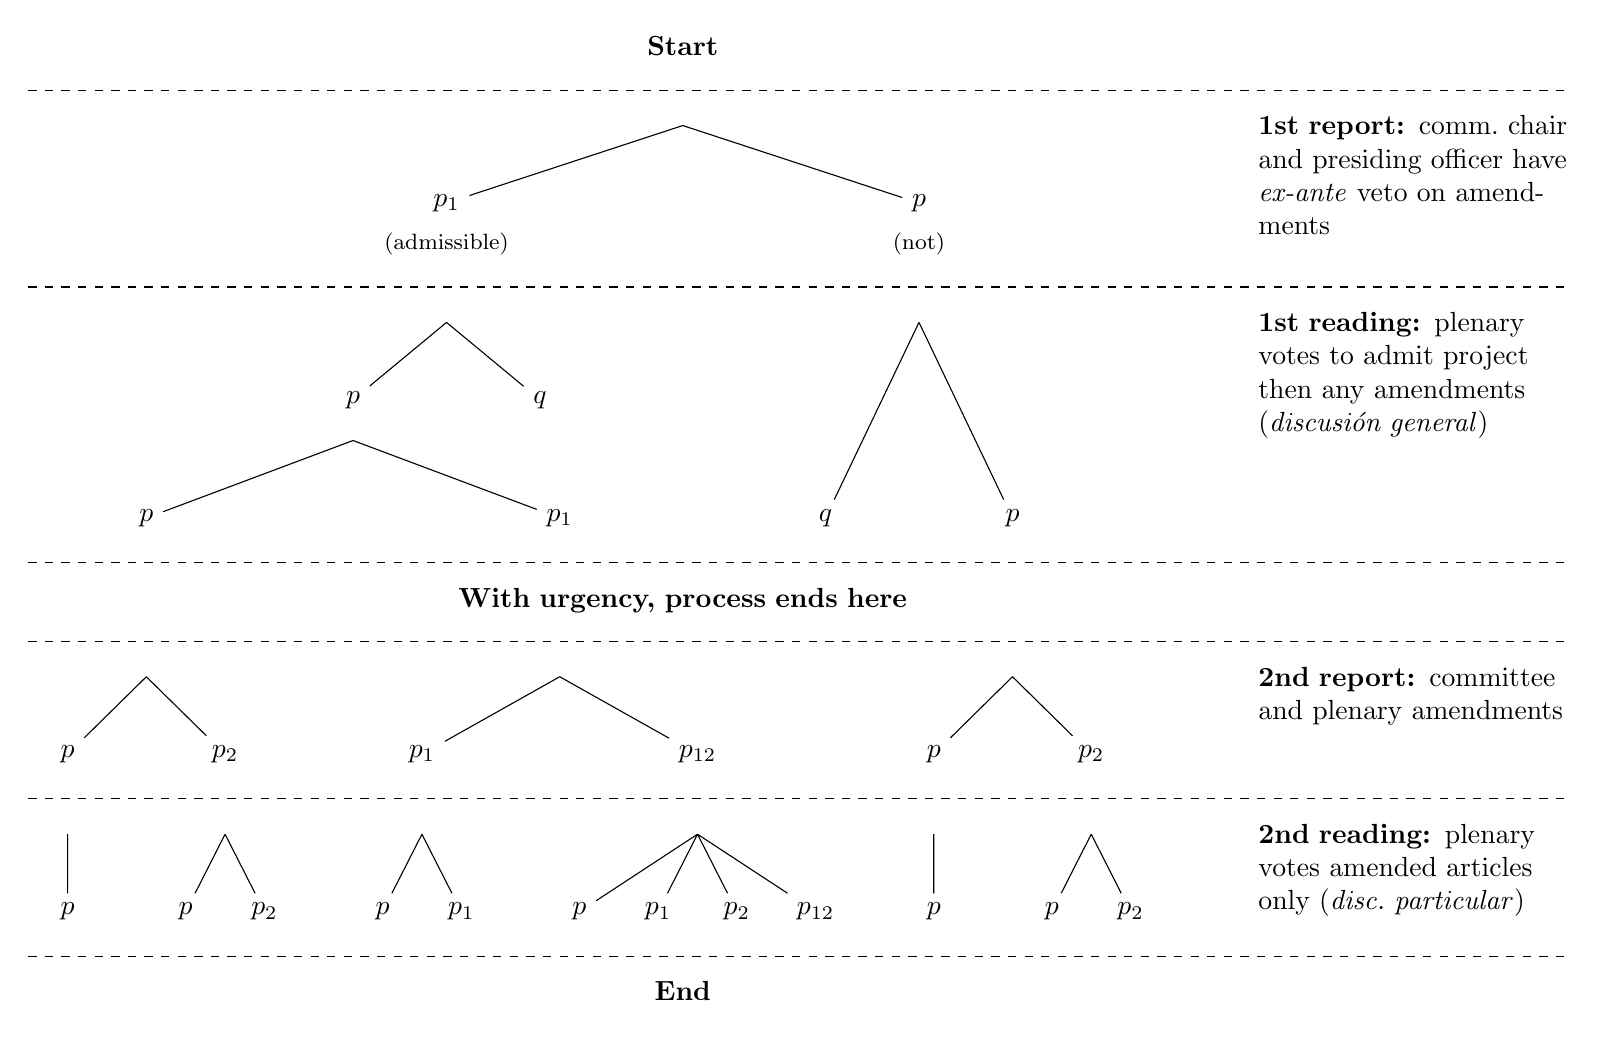
\begin{tikzpicture}
      \node[text width=10cm, text centered, anchor=north,fill=white] at (8.8125,-11) {\textbf{End}}; 
      %%%%%%%%%%%%%%%%%%%%%%%%%%%%%%%%%%%%%%%%%%%%%%%
      \draw[dashed] (0.5,-10.8) -- (20,-10.8);
      %%%%%%%%%%%%%%%%%%%%%%%%%%%%%%%%%%%%%%%%%%%%%%%
      \node[below] at (1,-10)    (o1)  {$p$}; 
      \node[below] at (2.5,-10)  (o2)  {$p$}; 
      \node[below] at (3.5,-10)  (o3)  {$p_2$}; 
      \node[below] at (5,-10)    (o4)  {$p$}; 
      \node[below] at (6,-10)    (o5)  {$p_1$}; 
      \node[below] at (7.5,-10)  (o6)  {$p$}; 
      \node[below] at (8.5,-10)  (o7)  {$p_1$}; 
      \node[below] at (9.5,-10)  (o8)  {$p_2$}; 
      \node[below] at (10.5,-10) (o9)  {$p_{12}$}; 
      \node[below] at (12,-10)   (o10) {$p$}; 
      \node[below] at (13.5,-10) (o11) {$p$}; 
      \node[below] at (14.5,-10) (o12) {$p_2$}; 
      \draw (1,-9.25) -- (o1)
            (3,-9.25) -- (o2)
            (3,-9.25) -- (o3)
            (5.5,-9.25) -- (o4)
            (5.5,-9.25) -- (o5)
            (9,-9.25) -- (o6)
            (9,-9.25) -- (o7)
            (9,-9.25) -- (o8)
            (9,-9.25) -- (o9)
            (12,-9.25) -- (o10)
            (14,-9.25) -- (o11)
            (14,-9.25) -- (o12);
      \draw[dashed] (0.5,-8.8) -- (20,-8.8);
      \node[text width=4cm, anchor=north west,fill=white] at (16,-9) {\textbf{2nd reading:} plenary votes amended articles only (\emph{disc.\ particular})}; 
      %%%%%%%%%%%%%%%%%%%%%%%%%%%%%%%%%%%%%%%%%%%%%%%
      \node[below] at (1,-8) (i21) {$p$}; 
      \node[below] at (3,-8) (i22) {$p_2$}; 
      \node[below] at (5.5,-8) (i23) {$p_1$}; 
      \node[below] at (9,-8) (i24) {$p_{12}$}; 
      \node[below] at (12,-8) (i25) {$p$}; 
      \node[below] at (14,-8) (i26) {$p_2$}; 
      \draw (2,-7.25) -- (i21)
            (2,-7.25) -- (i22)
            (7.25,-7.25) -- (i23)
            (7.25,-7.25) -- (i24)
            (13,-7.25) -- (i25)
            (13,-7.25) -- (i26);
      \draw[dashed] (0.5,-6.8) -- (20,-6.8);
      \node[text width=4cm, anchor=north west,fill=white] at (16,-7) {\textbf{2nd report:} committee and plenary amendments}; 
      % %%%%%%%%%%%%%%%%%%%%%%%%%%%%%%%%%%%%%%%%%%%%%%%
      \draw[dashed] (0.5,-5.8) -- (20,-5.8);
      \node[text width=10cm, text centered, anchor=north,fill=white] at (8.8125,-6) {\textbf{With urgency, process ends here}}; 
      %%%%%%%%%%%%%%%%%%%%%%%%%%%%%%%%%%%%%%%%%%%%%%%
      \node[below] at (2,-5) (g11) {$p$}; 
      \node[below] at (7.25,-5) (g12) {$p_1$}; 
      \node[below] at (4.625,-3.5) (g1) {$p$}; 
      \node[below] at (7,-3.5) (g2) {$q$}; 
      \node[below] at (13,-5) (g3) {$p$}; 
      \node[below] at (10.625,-5) (g4) {$q$}; 
      \draw (4.625,-4.25) -- (g11)
            (4.625,-4.25) -- (g12)
%            (13,-4.25) -- (13,-5.25)
            (5.8125,-2.75) -- (g1)
            (5.8125,-2.75) -- (g2)
            (11.8125,-2.75) -- (g3)
            (11.8125,-2.75) -- (g4);
      \draw[dashed] (0.5,-2.3) -- (20,-2.3);
      \node[text width=4cm, anchor=north west,fill=white] at (16,-2.5) {\textbf{1st reading:} plenary votes to admit project then any amendments (\emph{discusión general})}; 
      %%%%%%%%%%%%%%%%%%%%%%%%%%%%%%%%%%%%%%%%%%%%%%%
      \node[below] at (5.8125,-1) (i11) {$p_1$}; 
      \node[text width=2cm, text centered] at (5.8125,-1.75) {\footnotesize{(admissible)}}; 
      \node[below] at (11.8125,-1) (i12) {$p$}; 
      \node[text width=2cm, text centered] at (11.8125,-1.75) {\footnotesize{(not)}}; 
      \draw (8.8125,-.25) -- (i11)
            (8.8125,-.25) -- (i12);
      \draw[dashed] (0.5,.2) -- (20,.2);
      \node[text width=4cm, anchor=north west,fill=white] at (16,0) {\textbf{1st report:} comm.\ chair and presiding officer have \emph{ex-ante} veto on amendments}; 
      %%%%%%%%%%%%%%%%%%%%%%%%%%%%%%%%%%%%%%%%%%%%%%%
      \node[text width=10cm, text centered, anchor=north,fill=white] at (8.8125,1) {\textbf{Start}}; 
      %%%%%%%%%%%%%%%%%%%%%%%%%%%%%%%%%%%%%%%%%%%%%%%
    \end{tikzpicture}  \\
\end{sidewaysfigure}

We use the example to stylize the evolution of legislative proposals, from introduction to passage, in order to illustrate how urgencies affect bills. We introduce some notation. The three-article project is $p$, and $q$ the status quo (where students and teachers get \$0 from this particular subsidy). Sub-indexes distinguish versions of $p$ with articles amended: $p_1$ has article 1 amended, $p_2$ has article 2 amended, and $p_{12}$ has both articles amended. Negotiation proceeds in four steps, schematized in Figure \ref{f:agendaUrg} as per \citet[]{schwartz.2008}.\footnote{See the Cámara's standing rules (\emph{Reglamento}), especially arts.\ 118--189.} 

\begin{enumerate}
\item The question of amendment $p_1$'s admissibility into the \textbf{first report} starts it all. The choice is by the chamber's presiding officer, who has final authority to overturn the committee chair's prior decision. Admitting $p_1$ gives way to a course of play that substantially complicates down the tree. 
\item The bill's \textbf{first plenary reading} follows (rules call it \emph{discusión general}). The question here is whether the full project should be admitted for consideration or not. If not, the legislative process ends and the status quo prevails: $p$ v. $q$. Next, a vote to also admit the amendment (if any) follows. Project $p_1$ (amendment admitted) or $p$ (not) is immediately referred back to committee for a second report. 
\item If the committee concurs, then the \textbf{second report} is the outcome of the first reading. But this is an opportunity to offer new amendments, by committee members or by legislators external to the committee (with one-third plenary backing). The committee chair and the presiding officer can fail to admit these amendments too. For the sake of simplicity, the choice here is just on article 2, but there is a world of possibilities---more re-definitions, more articles, or fewer. When amended, the second report is $p_2$ or $p_{12}$, depending on the first reading being $p$ or $p_1$, respectively. 
\item The \textbf{second reading} proceeds one article at a time (\emph{discusión particular}). Importantly, this excludes the subset of articles that were not amended/added/removed in previous steps. This subset (which may include every article if none were amended) is considered adopted with no plenary vote. Rejecting article 1's amendment makes the project lose sub-index 1; likewise with article 2. So when $p_{12}$ is the second report, the plenary can accept one amendment, the other, both, or neither---as in the bottom row of Figure \ref{f:agendaUrg}. 
\end{enumerate}


We underline how the process shortens and becomes simpler when the proposal is urgent. This is a key intuition from \citet{sotoCongChile2015}: when the executive issues an urgency message, \emph{the bill takes a procedural shortcut}. As per the Lower Chamber's standing rules (arts.~188--9), urgent bills receive no second committee report, and the first and second plenary readings (\emph{discusiones general y particular} take place at once.\footnote{An additional caveat, which we do not elaborate, is that amendments rejected by the committee will only be admitted for plenary reading if signed by thirty deputies, including at least three committee chairs.} 

%%%%%%%%%%%%%%%%%%%%%%%%%%%%%%%
%% ReglamDip arts 188 y 189: %%
%%%%%%%%%%%%%%%%%%%%%%%%%%%%%%%
%% Art. 188. Cuando un proyecto sea declarado de "suma urgencia", se procederá a su discusión en la siguiente forma: No habrá segundo informe de Comisión y el proyecto deberá ser despachado por la Cámara en diez días, que se distribuirán así:
%% 1° Cinco días para el informe de Comisión.
%% 2° Tres días para el informe de la Comisión de Hacienda, si procediere.
%% 3° Dos días para la discusión y votación en la Sala.
%% La discusión se hará en general y particular a la vez. Sólo se admitirán a discusión y votación las indicaciones o disposiciones que, rechazadas por la Comisiones informantes, sean renovadas con las firmas de treinta Diputados que incluyan, a lo menos, a tres Jefes de Comités. Para tal efecto, los informes consignarán expresamente estas circunstancias.
%% Lo dispuesto en este número se debe entender sin perjuicio de lo establecido en el inciso segundo del artículo 132 (declaratoria de terminada la discusión).
%% ...
%% Art. 189. Cuando un proyecto sea declarado de "discusión inmediata", se procederá a su discusión y votación en la forma siguiente:
%% El proyecto deberá ser despachado por la Cámara en tres días, que se distribuirán así:
%% 1°.- Un día para el informe de la Comisión competente, que puede ser verbal o escrito.
%% 2°.- Un día para el informe de la Comisión de Hacienda, si procediere, que puede ser verbal o escrito.
%% 3°.- Un día para la discusión y votación del proyecto.
%% Lo dispuesto en este N° 3 deberá entenderse sin perjuicio de lo establecido en el inciso segundo del artículo 132 (renuncia de Comités a su tiempo).
%% Para los demás trámites Constitucionales tendrá la Cámara un día adicional.
%% La discusión de estos proyectos se hará en general y particular a la vez. No serán sometidos a segundo informe.
%% La Ley Orgánica no menciona nada acerca de restrictive rules. 

The urgency authority therefore equips the executive with the ability to apply a restrictive rule towards plenary consideration. The restriction consists of precluding the second round of amendments. Figure \ref{f:agendaUrg} portrays this as a break mid-way in the consideration process. With urgent consideration, when the presiding officer admits $p_1$ the plenary's choice set includes $q$, $p$, and $p_1$ only. At its most restrictive---when the presiding officer removes $p_1$ from the menu---the plenary is presented with a take-it-or-leave-it urgent proposal $p$.

This is to say, therefore, that the toolbox of formidable legislative powers of the Chilean president includes the ability to impose restrictive floor consideration rules. In Chile, the president plays the role played by the powerful Rules Committee in the U.S.\ House. In the next section we we analyze the conditions under which  Chilean presidents choose different types of rules in the legislative process. 

%% Un perfil de preferencia para ilustrar podria ser el siguiente:
%% \begin{itemize}
%% \item La mayoría está cerca de los maestros y ordena las alternativas $p_{12}>p_{2}>p_{1}>p>q$ (de mejor a peor)
%% \item El gobierno  $p>q>p_2>p_1>p_{12}$.
%% \end{itemize}

\section{Extending a model of restrictive rules to Chile}

\vp{En el pdf version 09 la figura queda antes del título de esta sección, debería quedar después porque si bien no importa dónde dentro de una sección, entre secciones me parece que confunde}
\emm{En principio, ya lo he cambiado.}

\begin{figure}
  \centering
    \caption{The president rules game. The dashed branch may be practicable, or not.}\label{F:game}
    \tikzstyle{mid}=[circle,draw]
    \begin{tikzpicture}
      % \node[rectangle,draw] (n) at (0,0) {Nature};
      %\node (n) at (0,0) {\footnotesize{(Nature): $\pi$}};
      \node[mid] at (1.5,-0.25) (c) {\emph{C}};
      \node[mid] at (4,1) (p) {\emph{P}};
      \node[mid] at (6.5,1) (f) {\emph{F}};
      \node at (4,-1.5) (ce) {$q$};
      \node at (6.5,2.25) (pe1) {$x_F$};
      \node at (6.5,-0.25) (pe2) {$q$};
      \node at (9,2.25) (fe1) {$x_C$};
      \node at (9,-0.25) (fe2) {$q$};
      % \node at (0,0.7) {\small{Strategies:}}; \node at (2,0.7)
      % {\footnotesize{---}}; \node at (4,0.7) {\footnotesize{$x^*$}};
      % \node at (6,0.7) {\footnotesize{$y^*(x)$}}; \node at (8,0.7)
      % {\footnotesize{$z^*(x)$}}; \node at (0,-1.7)
      % {\small{Outcomes:}};
      %\path[->] (n) edge (c);
      \path[-] (c) edge node [above, sloped] {\footnotesize{report}} (p)
               (p) edge node [above, sloped] {\footnotesize{ur-}} (f)
                   edge node [below, sloped] {\footnotesize{gent}} (f);
      % \path[] (n) edge node [below] {\footnotesize{$\pi$}} (c)
      \path[] (c) edge node [below, sloped] {\footnotesize{$x_C$}} (p);
      \path[-o] (c) edge node [below, sloped] {\footnotesize{not}} (ce)
                (p) edge node [above, sloped] {\footnotesize{standard}} (pe1)
%                    edge node [below, sloped] {\footnotesize{feto}} (pe2)
                (f) edge node [above, sloped] {\footnotesize{accept}} (fe1)
                    %edge node [above, sloped] {\footnotesize{ofer-}} (fe2)
                    edge node [below, sloped] {\footnotesize{reject}} (fe2);
      \path[-o, dashed] (p) edge node [below, sloped] {\footnotesize{veto}} (pe2);
    \end{tikzpicture}
\end{figure}

We stylize the Chilean urgency authority as a game of restrictive procedures inspired by \citet{dion.huber.1996}, with the president in the role of the Rules Committee. Figure \ref{F:game} portrays the game's extended form.

The main features of this game are as follows. Unless there is unanimous support to suspend the chamber's rules, every proposal requires a committee report prior to floor consideration (Organic Law, art.~21). The committee with jurisdiction over a given proposal starts the game, choosing whether or not to report the bill to the floor. No explicit discharge procedure exists in Chile. This confers gate-keeping power to committees over policy in their jurisdiction: when the committee withholds a report, the game ends with policy at the status quo $q$. Chilean committees are no different in this respect from those in the U.S.\ Congress. If a report is produced, the committee can approve the proposal in whole or in part, amend it, make additions, or reject it (Cámara standing rule 287.8). We interpret this as (positive) agenda power to locate the proposal in policy space: $x_C \in [0,1]$. The president moves next. 

The president's choice set has three alternatives: let the bill proceed under standard floor consideration; declare it urgent; or issue a veto. Standard consideration ends the game with policy at $x_F$. By navigating the plenary session with an open rule, amendments reshape the bill to the floor's liking. As in \citet{shepsle.1979}, we take $x_F$ to be the floor median's ideal point, corresponding to a game of full plenary influence. The next alternative, urgency, invokes the restrictive consideration rule and presents the floor with a take-it-or-leave-it offer. Unable to amend the proposal, the floor, which moves after the bill was marked urgent, must choose between the reported bill $x_C$ or the status quo, as in \citep{romer.rosenthal.1978}. The final presidential alternative, the veto, may end the game at the status quo---the formal equivalent of the rule denial in Dion and Huber's procedural stage.

\vp{But this [open rule] returns the bill to the committee, no?}
\emm{Presumably... but model totally ignores this. Simplistic? Justifiable? May need some elaboration.}
\ges{I think is good as is, although I'm still not clear in the type of amendments that legislators can introduce in the consideracion en general. Con el ejemplo pareciera que es cualquier tipo de amendment? Me imagino que no, pero no me queda claro como es el tema en la votacion en general.  Si, se vota toda la ley, y los legisladores pueden ofrecer una ley alternativa? si ? no?}

%This ``veto'' is a stylization of events taking place much later in the actual legislative process, after the approved bill lands on the president's desk. For the executive veto to exert an influence so much earlier in the process, players must entertain the expectation that it will be sustained, effectively reinstating the status quo. This tree branch will therefore not be practicable when there is no way to fully discard the possibility of a veto override. The dashed line in Figure \ref{F:game} indicates that the branch may or may not be part of the president's choice set. We analyze versions of the game with (``veto will be sustained'') and without (``veto will be overridden'') the dashed line. 

This ``veto'' is a stylization of events taking place much later in the actual legislative process, after the approved bill lands on the president's desk. The specific features of the presidential veto in Chile call for a caveat. The veto takes on different forms in Chile, such that the president may choose to veto the bill completely (total veto), or do a number of things to alter the bill partially.\footnote{The president may delete parts of the bill, add parts to the bill, and also change parts of the bill (which combines deleting and adding).} For the executive veto to exert an influence so much earlier in the game, players must entertain the expectation that it will be sustained, effectively reinstating the status quo. In Chile, between 1990 and 2014 only one total veto took place, and it was not overridden---so while the likelihood of total vetoes and of overrides are both low, neither can be completely discarded. This branch will therefore not be practicable when there is no way to fully discard the possibility of a veto override. The dashed line in Figure \ref{F:game} indicates that the branch may or may not be part of the president's choice set. We analyze versions of the game with and without the dashed line. 

\begin{figure}
  \centering
  \caption{Illustration of the equilibrium proposal when the veto is practicable (v) or not (\~v)}\label{F:example}
  \begin{tikzpicture}[scale=.9]
    \draw (0,0) -- (13,0);% node[right] {$q \in X$};
    \draw[dashed] (2,0) -- (3,0.5) -- (4,0);
    \draw[dashed] (2,0) -- (7.25,2.625) -- (12.5,0);
    \draw (0,0.1) -- (0,-0.1) node[below=-0.1] {$0$}
    (1,0.1) -- (1,-0.1) node[below=-0.1] {\textcolor{gray}{$P_C$}}
    (2,0.1) -- (2,-0.1) node[below=-0.1] {$q$}
    (3,0.1) -- (3,-0.1) node[below=-0.1] {$P$}
    (4,0.1) -- (4,-0.1) node[below=-0.1] {$P_q$}
    (5,0.1) -- (5,-0.1) node[below=-0.1] {$C$}
    (7.25,0.1) -- (7.25,-0.1) node[below=-0.1] {$F$}
    (9.5,0.1) -- (9.5,-0.1) node[below=-0.1] {\textcolor{gray}{$F_C$}}
    (12.5,0.1) -- (12.5,-0.1) node[below=-0.1] {$F_q$}
    (13,0.1) -- (13,-0.1) node[below=-0.1] {$1$};
    \draw[->] (4,.5) node[above=-0.1] {v} -- (4,.15);
    \draw[->] (5,.5) node[above=-0.1] {\~v} -- (5,.15);
  \end{tikzpicture}
\end{figure}

Model analysis is analogous to \citet{dion.huber.1996}. The game has a unique, sub-game perfect equilibrium that we do not derive formally here.\footnote{Equilibrium is akin to \citet{magar.nd,romer.rosenthal.1978,cox.mccubbins.2005,gerber.1996}. There seem to be minor inconsistencies between the equilibrium that Dion and Huber portray in their Figure 1 and ours here.} We elaborate the bargaining logic with the example in Figure \ref{F:example}. $P$, $C$, and $F$ represent the ideal points of the president, the committee, and the floor, respectively, while $q$ is the status quo. $F_q$ is the reflection of $q$ on $F$ (more precisely, the symmetric reflection of $q$ in space using $F$ as axis). Other relevant reflections are noted likewise; some appear in gray and will be relevant later. As the model assumes standard Euclidian preferences and reflections point to equidistance in the opposite side of an ideal point, preference is easily gauged: the floor finds policy under the larger dashed pyramid ($x_C \in [q,F_q]$) preferable to the status quo; likewise, the president prefers policy under the smaller pyramid ($x_C \in [q,P_q]$) to the status quo. 

Deriving optimal proposal and consideration regime is trivial. Proceeding backwards in the game tree, the floor will accept proposals under the larger pyramid, reject the rest. So everyone anticipates that urgent consideration of proposal $x_C \in [q,F_q]$ beats the status quo. Also, because in the example $F$ is outside the smaller pyramid, all anticipate that the president discards standard consideration ($x_F=F$ would be the outcome). Therefore, when (1) $x_C$ is inside the smaller pyramid, or (2) the veto branch is impracticable, the president chooses urgent consideration; otherwise s/he vetoes. Proposal $x_C=P_q$ meets conditions to avoid a practicable veto while maximizing committee welfare (the arrow with a v above points to it in the Figure). With impracticable veto the committee can afford to send $x_C=C$ (the arrow with \~v on top).

\begin{figure}
  \centering
    \caption{Comparative statics with variable status quo}\label{F:predictions}
    \scalebox{.85}{
      \begin{tabular}{l} 
        \textbf{Profile I:} $P < C < F$ \\ 
        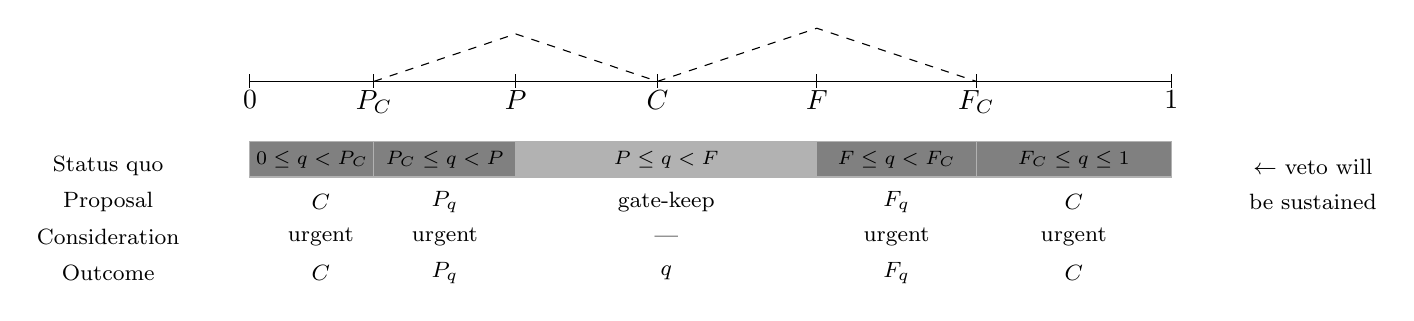
\begin{tikzpicture}[scale=.9]
          \draw (0,0) -- (13,0);% node[right] {$q \in X$};
          \draw[dashed] (1.75,0) -- (3.75,0.67) -- (5.75,0);
          \draw[dashed] (5.75,0) -- (8,.75) -- (10.25,0);
          \draw (0,0.1) -- (0,-0.1) node[below=-0.1] {$0$}
          (1.75,0.1) -- (1.75,-0.1) node[below=-0.1] {$P_C$}
          (3.75,0.1) -- (3.75,-0.1) node[below=-0.1] {$P$}
          (5.75,0.1) -- (5.75,-0.1) node[below=-0.1] {$C$}
          (8,0.1) -- (8,-0.1) node[below=-0.1] {$F$}
          (10.25,0.1) -- (10.25,-0.1) node[below=-0.1] {$F_C$}
          (13,0.1) -- (13,-0.1) node[below=-0.1] {$1$};
          \node at (-2,-2.7) {\footnotesize{Outcome}};
          \node at (-2,-2.2) {\footnotesize{Consideration}};
          \node at (-2,-1.7)  {\footnotesize{Proposal}};
          \node at (-2,-1.2)  {\footnotesize{Status quo}};
          \node at (15,-1.2)  {\footnotesize{$\leftarrow$ veto will}};
          \node at (15,-1.7)  {\footnotesize{be sustained}};
          \node at (1,-2.7)   {\footnotesize{$C$}};        % Outcome      
          \node at (1,-2.2) {\footnotesize{urgent}};       % Consideration
          \node at (1,-1.7)   {\footnotesize{$C$}};        % Proposal     
          \node at (2.75,-2.7)   {\footnotesize{$P_q$}};        % Outcome      
          \node at (2.75,-2.2) {\footnotesize{urgent}};       % Consideration
          \node at (2.75,-1.7)   {\footnotesize{$P_q$}};        % Proposal     
          \node at (5.875,-2.7)   {\footnotesize{$q$}};       % Outcome      
          \node at (5.875,-2.2) {\footnotesize{---}};           % Consideration
          \node at (5.875,-1.7)   {\footnotesize{gate-keep}};    % Proposal     
          \node at (9.125,-2.7)   {\footnotesize{$F_q$}};       % Outcome      
          \node at (9.125,-2.2) {\footnotesize{urgent}};        % Consideration
          \node at (9.125,-1.7)   {\footnotesize{$F_q$}};       % Proposal     
          \node at (11.625,-2.7)   {\footnotesize{$C$}};          % Outcome      
          \node at (11.625,-2.2) {\footnotesize{urgent}};         % Consideration
          \node at (11.625,-1.7)   {\footnotesize{$C$}};          % Proposal     
          \filldraw[fill=black!50,draw=black!30]   (0,-1.35) rectangle node {\scriptsize{$0 \leq q < P_C$}} (1.75,-0.85);
          \filldraw[fill=black!50,draw=black!30]   (1.75,-1.35) rectangle node {\scriptsize{$P_C \leq q < P$}} (3.75,-0.85);
          \filldraw[fill=black!30,draw=black!30]  (3.75,-1.35) rectangle node {\scriptsize{$P \leq q < F$}} (8,-0.85);
          \filldraw[fill=black!50,draw=black!30]  (8,-1.35) rectangle node {\scriptsize{$F \leq q < F_C$}} (10.25,-0.85);
          \filldraw[fill=black!50,draw=black!30]  (10.25,-1.35) rectangle node {\scriptsize{$F_C \leq q \leq 1$}} (13,-0.85);
        \end{tikzpicture} \\ \\

        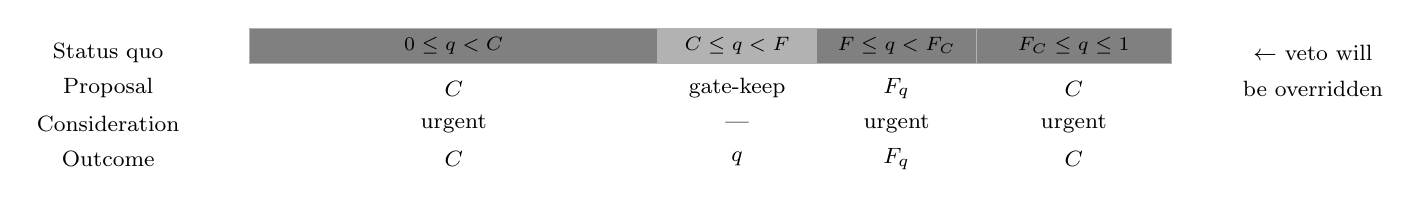
\begin{tikzpicture}[scale=.9]
          %% \draw (0,0) -- (13,0);% node[right] {$q \in X$};
          %% \draw[dashed] (1.75,0) -- (3.75,0.67) -- (5.75,0);
          %% \draw[dashed] (5.75,0) -- (8,.75) -- (10.25,0);
          %% \draw (0,0.1) -- (0,-0.1) node[below=-0.1] {$0$}
          %% (1.75,0.1) -- (1.75,-0.1) node[below=-0.1] {$P_C$}
          %% (3.75,0.1) -- (3.75,-0.1) node[below=-0.1] {$P$}
          %% (5.75,0.1) -- (5.75,-0.1) node[below=-0.1] {$C$}
          %% (8,0.1) -- (8,-0.1) node[below=-0.1] {$F$}
          %% (10.25,0.1) -- (10.25,-0.1) node[below=-0.1] {$F_C$}
          %% (13,0.1) -- (13,-0.1) node[below=-0.1] {$1$};
          \node at (-2,-2.7) {\footnotesize{Outcome}};
          \node at (-2,-2.2) {\footnotesize{Consideration}};
          \node at (-2,-1.7)  {\footnotesize{Proposal}};
          \node at (-2,-1.2)  {\footnotesize{Status quo}};
          \node at (15,-1.2)  {\footnotesize{$\leftarrow$ veto will}};
          \node at (15,-1.7)  {\footnotesize{be overridden}};
          \node at (2.875,-2.7)   {\footnotesize{$C$}};          % Outcome      
          \node at (2.875,-2.2) {\footnotesize{urgent}};         % Consideration
          \node at (2.875,-1.7)   {\footnotesize{$C$}};          % Proposal     
          \node at (6.875,-2.7)   {\footnotesize{$q$}};        % Outcome      
          \node at (6.875,-2.2) {\footnotesize{---}};            % Consideration
          \node at (6.875,-1.7)   {\footnotesize{gate-keep}};     % Proposal     
          \node at (9.125,-2.7)   {\footnotesize{$F_q$}};        % Outcome      
          \node at (9.125,-2.2) {\footnotesize{urgent}};         % Consideration
          \node at (9.125,-1.7)   {\footnotesize{$F_q$}};        % Proposal     
          \node at (11.625,-2.7)   {\footnotesize{$C$}};          % Outcome      
          \node at (11.625,-2.2) {\footnotesize{urgent}};         % Consideration
          \node at (11.625,-1.7)   {\footnotesize{$C$}};          % Proposal     
          \filldraw[fill=black!50,draw=black!30]   (0,-1.35) rectangle node {\scriptsize{$0 \leq q < C$}} (5.75,-0.85);
          \filldraw[fill=black!30,draw=black!30]  (5.75,-1.35) rectangle node {\scriptsize{$C \leq q < F$}} (8,-0.85);
          \filldraw[fill=black!50,draw=black!30]  (8,-1.35) rectangle node {\scriptsize{$F \leq q < F_C$}} (10.25,-0.85);
          \filldraw[fill=black!50,draw=black!30]  (10.25,-1.35) rectangle node {\scriptsize{$F_C \leq q \leq 1$}} (13,-0.85);
        \end{tikzpicture} \\ \\

        \textbf{Profile II:} $C \leq P \leq F$ \\ 
        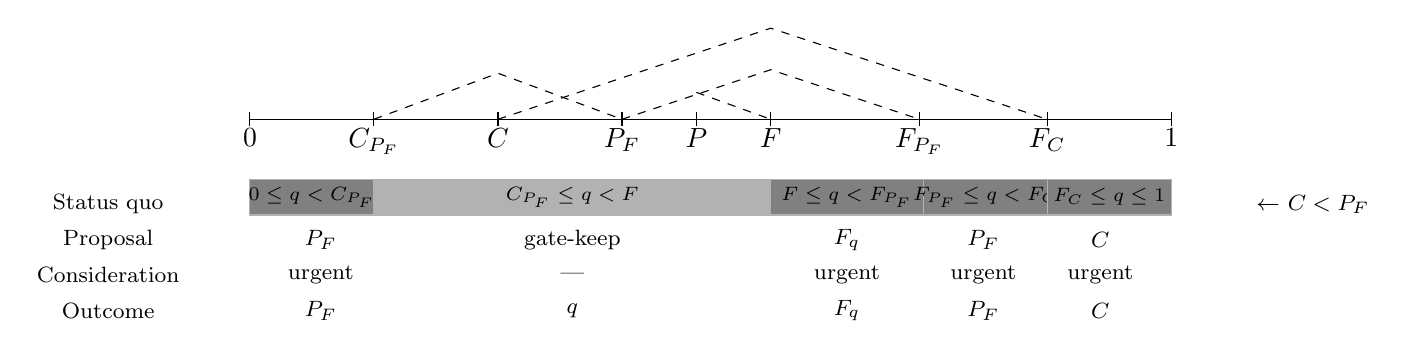
\begin{tikzpicture}[scale=.9]
          \draw (0,0) -- (13,0);% node[right] {$q \in X$};
          \draw[dashed] (1.75,0) -- (3.5,0.65) -- (5.25,0);
          \draw[dashed] (3.5,0) -- (7.35,1.285) -- (11.25,0);
          \draw[dashed] (5.25,0) -- (7.35,.7) -- (9.45,0);
          \draw[dashed] (6.3,0.38) -- (7.35,0);
          \draw (0,0.1) -- (0,-0.1) node[below=-0.1] {$0$}
          (1.75,0.1) -- (1.75,-0.1) node[below=-0.1] {$C_{P_F}$}
          (3.5,0.1) -- (3.5,-0.1) node[below=-0.1] {$C$}
          (5.25,0.1) -- (5.25,-0.1) node[below=-0.1] {$P_F$}
          (6.3,0.1) -- (6.3,-0.1) node[below=-0.1] {$P$}
          (7.35,0.1) -- (7.35,-0.1) node[below=-0.1] {$F$}
          (9.45,0.1) -- (9.45,-0.1) node[below=-0.1] {$F_{P_F}$}
          (11.25,0.1) -- (11.25,-0.1) node[below=-0.1] {$F_C$}
          (13,0.1) -- (13,-0.1) node[below=-0.1] {$1$};
          \node at (-2,-2.7) {\footnotesize{Outcome}};
          \node at (-2,-2.2) {\footnotesize{Consideration}};
          \node at (-2,-1.7)  {\footnotesize{Proposal}};
          \node at (-2,-1.2)  {\footnotesize{Status quo}};
          \node at (15,-1.2)  {\footnotesize{$\leftarrow$ $C<P_F$}};
          \node at (1,-2.7)   {\footnotesize{$P_F$}};           % Outcome      
          \node at (1,-2.2) {\footnotesize{urgent}};            % Consideration
          \node at (1,-1.7)   {\footnotesize{$P_F$}};           % Proposal     
          \node at (4.55,-2.7)   {\footnotesize{$q$}};           % Outcome      
          \node at (4.55,-2.2) {\footnotesize{---}};               % Consideration
          \node at (4.55,-1.7)   {\footnotesize{gate-keep}};        % Proposal     
          \node at (8.425,-2.7)   {\footnotesize{$F_q$}};           % Outcome      
          \node at (8.425,-2.2) {\footnotesize{urgent}};            % Consideration
          \node at (8.425,-1.7)   {\footnotesize{$F_q$}};           % Proposal     
          \node at (10.35,-2.7)   {\footnotesize{$P_F$}};           % Outcome      
          \node at (10.35,-2.2) {\footnotesize{urgent}};            % Consideration
          \node at (10.35,-1.7)   {\footnotesize{$P_F$}};           % Proposal     
          \node at (12,-2.7)   {\footnotesize{$C$}};             % Outcome      
          \node at (12,-2.2) {\footnotesize{urgent}};            % Consideration
          \node at (12,-1.7)   {\footnotesize{$C$}};             % Proposal     
          \filldraw[fill=black!50,draw=black!30]   (0,-1.35) rectangle node {\scriptsize{$0 \leq q < C_{P_F}$}} (1.75,-0.85);
          \filldraw[fill=black!30,draw=black!30]  (1.75,-1.35) rectangle node {\scriptsize{$C_{P_F} \leq q < F$}} (7.35,-0.85);
          \filldraw[fill=black!50,draw=black!30]  (7.35,-1.35) rectangle node {\scriptsize{$F \leq q < F_{P_F}$}} (9.5,-0.85);
          \filldraw[fill=black!50,draw=black!30]  (9.5,-1.35) rectangle node {\scriptsize{$F_{P_F} \leq q < F_C$}} (11.25,-0.85);
          \filldraw[fill=black!50,draw=black!30]  (11.25,-1.35) rectangle node {\scriptsize{$F_C \leq q \leq 1$}} (13,-0.85);
        \end{tikzpicture} \\ \\

        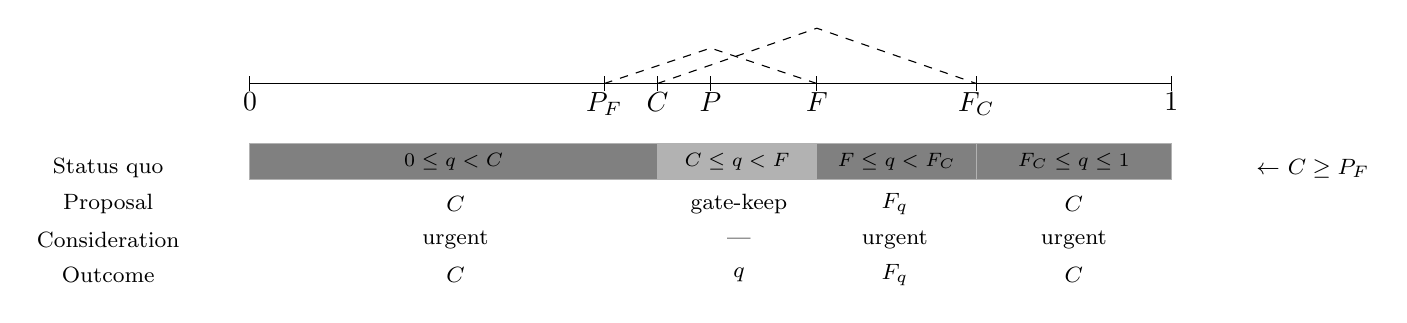
\begin{tikzpicture}[scale=.9]
          \draw (0,0) -- (13,0);% node[right] {$q \in X$};
          \draw[dashed] (5,0) -- (6.5,0.5) -- (8,0);
          \draw[dashed] (5.75,0) -- (8,.78) -- (10.25,0);
          \draw (0,0.1) -- (0,-0.1) node[below=-0.1] {$0$}
          (5,0.1) -- (5,-0.1) node[below=-0.1] {$P_F$}
          (5.75,0.1) -- (5.75,-0.1) node[below=-0.1] {$C$}
          (6.5,0.1) -- (6.5,-0.1) node[below=-0.1] {$P$}
          (8,0.1) -- (8,-0.1) node[below=-0.1] {$F$}
          (10.25,0.1) -- (10.25,-0.1) node[below=-0.1] {$F_C$}
          (13,0.1) -- (13,-0.1) node[below=-0.1] {$1$};
          \node at (-2,-2.7) {\footnotesize{Outcome}};
          \node at (-2,-2.2) {\footnotesize{Consideration}};
          \node at (-2,-1.7)  {\footnotesize{Proposal}};
          \node at (-2,-1.2)  {\footnotesize{Status quo}};
          \node at (15,-1.2)  {\footnotesize{$\leftarrow$ $C \geq P_F$}};
          \node at (2.9,-2.7)   {\footnotesize{$C$}};        % Outcome      
          \node at (2.9,-2.2) {\footnotesize{urgent}};       % Consideration
          \node at (2.9,-1.7)   {\footnotesize{$C$}};        % Proposal     
          \node at (6.9,-2.7)   {\footnotesize{$q$}};      % Outcome      
          \node at (6.9,-2.2) {\footnotesize{---}};          % Consideration
          \node at (6.9,-1.7)   {\footnotesize{gate-keep}};   % Proposal     
          \node at (9.1,-2.7)   {\footnotesize{$F_q$}};      % Outcome      
          \node at (9.1,-2.2) {\footnotesize{urgent}};       % Consideration
          \node at (9.1,-1.7)   {\footnotesize{$F_q$}};      % Proposal     
          \node at (11.625,-2.7)   {\footnotesize{$C$}};         % Outcome      
          \node at (11.626,-2.2) {\footnotesize{urgent}};        % Consideration
          \node at (11.625,-1.7)   {\footnotesize{$C$}};         % Proposal     
          \filldraw[fill=black!50,draw=black!30]   (0,-1.35) rectangle node {\scriptsize{$0 \leq q < C$}} (5.75,-0.85);
          \filldraw[fill=black!30,draw=black!30]  (5.75,-1.35) rectangle node {\scriptsize{$C \leq q < F$}} (8,-0.85);
          \filldraw[fill=black!50,draw=black!30]  (8,-1.35) rectangle node {\scriptsize{$F \leq q < F_C$}} (10.25,-0.85);
          \filldraw[fill=black!50,draw=black!30]  (10.25,-1.35) rectangle node {\scriptsize{$F_C \leq q \leq 1$}} (13,-0.85);
        \end{tikzpicture} \\ \\

        \textbf{Profile III:} $C <  F <  P$ \\ 
        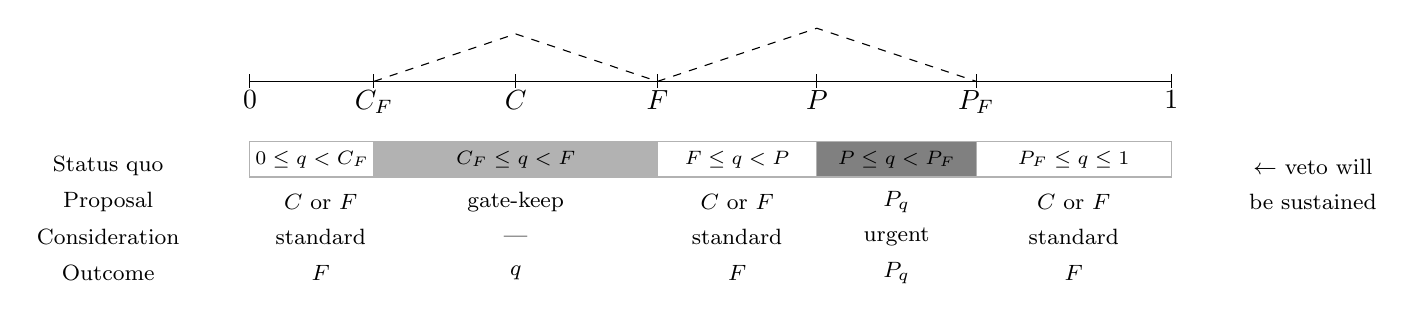
\begin{tikzpicture}[scale=.9]
          \draw (0,0) -- (13,0);% node[right] {$q \in X$};
          \draw[dashed] (1.75,0) -- (3.75,0.67) -- (5.75,0);
          \draw[dashed] (5.75,0) -- (8,.75) -- (10.25,0);
          \draw (0,0.1) -- (0,-0.1) node[below=-0.1] {$0$}
          (1.75,0.1) -- (1.75,-0.1) node[below=-0.1] {$C_F$}
          (3.75,0.1) -- (3.75,-0.1) node[below=-0.1] {$C$}
          (5.75,0.1) -- (5.75,-0.1) node[below=-0.1] {$F$}
          (8,0.1) -- (8,-0.1) node[below=-0.1] {$P$}
          (10.25,0.1) -- (10.25,-0.1) node[below=-0.1] {$P_F$}
          (13,0.1) -- (13,-0.1) node[below=-0.1] {$1$};
          \node at (-2,-2.7) {\footnotesize{Outcome}};
          \node at (-2,-2.2) {\footnotesize{Consideration}};
          \node at (-2,-1.7)  {\footnotesize{Proposal}};
          \node at (-2,-1.2)  {\footnotesize{Status quo}};
          \node at (15,-1.2)  {\footnotesize{$\leftarrow$ veto will}};
          \node at (15,-1.7)  {\footnotesize{be sustained}};
          \node at (1,-2.7)   {\footnotesize{$F$}};              % Outcome      
          \node at (1,-2.2) {\footnotesize{standard}};           % Consideration
          \node at (1,-1.7)   {\footnotesize{$C$ or $F$}};       % Proposal     
          \node at (3.75,-2.7)   {\footnotesize{$q$}};         % Outcome      
          \node at (3.75,-2.2) {\footnotesize{---}};             % Consideration
          \node at (3.75,-1.7)   {\footnotesize{gate-keep}};      % Proposal     
          \node at (6.875,-2.7)   {\footnotesize{$F$}};          % Outcome      
          \node at (6.875,-2.2) {\footnotesize{standard}};       % Consideration
          \node at (6.875,-1.7)   {\footnotesize{$C$ or $F$}};   % Proposal     
          \node at (9.125,-2.7)   {\footnotesize{$P_q$}};        % Outcome      
          \node at (9.125,-2.2) {\footnotesize{urgent}};         % Consideration
          \node at (9.125,-1.7)   {\footnotesize{$P_q$}};        % Proposal     
          \node at (11.625,-2.7)   {\footnotesize{$F$}};         % Outcome      
          \node at (11.625,-2.2) {\footnotesize{standard}};        % Consideration
          \node at (11.625,-1.7)   {\footnotesize{$C$ or $F$}};     % Proposal     
          \filldraw[fill=black!0,draw=black!30]   (0,-1.35) rectangle node {\scriptsize{$0 \leq q < C_F$}} (1.75,-0.85);
          \filldraw[fill=black!30,draw=black!30]  (1.75,-1.35) rectangle node {\scriptsize{$C_F \leq q < F$}} (5.75,-0.85);
          \filldraw[fill=black!0,draw=black!30]  (5.75,-1.35) rectangle node {\scriptsize{$F \leq q < P$}} (8,-0.85);
          \filldraw[fill=black!50,draw=black!30]  (8,-1.35) rectangle node {\scriptsize{$P \leq q < P_F$}} (10.25,-0.85);
          \filldraw[fill=black!0,draw=black!30]  (10.25,-1.35) rectangle node {\scriptsize{$P_F \leq q \leq 1$}} (13,-0.85);
        \end{tikzpicture} \\ \\

        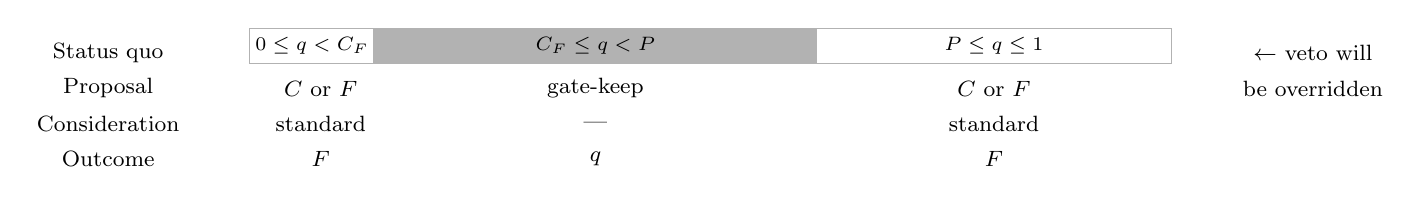
\begin{tikzpicture}[scale=.9]
          %% \draw (0,0) -- (13,0);% node[right] {$q \in X$};
          %% \draw[dashed] (1.75,0) -- (3.75,0.67) -- (5.75,0);
          %% \draw[dashed] (5.75,0) -- (8,.75) -- (10.25,0);
          %% \draw (0,0.1) -- (0,-0.1) node[below=-0.1] {$0$}
          %% (1.75,0.1) -- (1.75,-0.1) node[below=-0.1] {$C_F$}
          %% (3.75,0.1) -- (3.75,-0.1) node[below=-0.1] {$C$}
          %% (5.75,0.1) -- (5.75,-0.1) node[below=-0.1] {$F$}
          %% (8,0.1) -- (8,-0.1) node[below=-0.1] {$P$}
          %% (10.25,0.1) -- (10.25,-0.1) node[below=-0.1] {$P_F$}
          %% (13,0.1) -- (13,-0.1) node[below=-0.1] {$1$};
          \node at (-2,-2.7) {\footnotesize{Outcome}};
          \node at (-2,-2.2) {\footnotesize{Consideration}};
          \node at (-2,-1.7)  {\footnotesize{Proposal}};
          \node at (-2,-1.2)  {\footnotesize{Status quo}};
          \node at (15,-1.2)  {\footnotesize{$\leftarrow$ veto will}};
          \node at (15,-1.7)  {\footnotesize{be overridden}};
          \node at (1,-2.7)   {\footnotesize{$F$}};              % Outcome      
          \node at (1,-2.2) {\footnotesize{standard}};           % Consideration
          \node at (1,-1.7)   {\footnotesize{$C$ or $F$}};              % Proposal     
          \node at (4.875,-2.7)   {\footnotesize{$q$}};         % Outcome      
          \node at (4.875,-2.2) {\footnotesize{---}};             % Consideration
          \node at (4.875,-1.7)   {\footnotesize{gate-keep}};      % Proposal     
          \node at (10.5,-2.7)   {\footnotesize{$F$}};          % Outcome      
          \node at (10.5,-2.2) {\footnotesize{standard}};       % Consideration
          \node at (10.5,-1.7)   {\footnotesize{$C$ or $F$}};   % Proposal     
          \filldraw[fill=black!0,draw=black!30]   (0,-1.35) rectangle node {\scriptsize{$0 \leq q < C_F$}} (1.75,-0.85);
          \filldraw[fill=black!30,draw=black!30]  (1.75,-1.35) rectangle node {\scriptsize{$C_F \leq q < P$}} (8,-0.85);
          \filldraw[fill=black!0,draw=black!30]  (8,-1.35) rectangle node {\scriptsize{$P \leq q \leq 1$}} (13,-0.85);
        \end{tikzpicture} \\ \\

      \end{tabular}
    }
\end{figure}

We now derive empirical implications from our theoretical model by generalizing the bargaining logic across preference profiles in Figure \ref{F:predictions} and do comparative statics analysis. A preference profile is an ordering of players' ideal points in space. Only three of six mutually-exclusive and exhaustive profiles are portrayed: $P<C<F$, $C \leq P \leq F$, and $C<F<P$ (the other three are mirror-images). In each, the status quo is treated as a continuous variable $q \in [0,1]$. We aim to trace how changes in $q$ affect equilibrium elements---the proposal, the consideration regime, and the outcome---in each profile.

The example discussed falls under profile I (the status quo falls where $P_C \leq q < P$). The top panel in profile I represents situations where the veto branch of the game tree is practicable (the expectation is a sustained veto, as indicated at the right end), the lower panel situations where it is impracticable (a veto override is expected). The equilibrium proposal and consideration regime discussed above, and the equilibrium outcome are listed accordingly. The discrete zones into which the policy space subdivides (the dark-gray, light-gray, and white rectangles) isolate status quos with unchanging equilibrium elements. One or more equilibrium elements mutate for status quos falling in the adjacent zone(s).

We pay attention to consideration regimes: in equilibrium, status quos in dark-gray zones trigger urgent consideration, and those in white zones trigger standard consideration. Status quos in light-gray zones lack a consideration regime because they push the committee to defend the status quo by withholding the bill's report (gate-keeping). Aided by auxiliary assumptions, empirical implications follow from comparative statics. We discuss three; many more hypotheses could be derived.

To start, note how the dark-gray zones predominate in Figure \ref{F:predictions} over the light-gray and white. Urgent status corresponds to dark-gray, and the first theoretical prediction follows.

\begin{description}
  \item [Hypothesis 1] Other things constant, urgent bill consideration is likelier than standard bill consideration. 
\end{description}
    
\noindent The supporting auxiliary assumptions are two: (1) a stochastic status quo with uniform probability density in $[0,1]$ is assumed; and that (2) preference profiles I, II, and III in the Figure are equiprobable. Auxiliary assumption can be relaxed, within limits, without invalidating this prediction. 

Also plain in the Figure is that white areas, corresponding to standard bill consideration, occur under profile III only. The president's and the committee's ideal points stand on either side of the floor median in profile III, but on the same side in I and II. If these conditions are readily visible in theory, preference unobservability is an obstacle towards a test. Auxiliary assumptions therefore need discussion before putting a hypothesis forth: (1) chairs are dictators in their committee's jurisdiction; and (2) party determines ideal points. The first auxiliary assumption sets procedure in such way that the committee can be construed as a unitary actor. The second associates player preferences to something observable: parties. The next theoretical prediction follows. 

\begin{description}
  \item [Hypothesis 2.a] Other things constant, standard bill consideration does not occur when the chair of the reporting committee belongs to the president's party. 
\end{description}

\noindent Given well-documented presidential coalition discipline in Chile \citep{aleman.saiegh.coalUnityChile.2007,carey.2002}, we replace `party' by `coalition' as measure of preferences for an alternative. 

\begin{description}
  \item [Hypothesis 2.b] Other things constant, standard bill consideration does not occur when the chair of the reporting committee belongs to the president's coalition. 
\end{description}

For the next implication, see what happens when the distance separating $C$ and $P$ remains fixed while the distance between $C$ and $F$ shrinks. The size of the gate-keeping light-gray zone either remains unchanged (in Figure \ref{F:predictions}'s top panel) or also shrinks (in the remainder). The latter is quite plain in the second to next-to-last panels, where $F$ sets the upper limit of the light-gray zone. In the bottom panel, $F$ is within the light-gray zone, but its symmetric projection $C_F$ is the lower limit: sliding $F$ towards $C$ achieves the same, sliding $C_F$ towards $C$ does too. This projection game in the top panel involves both $P_F$ and $C_{p_F}$, sliding symmetrically in opposite directions to leave the size of the light-gray area unchanged. Reliance on similar auxiliary assumptions generates the next theoretical prediction.

\begin{description}
  \item [Hypothesis 3] Other things constant, the likelihood of gate-keeping is never larger when the bill's reporting committee chair belongs to to the president's coalition than to the opposition. 
\end{description}

\emm{Compact transition here.}

\section{Urgency predictors}

A systematic analysis of data in Table \ref{T:billDescriptives} is revealing. The units are individual proposals: the dependent variable \emph{Urgent bill} equals 1 for proposals that became urgent at any point of the legislative process, 0 otherwise. It excludes `one month' deadlines, which do not trigger restrictive rules (including them does not change the reported results in a fundamental way, see the appendix). Multivariate analysis controls for president--reporting committee preference coincidence, for bill features, for timing, and for the strategic environment. Formal variable definitions and descriptive statistics appear in the appendix.

The preference group includes two regressors. The first has two alternative specifications: \emph{Co-partisan comm.\ chair}, equal 1 if the bill was referred to a standing committee presided by a member of the president's party, 0 otherwise; or \emph{Coalition comm.\ chair}, equal 1 for bills referred to committees chaired by members of any party in the presidential coalition, 0 otherwise. This is our key explanatory variable, measuring spatial proximity between the chief executive and the reporting committee. Other things constant, we expect the variable to associate positively with the dependent variable under both specifications. Table \ref{T:chairsSeats} shows in part A how the number of standing committee chairs from the president's party oscillated sharply in the period, from a high of 53 percent in the 1998--2002 Legislatura, to a low of 17 percent in 2006--10. And the opposition was \todo{Check why dcoal dummy won't drop in model 3?} absent among standing committee chairs in 2006--10 only, controlling up to 24 and 27 percent in 2002--06 and 2010--14, respectively.\footnote{\emph{Largesse} towards opposition parties was probably aimed at beefing up the president's legislative support. The Table's parts B and C report variance in the size and status of the president's coalition in Congress. Given electoral list voting unity since the return to democracy \citep{carey.2002,aleman.saiegh.coalUnityChile.2007}, the seats they control are a good indicator of the executive's legislative support. The coalition remained in control of the Cámara throughout the period, but controlled Senate majorities between 2006 and 2010 only (coinciding with the first Bachelet administration). By requiring 67, 60, and 57 percent votes of each chamber, respectively, constitutional reform, constitution-interpreting legislation, and organic laws therefore always required support across the aisle.} 

\begin{table}
\centering
\caption{The president's status in Congress and its committees. Percent chairs/seats by party. The president's coalition in 1998--2010 was Concertación; it was Alianza afterwards. Regional includes major-party splinters (from Christian Democrats and UDI). President's status in the Senate slightly and briefly oscillated above and below majority due to vacant seats. Source: prepared with information from \protect\url{www.camara.cl}.}\label{T:chairsSeats}
\begin{tabular}{lrrrr}
                      & 1998--2002 & 2002--06 & 2006--10 & 2010--14 \\ \hline
\mc{5}{c}{\textbf{~~Part A. Committee chairs, Cámara}} \\
President's party     &  \emph{53} & \emph{35}  & \emph{17}  & \emph{23}   \\
Other coalition party &  \emph{41} & \emph{41}  & \emph{83}  & \emph{50}   \\
Opposition            &   \emph{6} & \emph{24}  &            & \emph{27}   \\ \hdashline
Total                 & \emph{100} & \emph{100} & \emph{100} & \emph{100}  \\ 
N standing committees &  17        &  17      &  18      & 22      \\ [1.8ex] \hline 
\mc{5}{c}{\textbf{~~Part B. Seats, Cámara}} \\ 
President's coalition & \emph{58}     & \emph{53}  & \emph{51}   & \emph{50}   \\
Opposition            & \emph{42}     & \emph{48}  & \emph{47}   & \emph{48}   \\
Regional              &               &            & \emph{3}    & \emph{2}    \\ \hdashline
Total       & \emph{100}    & \emph{100} & \emph{100}  & \emph{100}  \\ [1.8ex] \hline
\mc{5}{c}{\textbf{~~Part C. Seats, Senate}} \\
President's coalition & \emph{50}            & \emph{50}       & \emph{55}   & \emph{45}       \\
Opposition            & \emph{50}            & \emph{50}       & \emph{45}   & \emph{55}       \\ \hdashline
Total                 & \emph{100}$^{\dagger}$ & \emph{100}      & \emph{100}  & \emph{100}      \\ \hline
\mc{5}{r}{\footnotesize{$^\dagger$vacant seats dropped}}
\end{tabular}
% \begin{tabular}{lrrrrrr}
% Coalition   & 1990--94 & 1994--98 & 1998--2002    & 2002--06 & 2006--10 & 2010--14 \\ \hline
% \mc{7}{l}{\emph{~~Cámara de Diputados}} \\
% President's & 60       & 58       & 58            & 53       & 51       & 50       \\
% Opposition  & 40       & 42       & 42            & 48       & 47       & 48       \\
% Regional    &          &          &               &          & 3        & 2        \\ \hdashline
% Total       & 100      & 100      & 100           & 100      & 100      & 100      \\ \hline
% \mc{7}{l}{\emph{~~Senate}} \\
% President's & 48       & 46       & 50            & 50       & 55       & 45       \\
% Opposition  & 52       & 54       & 50            & 50       & 45       & 55       \\ \hdashline
% Total       & $100^*$  & $100^*$  & $100^{*\dagger}$ & 100      & 100      & 100      \\ \hline
% \mc{7}{l}{\footnotesize{Notes: $^*$ vacant seats dropped; $^\dagger$ margin varied above and below 50/50 due to vacancies.}}
% \end{tabular}
\end{table}

The other regressor controls for multiple referrals. Nearly one quarter (24 percent) of bills in the period were referred to more than one standing committee. The `other committee' count excludes the Finance committee, with jurisdiction over any form of new spending (and discussed next; multiple referrals go up to 32 percent of bills when the Finance committee is considered). Also excluded are special and bicameral committees. A single co-partisan or coalition chair among multiple referees suffices for the indicator previously discussed to equal 1, so we also include dummy \emph{Multiple referrals} in the right side. It should capture any effect of agenda control sharing among several committee chairs in the proposal's negotiation. 

The bill features group also includes two explanatory variables. \emph{Hacienda referral} equals 1 for bills referred to the powerful Finance committee, 0 otherwise. The Hacienda committee has special status in the Chilean Congress and deserves a separate control. Unlike other standing committees, it has jurisdiction over \emph{every} bill authorizing spending in any domain. Moreover, the unanimous exception rule discussed earlier is inapplicable to Hacienda bills, which \emph{must} be reported prior to floor consideration.\footnote{Standing rules (Ley orgánica del Congreso) arts.\ 17 and 21.} So, for instance, a proposal restricting labor benefits to municipal health workers was referred to both the Public Health and Hacienda committees because a small appropriation for verification by the Labor Bureau was \todo{Find bill's date} required. Hacienda committee members, working in tandem with Finance Ministry staff, may or may not appropriate funds from the budget in their report to the floor \citep{aleman.navia.UrgChi.2009}. Not unlike the Appropriations and Rules committees in the U.S.\ House, Hacienda has the status of a control committee, a key asset for agenda power \citep{kiewiet.mccubbins.1991}. Hacienda referral therefore controls for a subset of generally important proposals, and should associate positively with the urgency authority. Next is \emph{Member bill}, equal 1 for legislator proposals (\emph{mociones}), 0 for executive proposals (\emph{mensajes}). The strong negative bi-variate association of the proposing branch and the urgency authority should remain when other factors are held constant. %An alternative specification of this variable consists of three separate dummies instead of one, with more precise control: \emph{Member bill, pres.~coal.-sp.} indicates legislator proposals with presidential coalition sponsors only (i.e., the sole sponsor or all co-sponsors belong to parties in the president's coalition at initiation), \emph{Member bill, opp.-sp.} those with opposition sponsors only, and \emph{Member bill, mix-sp.} those with a mixture of both. 

The strategic environment group includes three controls. \emph{Pres.~approval} is the net presidential approval at bill initiation (i.e., the percentage who approve of the president's job minus the percentage who disapprove).\footnote{Data are from the Centro de Estudios Públicos bi-yearly face-to-face opinion polls, available at \url{www.cepchile.cl}.} To the extent that presidents with higher public opinion rating are, other things constant, more successful in the legislative arena \citep{bond.fleisher.1990,aleman.navia.UrgChi.2009}, they should also need the urgency authority less often, and reliance might therefore drop. \emph{Introduced in Senate} equals 1 for bills initiated in the upper chamber, 0 otherwise. By virtue of being smaller, enjoying longer terms, and not being firmly in the president's coalition control during most of the period, bills sent or initiated in the Senate might present systematic differences in urgency usage. And \emph{Senate majority} \todo{check coding of =50} equals 1 if the president's coalition more than half of upper chamber seats when the bill was initiated, 0 otherwise.\footnote{Parties in the presidential and opposition coalitions were tied throughout most of the 1998--2006 Senate (majority briefly oscillating back and forth in the first years due to member indictments, impeachments, and deaths in both coalitions). Ties are coded as \emph{Senate minority} = 0.} Other things equal, presidents with sufficient partisan legislative resources in both chambers will find it easier to push proposals through Congress, and might be less inclined to use the urgency to successfully navigate log-rolls through the plenary session.

The timing group controls for the congressional cycle. \emph{Year remaining} (and its squared value to capture non-linearity, if any) measures the percentage of legislative year remaining at bill initiation. Chilean legislative years begin at the end of the Summer break. So the variable adopts value 100 for proposals made on March 1 (the first day of the legislative year), and value 0 for proposals made February 28. It should control for stationarity in the data. And \emph{Relax deadlines} equals 1 for bills initiated in July 2010 or later, 0 otherwise. Any systematic shift in urgency usage attributable to the reform extending deadlines of high-degree notices five months into the 2010--14 Legislature should reflect in this coefficient. 

%With presidential terms cut from six to four years in length starting in 2006, the Bachelet (2006--10) and Piñera (2010--14) terms were both perfectly coincident with concurrently elected Cámara's term. But the end of the Frei (from 1998 to 2000) and beginning of the Lagos (from 2000 to 2002) terms, however, overlapped a common Legislature, providing leverage to separate effects, if any, of the legistative and executive electoral timetables on the urgency. The temporal trends in the longitudinal urgency incidence plots are so distinctive that they should remain significant when other factors are controlled. 

Given that observations from four elected Legislaturas, with important differences in the types and the volume of proposals considered \citep{aleman.navia.UrgChi.2009} are pooled, heterogeneity might interfere. So we fit two additional model specifications for robustness verification. One includes fixed Legislatura effects---i.e., three dummies for bills initiated in the 2002--06, 2006--10, and 2010--14 periods, respectively; the excluded 1998--2002 dummy is the baseline. Another adds further flexibility by also estimating separate errors for bills initiated in in each Legislatura \citep[a so-called mixed effects model,][:262,302]{gelman.hill.2007}. Estimation is with a generalized linear model for the mixed effects fit, and logit for the rest. We normalized continuous variables \emph{Pres.~approval} and \emph{Year remaining} to speed the GLM's convergence.\footnote{As suggested in \url{http://stackoverflow.com/questions/23478792/warning-messages-when-trying-to-run-glmer-in-r} and \url{https://rstudio-pubs-static.s3.amazonaws.com/33653_57fc7b8e5d484c909b615d8633c01d51.html}. Normalization re-scales and centers the measures in order to improve parameter identification.} Normalized measures were used throughout for model comparability.

% next command removes proportional font in table's superscripts
%(eval-after-load "latex-mode" '(fset 'tex-font-lock-suscript 'ignore)) 

% dv12 controlling for comm chair, executive bills only
% Table created by stargazer v.5.2 by Marek Hlavac, Harvard University. E-mail: hlavac at fas.harvard.edu
% Date and time: Wed, Aug 23, 2017 - 09:15:00 AM
% Requires LaTeX packages: dcolumn 
\begin{table}%[!htbp]
  \centering 
  \caption{Urgency predictors among executive bills. Dependent variable indicates urgent bills. Model 3 includes fixed Legislatura effects (not reported). Model 4 estimates separate error terms by Legislatura. Method of estimation: generalized linear model (model 4), others with logit.}\label{t:urgenLogit}
  \begin{tabular}{@{\extracolsep{0pt}}lD{.}{.}{-3} D{.}{.}{-3} D{.}{.}{-3} D{.}{.}{-3} } 
    \hline \\[-1.8ex] 
    & \multicolumn{4}{c}{DV: Bill received urgency message} \\ 
    \\[-1.8ex] & \multicolumn{1}{c}{(1)} & \multicolumn{1}{c}{(2)} & \multicolumn{1}{c}{(3)} & \multicolumn{1}{c}{(4)}\\ 
    \\ [-1.8ex] 
    \hline \\[-1.8ex] 
    \emph{Co-partisan}     &   .221^{*} &  &  &                                         \\
    \emph{comm.~chair}     &  (.092) &  &  &                                            \\ [.75ex]
    \emph{Coalition}       &   &  .746^{***} &  .831^{***} &  .800^{***}                \\
    \emph{comm.~chair}     &   & (.004) & (.002) & (.002)                               \\ [.75ex]
    \emph{Multiple}        &   .856^{***} &  .867^{***} &  .883^{***} &  .882^{***}     \\
    \emph{referrals}       &  (<.001) & (<.001) & (<.001) & (<.001)                     \\ [.75ex]
    \emph{Hacienda}        &  1.755^{***} & 1.695^{***} & 1.664^{***} & 1.668^{***}     \\
    \emph{referral}        &  (<.001) & (<.001) & (<.001) & (<.001)                     \\ [.75ex]
    \emph{Pres.}           &   .024 &  .004 &  .031 &  .011                             \\
    \emph{approval}        &  (.741) & (.960) & (.698) & (.893)                         \\ [.75ex]
    \emph{Introduced}      &   .211 &  .239 &  .248 &  .255                             \\
    \emph{in Senate}       &  (.198) & (.147) & (.141) & (.129)                         \\ [.75ex]
    \emph{Senate}          &   -.244 &  -.298 &  &                                      \\
    \emph{majority}        &  (.246) & (.151) &  &                                      \\ [.75ex]
    \emph{Year}            &   .053 &  .048 &  .020 &  .021                             \\
    \emph{remaining}       &  (.371) & (.416) & (.738) & (.719)                         \\ [.75ex]
    \emph{(Year}           &   -.217^{***} &  -.228^{***} &  -.245^{***} &  -.243^{***} \\
    \emph{remaining)$^2$}  &  (<.001) & (<.001) & (<.001) & (<.001)                     \\ [.75ex]
    \emph{Relax}           &   .696^{***} &  .696^{***} &  &                            \\
    \emph{deadlines}       &  (.010) & (.008) &  &                                      \\ [.75ex]
    %% \emph{2002-06 Leg.} &   &  &  .012 &                                             \\
    %%                     &   &  & (.952) &                                            \\ [.75ex]
    %% \emph{2006-10 Leg.} &   &  &  .621^{***} &                                       \\
    %%                     &   &  & (.001) &                                            \\ [.75ex]
    %% \emph{2010-14 Leg.} &   &  & 1.352^{***} &                                       \\
    %%                     &   &  & (<.001) &                                           \\ [.75ex]
    Intercept              &   -.628^{***} & -1.148^{***} & -1.754^{***} & -1.231^{***} \\
                           &  (.009) & (<.001) & (<.001) & (.001)                       \\ [.75ex]
    \hline \\[-1.8ex] 
    Effects & \multicolumn{1}{c}{none} & \multicolumn{1}{c}{none} & \multicolumn{1}{c}{fixed} & \multicolumn{1}{c}{mixed} \\ 
    Observations & \multicolumn{1}{c}{1,461} & \multicolumn{1}{c}{1,461} & \multicolumn{1}{c}{1,461} & \multicolumn{1}{c}{1,461} \\ 
    Log$L$ & \multicolumn{1}{c}{-826} & \multicolumn{1}{c}{-823} & \multicolumn{1}{c}{-808} & \multicolumn{1}{c}{-816} \\ 
    \% correct & \multicolumn{1}{c}{89} & \multicolumn{1}{c}{89} & \multicolumn{1}{c}{90} & \multicolumn{1}{c}{89} \\ 
%% Akaike Inf. Crit.   & \multicolumn{1}{c}{1,672.929} & \multicolumn{1}{c}{1,666.552} & \multicolumn{1}{c}{1,638.488} & \multicolumn{1}{c}{1,650.522} \\ 
%% Bayesian Inf. Crit. &   &  &  & \multicolumn{1}{c}{1,698.104} \\ 
    \\ [-1.8ex] 
    \hline \\[-1.8ex] 
    & \multicolumn{4}{r}{\footnotesize $^{*}$p$<$.1; $^{**}$p$<$.05; $^{***}$p$<$.01 (p-values in parentheses)} \\ 
  \end{tabular} 
\end{table} 

\emm{New model, includes executive bills only. Could report member bills model separately (coalition chair doesn't work)}

Table \ref{t:urgenLogit} reports results.\footnote{Models fitted with \texttt{R} base's \texttt{glm} and library \texttt{lme4}'s \citep{lme4.2015}.} The regression model performs satisfactorily. A likelihood-ratio test of overall fit rejects the hypothesis, at below the .001 level, that an intercept-only fit is as good as our models. Predictors across model specifications correctly classify between 89 and 90 percent of the observations. Coefficient estimates confirm that, controlling other factors in the model, \emph{Co-partisan comm.~chair} has a positive coefficient in model 1, as expected. The effect achieves borderline conventional statistical significance, just above the .05 level (parentheses in the table report p-values). The evidence is stronger for the variable's other specification. The coefficient for \emph{Coalition comm.~chair} in models 2--4 is also positive, more than doubles in size, and achieves p-values between .02 and .03. As scholars have documented, the coalition is as good a predictor of presidential support in Congress---or better, in our case---as the party. The finding is robust across model specifications. In general, all model coefficients remain pretty much unchanged in size and significance when fixed and mixed effects are included in the right side (we are forced to drop variables \emph{Senate majority} and \emph{Relax deadlines} due to colinearity with Legislatura dummies). 

 %%     factor     AME     SE       z      p   lower   upper
 %%  dsameCoal  0.1547 0.0469  3.3007 0.0010  0.0628  0.2465
 %%  dmultiRef  0.1645 0.0262  6.2735 0.0000  0.1131  0.2159
 %%    drefHda  0.3098 0.0186 16.6926 0.0000  0.2734  0.3462
 %% netApprovR  0.0058 0.0149  0.3892 0.6971 -0.0234  0.0350
 %%     dinSen  0.0461 0.0313  1.4766 0.1398 -0.0151  0.1074
 %%     legyrR  0.0037 0.0111  0.3354 0.7373 -0.0180  0.0255
 %%    legyrR2 -0.0456 0.0114 -3.9828 0.0001 -0.0680 -0.0232
 %%  legis2002  0.0024 0.0390  0.0605 0.9518 -0.0740  0.0787
 %%  legis2006  0.1234 0.0366  3.3738 0.0007  0.0517  0.1952
 %%  legis2010  0.2559 0.0364  7.0316 0.0000  0.1846  0.3272

\begin{figure}
  \centering
    \caption{Average marginal effects from model 3. Dots report how the probability of an urgent bill changes in response to a unit change in each independent variable, all else at mean values; bars are 95-percent confidence intervals.}\label{F:avgMg}
    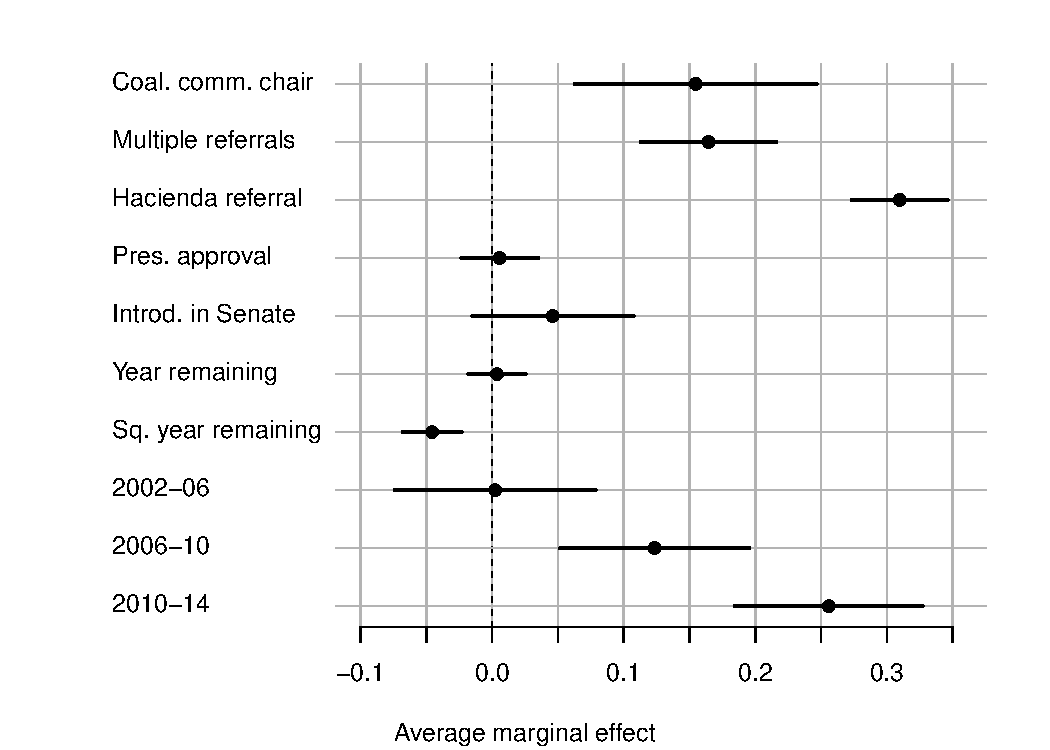
\includegraphics[width=.8\columnwidth]{../graphs/avgMgEffects.pdf}
\end{figure}

Figure \ref{F:avgMg} reports changes in the average predicted probability of an urgent bill associated with unit changes in model 3's explanatory variables (all other regressors at their mean value). This is a convenient way to translate logit regression coefficients into interpretable quantities. A report from a committee with a coalition chair experiences a .03 hike (and a .013 standard error) in the likelihood of getting a closed rule in the floor compared to a report by an opposition-chaired committee. While paling compared to the average marginal effects of \emph{Member bill} ($-.21$), \emph{Hacienda referral} (.12), or even \emph{Multiple referrals} (.06), there is no statistical evidence to reject our Hypothesis 2.  

The large effects of Hacienda and multiple referrals deserves comment. When spending gets in the way in Chile, restrictive rules are the norm. Recall that multiple referrals exclude the finance committee, so there is an independent effect of bills with jurisdictional overlaps worth investigating further. And the finance committee was always chaired by a coalition member, but with the exception of the 1998 to 2000 period, never by a co-partisan of the president. This may explain the borderline significance of our key variable in model 1. 

%Two alternative specifications ... With the exception of \emph{Senate minority}, gaining in size and achieving .1-level significance, estimate changes are negligible. The change attests that the 2010--14 Legislature, with presidential minority status throughout (the 1998--2002 had short lapses only) experienced bigger inter-chamber differences in urgency incidence. The simpler urgency models are quite robust. 

%The strategic environment controls get mixed results. Neither coefficient for \emph{Pres.~Approval} nor \emph{Senate minority} achieved statistical significance. But \emph{Introduced in Senate} did. Bills successfully passing the upper chamber before moving to the Cámara were likelier to get urgent status, and the effect is significant at the .006 level. Proposals initiated in the Senate, where the opposition was systematically larger (and at times controlled the chamber) were, other things constant, also likelier urgency targets. Note also this coefficient's sizable hike from model 1 to model 2, gaining about a third in size while other coefficients did not change when controls for member-bill sponsorship are added. The lower initiation of mix-member bills in the Senate, as opposed to the Cámara (a $-.34$ correlation between \emph{Introduced in Senate} and \emph{Member bill, mix-sponsored}) masks a portion of the effect when sponsorship controls are omitted. 

%Both time trend variables returned significant coefficients. Other things constant, bills were likelier to become urgent earlier in the term and earlier in the legislative year. The apparent contradiction of the patterns in Figure \ref{f:depvarHistog} is explained by the distinction of non-original urgency messages---where most of the temporal trend is manifest---which is disregarded by the dichotomous measure of the urgency analyzed here. 

Another control worth highlighting is \emph{Senate majority} (the other strategic environment variable, presidential approval, is insignificant). Bills successfully passing the upper chamber before moving to the Cámara were likelier to get urgent status (the average marginal effect is .02 and significant). Proposals initiated in the Senate, where the opposition was systematically larger and at times in control were, other things constant, also likelier urgency targets. This is consistent with a view that legislative compromises needed to clear the higher Senate hurdle were likelier to require protection against floor amendments, even after controlling for Hacienda committee referral. 

\begin{figure}
  \centering
    \caption{Probability of urgent bill consideration. Predictions are from from model 3 letting \emph{Year remaining} vary in full range, with 95-percent confidence bands. Other variables set at the following values: $\text{\emph{Multiple referrals}}=0$, $\text{\emph{Hacienda referral}}=1$, \emph{Pres.~approval} at its median, $\text{\emph{Introd.~in~Senate}}=0$, and $\text{\emph{2006-10}}=1$.}\label{F:sims}
    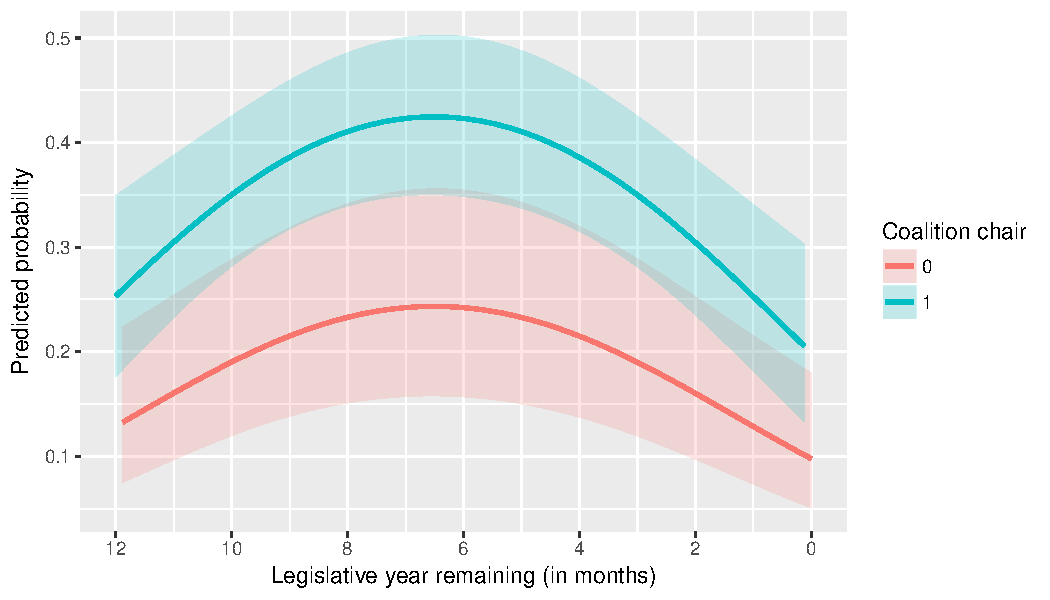
\includegraphics[width=.75\columnwidth]{../graphs/predictedPr.pdf}
\end{figure}

Finally, there are time trends in urgency authority usage that simulations reveal neatly. Figure \ref{F:sims} portrays the predicted probability that a bill gets urgent status throughout the legislative year. Regressors in model 3 are held constant to simulate a bill the executive sent to the Cámara in the 2010--14 Legislature and referred to Hacienda and just one standing committee. The president's approval is set to the median throughout the period. The inverted-U shape shows how urgency probability, predicted at almost .8 for coalition-chaired committees, and .7 for the rest at the start, becomes likelier in the first half of the legislative year. By the second quarter (June--August), the probability is at its maximum, 10 percent up since March. It then experiences a sharp drop, ending the austral Summer break at .7 for coalition-chaired committees, and .6 for others. 

It is clear that much uncertainty surrounds the predictions. If the signal of a coalition committee chair on urgency likelihood is statistically significant, the noise in the data remains important relative to the model's prediction ability. The 95-percent confidence bands of predicted probabilities in red (for a coalition committee chair) and blue (not) have substantial overlap. There remains a good deal of heterogeneity among bills reported to opposition-chaired committees that calls for refinements in our empirical model. 

\ges{Eric, yo creo que el overlap de confidence intervals no significa que no tienen efecto.  Es mas not tiene mucho que ver, podria ser que sí, podria ser que no. Sacaste los average marginal effect? Otherwise I can do that for next time}
\emm{Ahora sí los he incluido. He matizado el último párrafo.}

\section{Discussion}

Since the late Nineteenth Century, restrictive rules are the domain of the Rules committee in the U.S.\ House \citep{denhartog.2004phd,cox.mccubbins.2005,sin.2014}. However, it is the president who has possession of this key legislative prerogative in Chile. The executive branch decides which bills go to the floor with a closed rule. 

In this paper we elaborated some implications of this peculiar, inter-branch institutional arrangement. Theoretically, we found that when the committee chair's preferences are closer to those of the President, then the probabilities that bills will be labeled as urgent increases. That is, committee chairs negotiate directly with the president the bill they want to see enacted.  When this is the case, the President imposes a closed rule on it, and the bill is not modified in the floor.  In other words, this institutional tool increases cooperation between branches. Committee chair and President commit to a deal that cannot be undone because it is protected by an urgent label.


\emm{Convendrá elaborar la relevancia de que la retrictive rule esté en manos del presidente. ¿Por qué no retienen esa facultad los legisladores?}

%% McCox 2nd Ed leviathan, fn 5 p. 214: ``Congressional Quarterly (1994 <-- 19nov, 3326) describes the role played by the modern Rules committee: The Rules committee is the gatekeeper to the House floor. It has a unique role and function, determining how and whether a major bill will be considered on the floor, and which amendments and motions will be allowed. This gives the committee considerable power in shaping the legislative agenda and makes it the arbiter of frequent turf fights between other committees.''  



%Yet inspection of recent urgency message incidence reveals a strikingly high frequency: one of every five bills in Congress received some form of executive urgency at some stage (and often at several stages) of the legislative process; and more than two-thirds of executive proposals did. Adding a layer to the puzzle, Congress in fact complied with a significant number of urgency messages. Why would presidents resort so remarkably frequently to the institutionally inconsequential urgency authority? And why would legislators comply so often with empty executive threats?

\section{Appendix}

\subsection{Dichotomous variables}

\begin{tabular}{llrrr}
 Variable                          & Def &       =0 &       =1 & Total  \\ \hline
\emph{Urgent bill} (Dep.~Var.)     &     &    5,932 &    1,055 &6,987 \\
                                   &     &   .849   &   .151   &   1  \\
\emph{Co-partisan comm.~chair}     &     &    4,537 &    2,450 &6,987 \\
                                   &     &   .649   &   .351   &   1  \\
\emph{Multiple referrals}          &     &    5,342 &    1,645 &6,987 \\
                                   &     &   .765   &   .235   &   1  \\
\emph{Member bill}                 &     &    1,461 &    5,526 &6,987 \\
                                   &     &   .209   &   .791   &   1  \\
\emph{Member bill, opp.-sp.}       &     &    4,813 &    2,174 &6,987 \\
                                   &     &   .689   &   .311   &   1  \\
\emph{Member bill, mix-sp.}        &     &    5,326 &    1,661 &6,987 \\
                                   &     &   .762   &   .238   &   1  \\
\emph{Member bill, pres.~coal-sp.} &     &    5,296 &    1,691 &6,987 \\
                                   &     &   .758   &   .242   &   1  \\
\emph{Hacienda referral}           &     &    6,120 &      867 &6,987 \\
                                   &     &   .876   &   .124   &   1  \\
\emph{Senate minority}             &     &    4,302 &    2,685 &6,987 \\
                                   &     &   .616   &   .384   &   1  \\
\emph{Introduced in Senate}        &     &    5,080 &    1,907 &6,987 \\
                                   &     &   .727   &   .273   &   1  \\
\emph{Relax deadlines}             &     &    4,783 &    2,204 &6,987 \\
                                   &     &   .685   &   .315   &   1  \\
\end{tabular}

\subsection{Continuous variables}

\begin{tabular}{llrrrrrrr}
               Var.  & Def. &  Min.&  Q1 & Med. & Mean &  Q3  &  Max. &   sd \\ \hline
\emph{Pres.~term}    &      &  0   &  29 & 54   & 51.8 & 75   & 100   & 27.6 \\
\emph{Year remaining}&      &  0   &  31 & 53   & 53.2 & 75   & 100   & 26.4 \\
\emph{Pres.~approval}&      &-39.2 & -12 &  4.9 &  6.1 & 19.8 &  66.3 & 24   \\
\end{tabular}


%% TODO ESTO VIENE DE ANTERIOR VERSION... DESCOMENTAR PARA VER QUE ES RESCATABLE

%% \section{The received wisdom}

%% \begin{center}
%% \singlespacing
%% [U]rgency powers... can have dramatic effects on executive-legislative \\ 
%% relations, legislative organization, and the policy process more generally\\ 
%% ---\citet[][:438]{morgenstern.2002b}
%% \end{center}
%% \onehalfspacing

%% %\citeauthor{carey.shugart.1998a}'s \citeyearpar{carey.shugart.1998a} monograph on executive unilateral powers does not discuss it. \citeauthor{londregan.2000a}'s \citeyearpar{londregan.2000a} study of legislative institutions in the Chilean Senate does not include the urgency authority in the index. 

%% \noindent Scholars have paid little attention to the urgency authority. \citeauthor{shugart.carey.1992}'s \citeyearpar{shugart.carey.1992} seminal monograph does not include it when computing the index of presidents' legislative powers. And while not addressing it directly either, \citeauthor{carey.shugart.1998a}'s \citeyearpar{carey.shugart.1998a} discussion of the delegation of unilateral authority to the executive offers clues of the logic behind the institution. Informational and valence asymmetries between Latin American executive and legislative branches create incentives for such delegation. Delays to reach agreement in assemblies offer further incentives by diminishing the value of policy \citep{baron.ferejohn.1989}, so rather than delegate proposal power within the chamber, legislators may find it preferable to let the president set the agenda. 

%% %\citet{siavelis.2002} is the first study to cover the urgency authority. He hypothesized urgencies' game-changer potential. His study of Chilean executive-legislative covers the first post-transition presidency revealed just how very frequently urgency messages were issued: slightly more than one-third of proposals in Congress received some form of urgency, and about 9 out of 10 of urgent bills were executive-initiated. Guided by semantics, analysis sought to discover if urgent bills, in fact, circulated the steps of the legislative process faster than the rest, and whether urgency status also increased the likelihood of bill passage. The study found mixed evidence. Among executive bills, consideration of urgent ones had somewhat shorter duration than the rest (medians of 134 and 160 days, respectively), but no palpable difference in success rates is appreciated (64 and 63 percent, respectively). 

%% \citet{siavelis.2002} is the only systematic study of the urgency authority we are aware of. Like Morgenstern's quote, he hypothesized the urgency power's game-changer potential. His study of Chilean executive-legislative in the first post-transition administration revealed the amazing frequency with which urgency messages were issued by President Aylwin: slightly more than one-third of proposals in Congress received some form of urgency, and about 9 out of 10 of urgent bills were executive-initiated. Guided by semantics, he also sought to discover if ``urgent'' bills, in fact, circulated the steps of the legislative process faster than the rest, and whether urgency status increased the likelihood of bill passage. The study found mixed evidence at best. Among executive bills, consideration of those urgent had somewhat shorter duration than the rest (medians of 134 and 160 days, respectively), but no palpable difference in success rates is appreciated (64 and 63 percent, respectively). 

%% The negative finding may bear relation to three elements. In their study of budgetary congressional oversight of the executive, \citet{berrios.gamboa.fiscChile.2006} warn against overstating the Chilean urgency authority's importance, as non-compliance entails no penalty for Congress---the next section develops this argument. While this may explain the lack of effects, it begs the question of why the president resorted so frequently to an authority that seems inconsequential. In other words, why make so many empty threats?

%% Another is a failure to control for urgency degrees---elaborated in section 3---in the analysis. \citeauthor{aleman.navia.UrgChi.2009}'s \citeyearpar{aleman.navia.UrgChi.2009} systematic study of executive success in Congress in three post-transition presidencies finds some of the evidence sought by Siavelis. Controlling for bill characteristics (such as key policy domains, the chamber where the bill originated, the government's seat margin, and presidential agenda size), urgency degrees had quite different effects in passage. Higher degrees significantly associate with better probability of executive success, but the lower made no statistical difference. Since, as will be seen, low-degree urgencies were much more prevalent, conflating them washes off the effect of the higher-degree. 

%% % longer review of aleman and navia
%% %\citeauthor{aleman.navia.UrgChi.2009}'s \citeyearpar{aleman.navia.UrgChi.2009} systematic study of executive success in Congress in three post-transition presidencies also inspects Chile's urgency authority. Among controls, their equation includes urgency authority usage in the right side. The unit is the individual bill, and the size of the executive agenda varies substantially over the years. Variation is quantitative  (Congress received about 150 presidential bills in each of the first 6 years after 1990, a numbrer that dropped to about 70 in the next 6 years, then climbed to about 100 in the final 4 years of their series) and qualitative, presidents manifesting different propensities to aim at constitutional reform. Of direct relevance are the findings on urgencies. Controlling for key policy domains, chamber of origin, seat margins, and presidential approval, and clustering errors by legislative year, different prioritization reveal quite different effects in passage. `Act now' and `2-week' notices significantly increased the probability of bill passage, but not `one month' notices. 

%% Finally, selection bias is an obstacle to measure urgency authority effects. Presidents, behaving strategically, are likely to target for urgency proposals that are markedly different from the rest in important ways, so the set of bills receiveing urgent status is not random. Like the Siavelis and Alemán-Navia studies, we recognize the endogeneity problem that arises but does not confront it methodologically. Until a more subtle identification design is proposed, findings must be taken with a grain of salt. The systematic study of the urgency authority in Chile that follows should contribute to pave the way to a solution. 

%% %If presidents, behaving strategically, were to target for urgency proposals that are markedly different from the rest in important ways, a problem of endogeneity arises. Classify proposals based on how difficult passage is expected: easy, hard, and impossible. If left on their own, the easy proposals would be approved faster, the hard slower, the impossible never. A strategic president should concentrate the urgency authority in the hard group, leaving easy proposals mostly on their own, while abandoning the hopeless group of impossible proposals, that will not be observed. As a consequence, comparing

%% %The relevant quantity of interest is whether the use of the urgency authority affects bill passage (success, speed, amendments, and so forth) compared to the same bill with no urgency attached. The fundamental problem of causal inference is immediately evident. The executive presumably targets bills for urgency strategically, so that the selection mechanism cannot be assumed random. If, for example, more complex and divisive legislation takes longer, is likelier to fail and likelier to be tagged urgent, separating effects requires more subtle methods than used up to now.


%% \section{Variable urgency degrees}
%% \begin{center}
%% Presidential power is the power to persuade ---Neustadt\footnote{\citet[][:11]{neustadt.1990}}
%% \end{center}


%% Vagueness surrounds key aspects of the urgency authority. When a 30-day limit is set, for instance, no indication is given of whether those are calendar, business, or session days. I treat the messages in weeks rather than days given imprecision (and, when coding deadlines in the empirical sections below, rely on business days, as \citet[][:285]{sotoCongChile2015} suggests). More important, no formal reversionary course of action is defined, and no hint of rulings by the Constitutional Tribunal filling in the institutional void could be found. As seen in the previous section, I interpret indeterminacy as reversion to the status quo with no effect on the voting schedule.


%% %Urgency type frequency, in fact, reveals a tendency to rely less often on more urgent messages (descriptive data is presented in the next section). `Act now' notices were roughly 3 to 5 times less frequent than `two week' ones in a recent 16-year period. The frequency differential between `two week' and `one month' notices is less sharp, but a tendency is distinguishable. 


%% \section{The data}


%% % \begin{table}
%% % \begin{center}
%% % \begin{tabular}{rrr}
%% % Number of &      Bill &     \\
%% % messages  & frequency &  ~~~~~~~~\% \\ \hline
%% % %None              &  5635     &     \\
%% % 1                 &  214      &  \emph{16}   \\
%% % 2                 &  242      &  \emph{18}   \\
%% % 3                 &  145      &  \emph{11}   \\
%% % 4                 &  115      &  \emph{8}    \\
%% % 5                 &  104      &  \emph{8}    \\
%% % 6-10              &  236      &  \emph{17}   \\
%% % 11-20             &  183      &  \emph{13}   \\
%% % 21-40             &  99       &  \emph{7}    \\
%% % 41-71             &  24       &  \emph{2}    \\
%% % Total             & 1,362     & \emph{100}   \\ \hline
%% % \end{tabular}
%% % \caption{Urgent bills classified by number of urgency messages received}\label{T:billFreqByNurg}
%% % \end{center}
%% % \end{table}

%% % Other interesting patterns in urgency authority usage are discernible in bill histories. Assessing how large the subset of bills receiving one or more urgency messages is conveys a minimalist perspective of the urgency authority. As shown in table \ref{T:billFreqByNurg}, most bills in this subset (84 percent) in fact received many such messages, and a substantial portion (40 percent) received between 6 and 71 urgency messages. This raises another puzzle for research. Are presidents reiterating urgency messages because of Congressional inaction? Extending the deadline may help the president save face when legislative non-compliance is imminent. Or are presidents micro-managing select-bill consideration in committee, monitoring a report's progress and then sending recommendations in the message extending the deadline? The source indicates the arrival of presidential messages but does not include their actual contents, nor those of committee reports. Archival research to retrieve those documents would do wonders in answering these questions. 

%% %A bicameral process operating on a single-round navette \citep{tsebelis.money.1997}---bills migrate from originating to revising chamber, back to originating if amended, and finally to conference if inter-cameral differences persist---offers, at most, four clear instances for repeated urgency authority use. Yet, as table \ref{T:billFreqByNurg} reports, nearly half of urgent bills (47 percent) received five messages or more. A handful of bills received several dozen messages! 

%% \begin{figure}
%% \begin{center}
%%  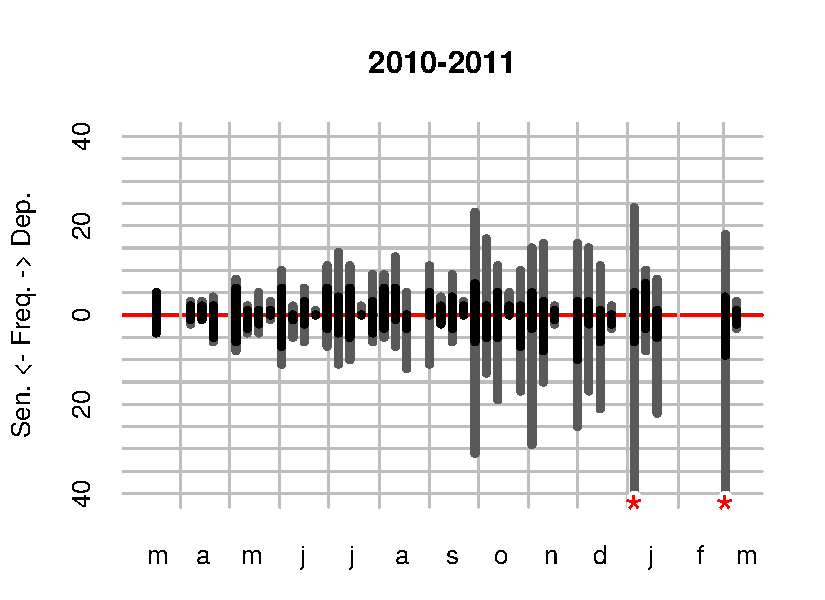
\includegraphics[width=.65\columnwidth]{../graphs/urgenciasHistog2010.pdf}
%% \begin{tabular}{cccc}
%%     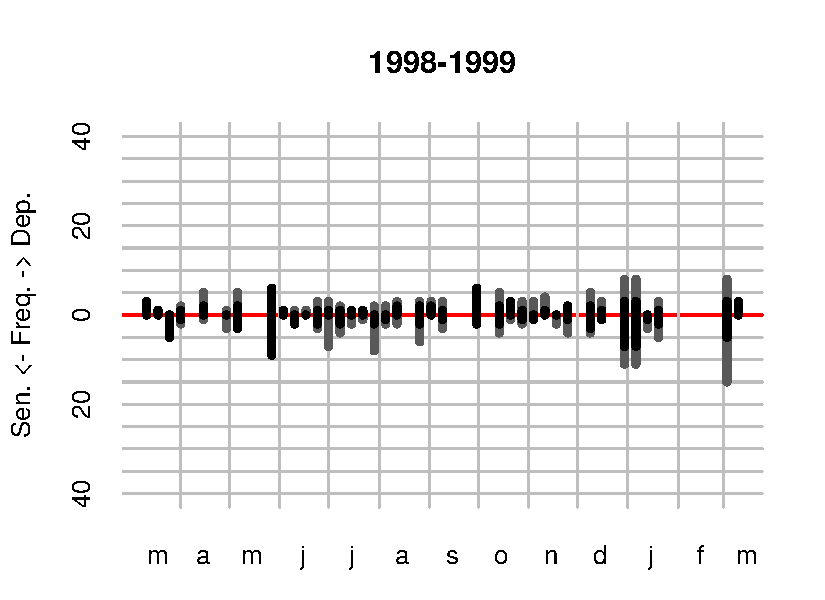
\includegraphics[width=.22\columnwidth]{../graphs/urgenciasHistog1998.pdf} &
%%     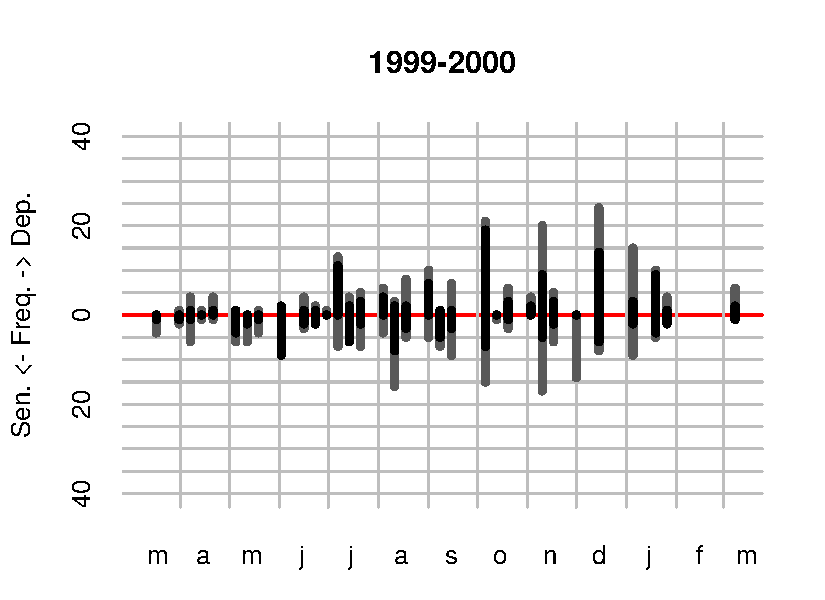
\includegraphics[width=.22\columnwidth]{../graphs/urgenciasHistog1999.pdf} &
%%     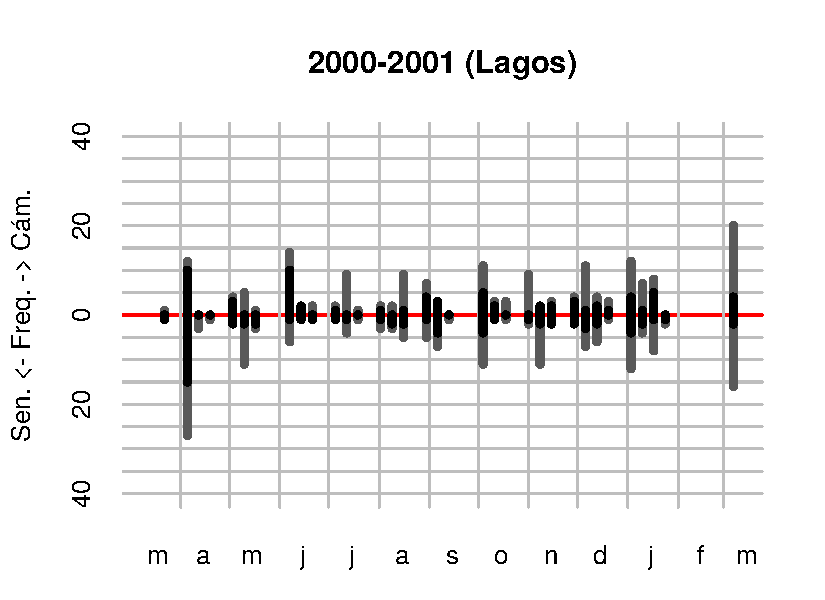
\includegraphics[width=.22\columnwidth]{../graphs/urgenciasHistog2000.pdf} &
%%     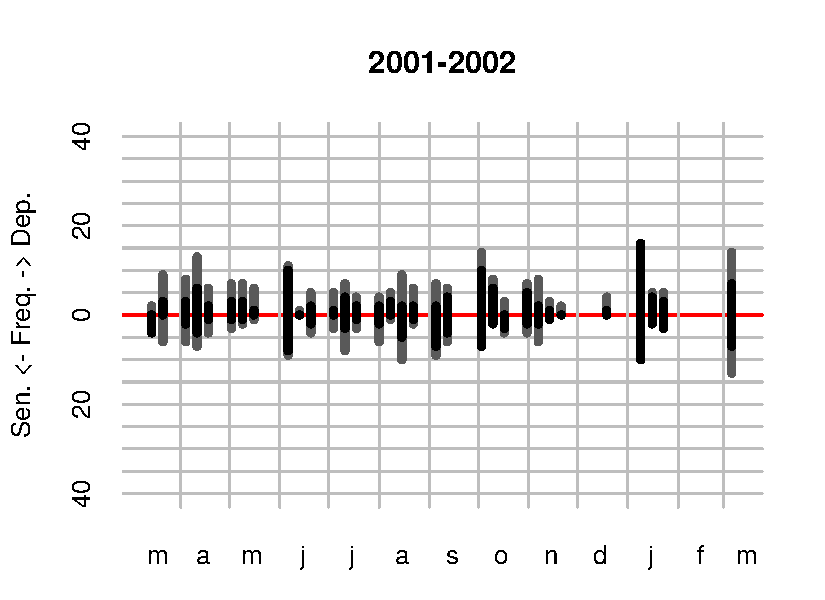
\includegraphics[width=.22\columnwidth]{../graphs/urgenciasHistog2001.pdf} \\
%%     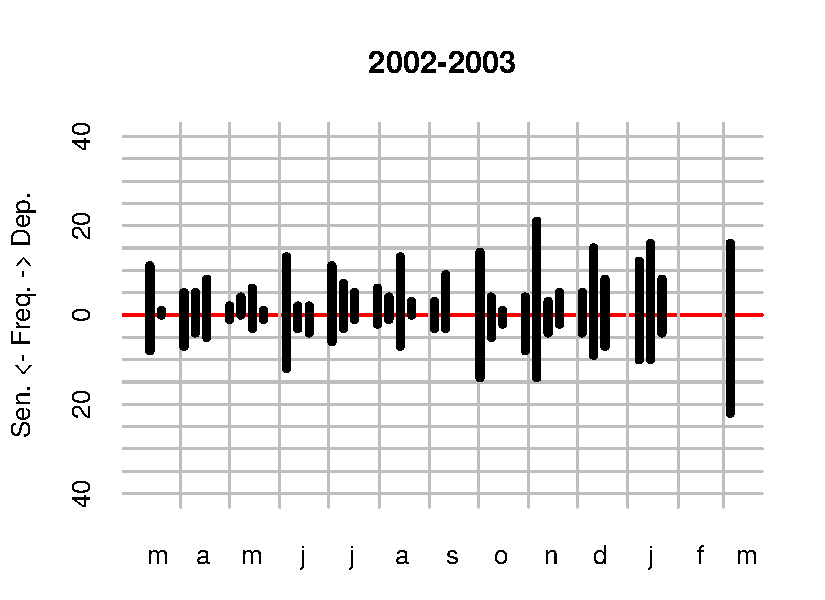
\includegraphics[width=.22\columnwidth]{../graphs/urgenciasHistog2002.pdf} &
%%     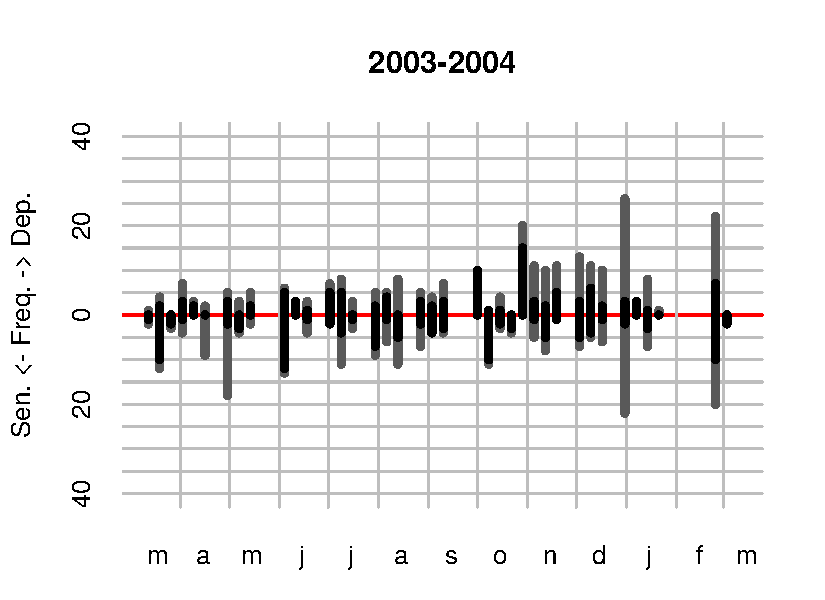
\includegraphics[width=.22\columnwidth]{../graphs/urgenciasHistog2003.pdf} &
%%     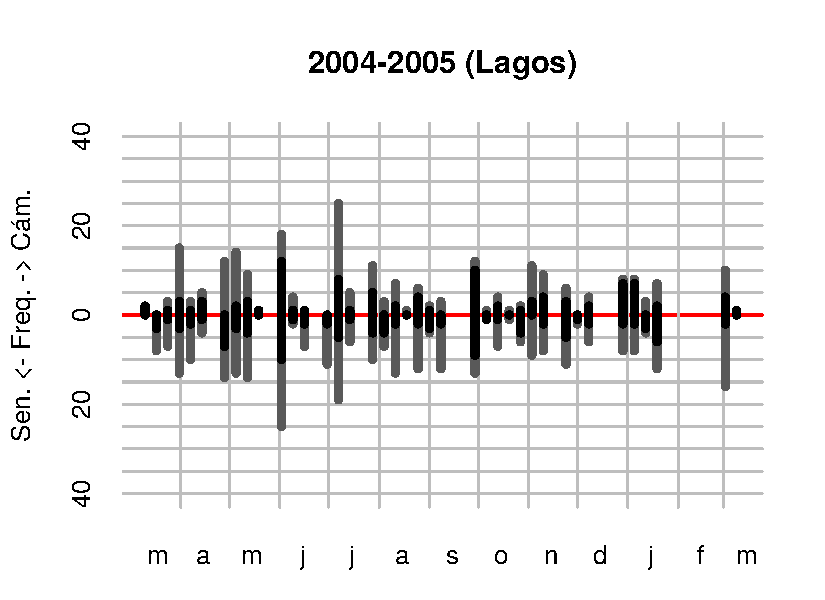
\includegraphics[width=.22\columnwidth]{../graphs/urgenciasHistog2004.pdf} &
%%     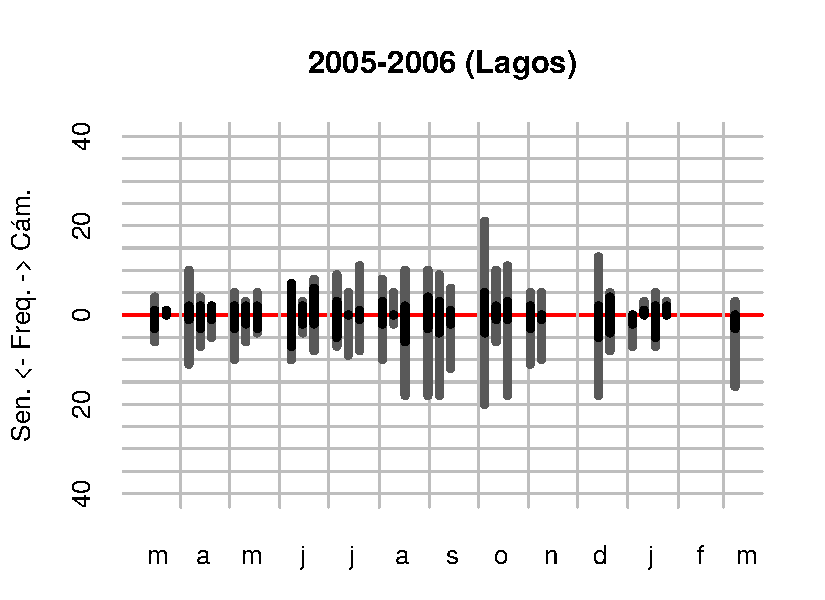
\includegraphics[width=.22\columnwidth]{../graphs/urgenciasHistog2005.pdf} \\
%%     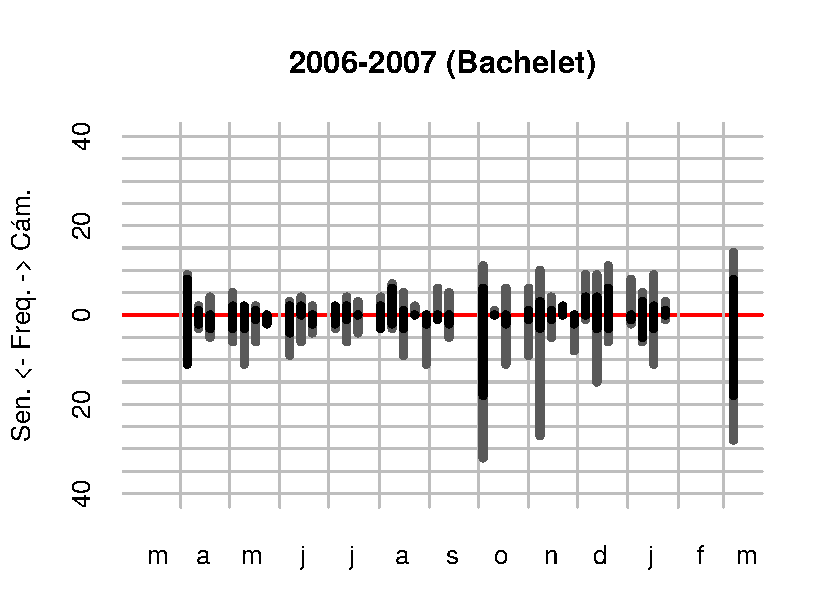
\includegraphics[width=.22\columnwidth]{../graphs/urgenciasHistog2006.pdf} &
%%     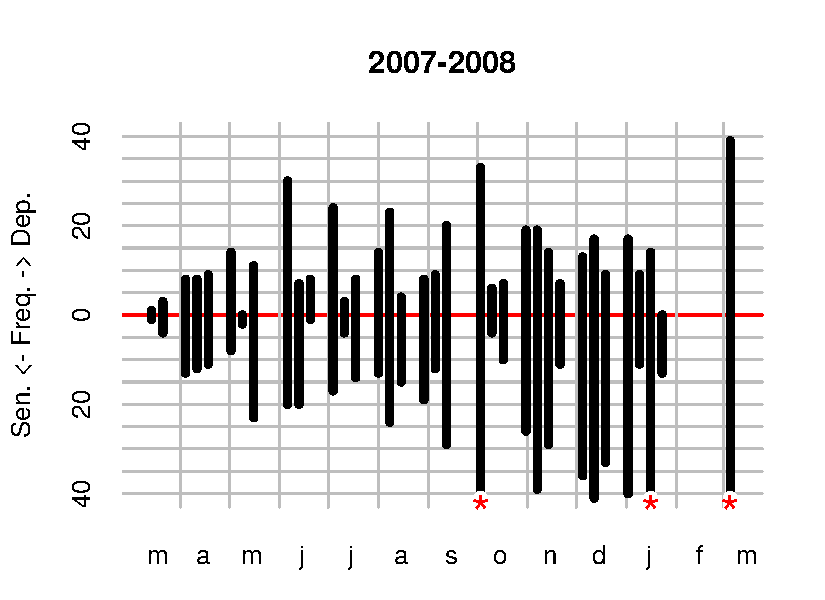
\includegraphics[width=.22\columnwidth]{../graphs/urgenciasHistog2007.pdf} &
%%     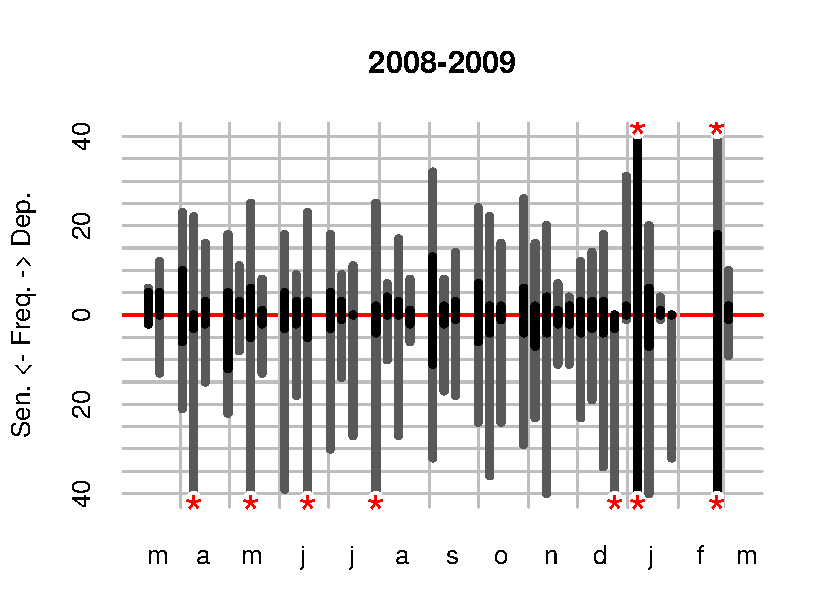
\includegraphics[width=.22\columnwidth]{../graphs/urgenciasHistog2008.pdf} &
%%     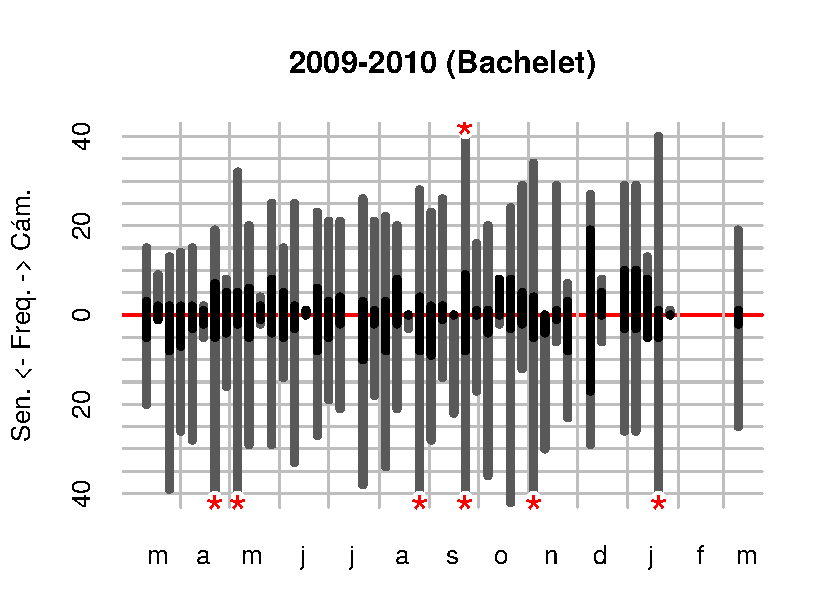
\includegraphics[width=.22\columnwidth]{../graphs/urgenciasHistog2009.pdf} \\
%%     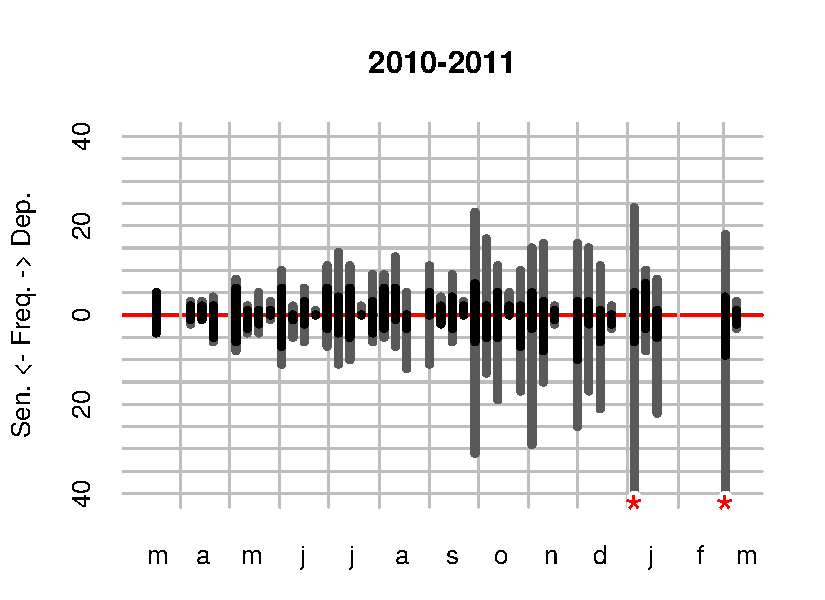
\includegraphics[width=.22\columnwidth]{../graphs/urgenciasHistog2010.pdf} &
%%     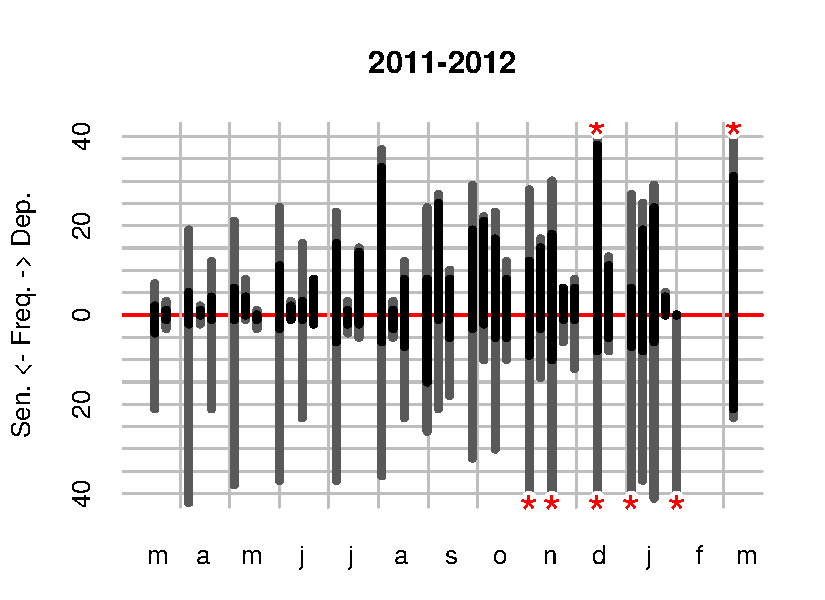
\includegraphics[width=.22\columnwidth]{../graphs/urgenciasHistog2011.pdf} &
%%     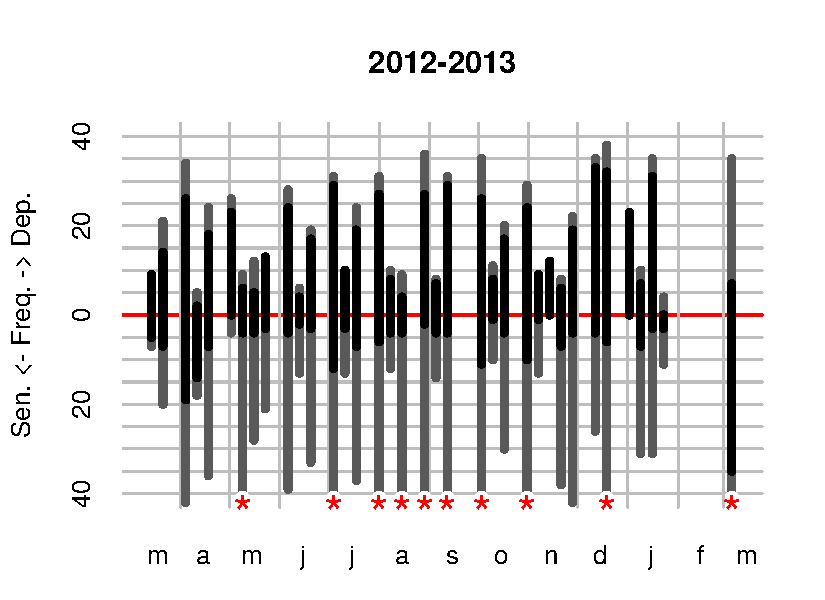
\includegraphics[width=.22\columnwidth]{../graphs/urgenciasHistog2012.pdf} &
%%     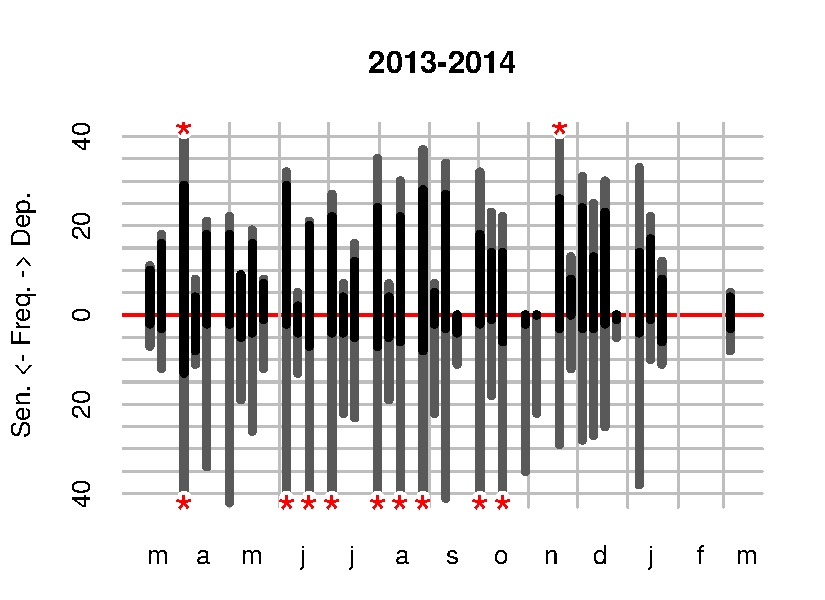
\includegraphics[width=.22\columnwidth]{../graphs/urgenciasHistog2013.pdf} \\
%% \end{tabular}
%%   \caption{Weekly urgency messages by legislative year. Cámara histogram above, Senate below the zero line. Black portion of bars indicates original urgencies, gray portion indicate deadline changes and urgency withdrawals. Asterisk atop column indicates off-the-chart urgency message frequency.}\label{f:depvarHistog}
%% \end{center}
%% \end{figure}

%% % \begin{figure}
%% % \begin{center}
%% %     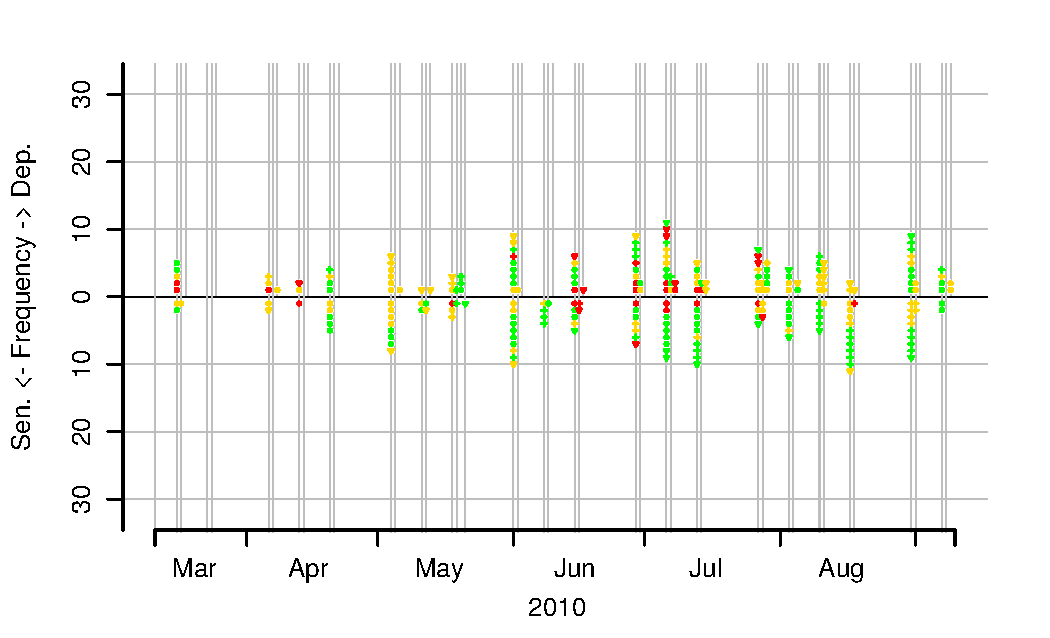
\includegraphics[width=\columnwidth]{../graphs/urgencias2010-1.pdf} \\
%% %     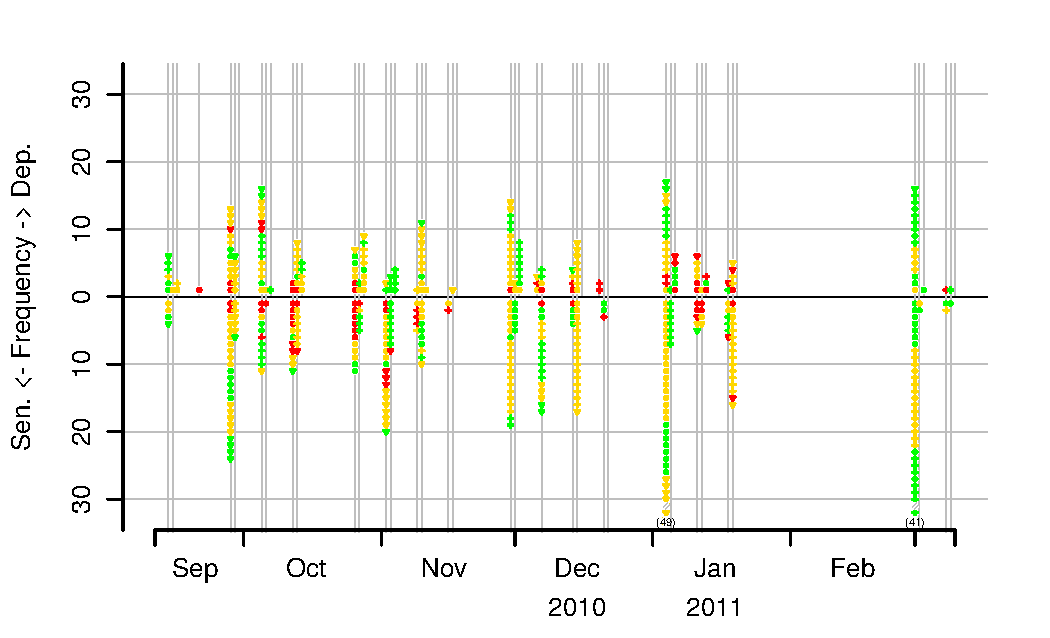
\includegraphics[width=\columnwidth]{../graphs/urgencias2010-2.pdf} 
%% %   \caption{Urgency messages in legislative year 2010--11. Diputados and Senate data above and below the zero line, respectively. Vertical gray lines indicate that a session took place. One point for each urgency message, a circle for a newly declared urgent bill, a plus sign for an urgent bill with new deadline, a triangle for an urgency withdrawn. Point color indicates the urgency type, red for `act now', yellow for `two week', green for `one month'. Parentheses atop columns indicate off-the-chart urgency message frequency.}\label{f:depvar}
%% % \end{center}
%% % \end{figure}

%% Chains offer a better perspective of the evolution of urgency usage than sheer messages. The 170 percent message surge between the 2002--06 and 2006--10 Legislatures was, in fact, due to declaring 90 percent more legislation urgent, the rest attributable to substantially longer chains (4.2 links on average, up from 3). The 2010--14 hike is mostly due to longer chains (4.7 links on average), as the chain frequency increase was negligible. Plotting weekly urgency messages in the period, as Figure \ref{f:depvarHistog} does, reveals how original urgency incidence changed little over the years, unlike non-original message incidence. Each panel in the figure (one of which is zoomed above to provide detail) reports one legislative year as two super-imposed histograms, one for Cámara and one for Senate messages (both positive scales, red asterisks marking off-the-chart counts). The black portion of columns count original urgency messages, the gray count deadline changes and withdrawals. Note how black central segments had some tendency to grow in both chambers from year to year. But that change looks minute compared to how the gray fringes expanded. Urgency-wise, Presidents Bachelet (2006--10) and Piñera (2010--14) had relatively quiet first years in office, using the authority much more often after the second, and especially after the third year. Piñera's more insistent messages to the Senate than the Cámara, as seen in the red star asymmetry, coincided with a lack of majority in the chamber. 

%% \begin{table}
%% \begin{center}
%% %\begin{small}
%% \begin{tabular}{lrrrrrrrr}
%%                          &  \mc{8}{c}{Percent Concertación sponsors} \\
%% Urgency raised by        &  0\%      &  1--25    &  26--50    &  51--75    &  76--99    &  100\%      &  All         &  N \\ \hline
%% Concertación presidents& \emph{21} & \emph{3}  & \emph{10}  & \emph{15}  & \emph{13}  & \emph{39}   &  \emph{100}  &  228 \\
%% Right president          & \emph{26} & \emph{4}  & \emph{18}  & \emph{12}  & \emph{12}  & \emph{26}   &  \emph{100}  &  121 \\
%% \end{tabular}
%% \caption{Sponsorship of urgent member proposals. Entries are relative frequencies of Concertación sponsors among bills declared urgent by presidents elected by list given in row. The first entry reports that 21 percent of bills declared urgent by a Concertación president had not a single co-sponsor elected by that list; and so forth.}\label{T:sponsorsOfUrgBills}
%% %\end{small}
%% \end{center}
%% \end{table}

%% % ``Para evitar entorpecer el funcionamiento de Congreso, el Ejecutivo procura no tener, al mismo tiempo, más de 10 proyectos con urgencia en cada una de las Cámaras (entrevista Carmona)'' (fn.~25) Carmona citado en berrios gamboa

%% Also plain in figure \ref{f:depvarHistog} is the time scarcity problem. If the urgency authority were consequential, the abundance of messages would pose a genuine scheduling problem for members and their legislative parties. Not taking the February Summer break into account (when Congress rarely convenes), the Cámara in the median legislative year had just 4 weeks free of original urgency messages, and none free of urgency messages of either type. Saturating the agenda with urgent executive bills inevitably plunders scheduling time to consider members' pet projects.\footnote{\citet{berrios.gamboa.fiscChile.2006} quote the executive's legal chief of staff describing a general goal in the Executive branch to have, at most, ten urgent projects in each chamber at once and thus ``prevent blundering congressional work (\emph{evitar entorpecer el funcionamiento de Congreso})'' (fn.~25). It is an optimistic assessment of presidential self-restraint, to say the least. If the urgency authority were consequential, presidents who have taken the chamber's schedule hostage might be a better analogy than self-restraint.} The president may be taking the legislative schedule hostage \citep[cf.][]{cox.mccubbins.1994,williamson.1975}. In such circumstances, the urgency authority is another asset for vote-buying, presidents freeing up scheduling time or even granting members' projects urgent status in exchange for support for difficult proposals. The evidencein table \ref{T:sponsorsOfUrgBills} is consistent with this conjecture: controlling for the percentage of signatures by legislators belonging to Concertación parties in the proposal reveals that presidents often granted urgent status to opposition bills. Of member bills declared urgent by Concertación presidents (1998--2010), 21 percent fell in this category, and 26 percent by the right-of-center administration that followed (2010--2014). This bonding perspective of scheduling is a promising line of research of executive-legislative negotiation. 

%% \section{Urgency chains}

%% Urgency authority predictors aide the interpretation of the next pieces of analysis. Units here are not individual bills but urgency instances, in search for correlates in the legislation they target. The previous section ignored urgency reiteration, a striking pattern in the data. This section isolates urgency chains in search for one observable consequences in the legislative process. If the urgency authority were consequential, it should prompt action in the chamber where the bill awaited consideration. Moreover, the action should happen within the deadline established by the president. 

%% Several actions might follow an urgency call: the bill is marked in committee; one or more committee reports (called \emph{informes} in Chile) are drafted and adopted; the bill is reported, with possible revisions or even a negative advise, to the floor; a positively-reported bill is scheduled in the Order (\emph{Orden del Día}); the plenary considers, possibly amends, and eventually votes the bill's passage; and possibly others. Analysis here focuses on committee reports. Unlike some of the steps listed, reports are observable in the bill histories collected. If report contents are, unfortunately, unavailable in the data, the drafting committee(s) and report date(s) are included. Since urgency messages are also dated, synchronicity can be verified systematically.  

%% Committee reports are a good choice to search for urgency authority effects because only exceptional cases should not get one. Unless the floor votes an exception to the rules unanimously, every bill in Chile is referred to a standing or special committee upon first introduction to each chamber. Another exception are bills previously reported at the time the urgency call is made. A last exception are bills discharged from committee for direct floor consideration. No explicit discharge procedure could be found in the congressional standing orders, but presumably it is the same---unanimous consent---to consider a bill without prior committee referral. There is no record in the data to verify it, but the presumption is that such exceptions are rare. At any rate, exceptions play against detecting ripples caused by the urgency authority.

%% One hypothesis of consequential urgency authority tested is that raising an urgency prompts a committee report. A finer hypothesis involves the chronology of events: if the urgency authority were consequential, bill reporting should occur \emph{before} the given deadline expires. Because the terms of the urgency were modified so often in the period, chains---not individual messages---are considered for analysis, expecting reports on or before the chain's final deadline. Rejecting hypotheses weighs against consequential urgency authority, committees retaining the potential as formidable gatekeepers in their policy jurisdiction---failure to draft a report prevents the proposal from progressing in the legislative process \citep{cox.mccubbins.1993,fenno.1973,shepsle.weingast.1987}. 

%% %Due to the frequency with which deadlines are adjusted, expecting a timely reports for every message is unreasonable, even if the urgency authority were consequential. The relevant units are therefore not urgency messages but urgency chains: reports should antedate the final deadline set by a chain of messages. 

%% %This section analyzes bill histories to detect whether or not reports follow urgency messages in the Cámara de Diputados, and whether or not this occurs in a timely manner. Failure to observe the report is evidence of inconsequential urgency authority.  

%% As mentioned, the Hacienda committee has special status in the Chilean Congress and deserves attention. Unlike other committees, Hacienda has jurisdiction over \emph{every} bill authorizing spending in any domain. Moreover, the unanimous exception rule is inapplicable to Hacienda bills, which \emph{must} be reported to be considered in the floor.\footnote{Standing rules (Ley orgánica del Congreso) arts.\ 17 and 21.} So, for instance, a proposal restricting labor benefits to certain state health workers at the municipal level was referred to both the Public Health and Hacienda committees because a small appropriation for verification by the Labor Bureau was required. Hacienda committee members, working in tandem with Finance Ministry staff \citep{aleman.navia.UrgChi.2009}, may or may not appropriate funds from the budget in their report to the floor. Not unlike the Appropriations and Rules committees in the U.S.\ House, Hacienda has the status of a control committee, a key asset for agenda power \citep{kiewiet.mccubbins.1991}. Because Hacienda referral is mandatory, only previously reported bills would not get a Hacienda report following an urgency. 

%% The assessment of predictors of timely committee reports analyzes the subset of chains from bills that were referred to the Hacienda committee separately from the full set of chains in the period. The dependent variable equals 1 if a report (an Hacienda report in the chain subset) is observed on or before the deadline set by the final message in the chain (business days used for computation); equals 0 otherwise. The multivariate analysis includes predictors in the previous section (defined over chains instead of bills), minus Hacienda referral---a bill trait is controlled differently here---and presidential approval.\footnote{Including \emph{Pres.~approval} returns a statistically insignificant coefficient and produces negligible changes in other predictors.} Also in the right side are indicators for original urgency message types. \emph{2~week~notice} and \emph{1~month~notice} are mutually-exclusive dummies equal 1 if the first, or only, message in the chain is of the said type, respectively, and 0 otherwise. The omitted category are act now messages, which serve as baseline for coefficient interpretation. There are also indicators for reiterated messages. \emph{Change~deadline} equals 1 if at least one message extending or cutting short the original deadline is chained to the first urgency message; equals 0 otherwise. And \emph{Withdraw~urgency} equals 1 if the final message in a chain dropped the bill's urgent status; equals 0 otherwise. An alternative specification with 11 mutually-exclusive dummies (Act now singleton; Act now with deadline modified; Act now withdrawn; and so forth) yielded essentially identical results in a much less parsimonious equation.  

%% %The predictors used in the urgency models... \emph{Senate minority} and predictors listed below in Table \ref{t:chainsRegs}) are defined for chains instead of bills: Senate minority equals 1 if the opposition had majority status when the chain started and 0 otherwise; and so forth. 

%% % \begin{table}
%% % \begin{center}
%% % \begin{tabular}{lrr}
%% %                           &  \% chains      &              \\
%% %                           &  of type with   &              \\
%% %                           &  timely         &  (N Hacien-   \\ 
%% % Message type              &  Hacienda report&  da-referred)   \\ \hline
%% % Act now singleton         &               &  \\
%% % Act now, extend           &               &  \\
%% % Act now, withdraw         &               &  \\
%% % Act now, extend, withdraw &               &  \\
%% % 2 week singleton          &               &  \\
%% % 2 week, extend            &               &  \\
%% % 2 week, withdraw          &               &  \\
%% % 2 week, extend, withdraw  &               &  \\ 
%% % 1 month singleton         &               &  \\
%% % 1 month, extend           &               &  \\
%% % 1 month, withdraw         &               &  \\
%% % 1 month, extend, withdraw &               &  \\ 
%% % All                       &               &  \\
%% % \end{tabular}
%% % \caption{Urgency messages and committee reports within deadline}
%% % \end{center}
%% % \end{table}

%% % Table created by stargazer v.5.2 by Marek Hlavac, Harvard University. E-mail: hlavac at fas.harvard.edu
%% % Date and time: Sat, Sep 12, 2015 - 10:03:41 PM
%% % Requires LaTeX packages: dcolumn 
%% \begin{sidewaystable}[!htbp] 
%% %\begin{table}[!htbp] 
%% \centering 
%% \resizebox{.9\textwidth}{!}{
%% \begin{tabular}{@{\extracolsep{0pt}} l D{.}{.}{-3} D{.}{.}{-3} D{.}{.}{-3} D{.}{.}{-3} D{.}{.}{-3} D{.}{.}{-3} D{.}{.}{-3} D{.}{.}{-3} } 
%% % \\[-1.8ex]\hline 
%% % \hline \\[-1.8ex] 
%% \hline \\[-1.8ex] 
%%  && \multicolumn{3}{c}{Hacienda report before deadline} && \multicolumn{3}{c}{Any committee report before deadline} \\ 
%% % \\[-1.8ex] & \multicolumn{3}{c}{\textit{logistic}} & \multicolumn{1}{c}{\textit{generalized linear}} & \multicolumn{3}{c}{\textit{logistic}} & \multicolumn{1}{c}{\textit{generalized linear}} \\ 
%% %  & \multicolumn{3}{c}{\textit{}} & \multicolumn{1}{c}{\textit{mixed-effects}} & \multicolumn{3}{c}{\textit{}} & \multicolumn{1}{c}{\textit{mixed-effects}} \\ 
%% \\[-1.8ex] && \multicolumn{1}{c}{(5)} & \multicolumn{1}{c}{(6)} & \multicolumn{1}{c}{(7)} && \multicolumn{1}{c}{(8)} & \multicolumn{1}{c}{(9)} & \multicolumn{1}{c}{(10)}\\ 
%% \\[-1.8ex] \hline \\[-1.8ex] 
%%  \emph{2 week} && .470^{***} & .458^{***} & .468^{***} && .661^{***} & .660^{***} & .661^{***} \\ 
%%  \emph{notice} && (.006) & (.008) & (.007) && (<.001) & (<.001) & (<.001) \\ [.75ex]
%%  \emph{1 month} && .033 & .016 & .030 && .206 & .202 & .206 \\ 
%%   \emph{notice} && (.856) & (.932) & (.867) && (.146) & (.155) & (.146) \\ [.75ex]
%%  \emph{Change} && .455^{***} & .472^{***} & .458^{***} && .388^{***} & .394^{***} & .388^{***} \\ 
%%  \emph{deadline} && (.002) & (.002) & (.002) && (.001) & (.001) & (.001) \\ [.75ex]
%%  \emph{Withdraw}  && .341^{***} & .411^{***} & .353^{**} && .168 & .193^{*} & .168 \\ 
%%  \emph{urgency} && (.010) & (.003) & (.011) && (.107) & (.074) & (.107) \\ [.75ex]
%%  \emph{Member bill}  && .190 & .129 & .179 && -1.255^{***} & -1.248^{***} & -1.255^{***} \\ 
%%  \emph{pres. coal.-sp}. && (.709) & (.800) & (.726) && (<.001) & (<.001) & (<.001) \\ [.75ex]
%%  \emph{Member bill}  && .530 & .632 & .549 && -1.088^{***} & -1.074^{***} & -1.088^{***} \\ 
%%  \emph{mix.-sponsored} && (.398) & (.315) & (.384) && (<.001) & (<.001) & (<.001) \\ [.75ex]
%%  \emph{Member bill}  && 1.057^{**} & 1.089^{**} & 1.063^{**} && -.746^{***} & -.731^{***} & -.746^{***} \\ 
%%  \emph{opp.-sponsored} && (.049) & (.043) & (.048) && (<.001) & (<.001) & (<.001) \\ [.75ex]
%%  \emph{Pres.~term}  && .275^{***} & .289^{***} & .277^{***} && .308^{***} & .315^{***} & .308^{***} \\ 
%%  \emph{remaining} && (<.001) & (<.001) & (<.001) && (<.001) & (<.001) & (<.001) \\ [.75ex]
%%  \emph{Year} && .104 & .098 & .103 && .011 & .009 & .011 \\ 
%%  \emph{remaining} && (.102) & (.122) & (.106) && (.822) & (.847) & (.822) \\ [.75ex]
%%  \emph{Chain in}  && .295^{**} & .303^{**} & .296^{**} && .472^{***} & .472^{***} & .472^{***} \\ 
%%  \emph{Senate} && (.020) & (.017) & (.020) && (<.001) & (<.001) & (<.001) \\ [.75ex]
%%  \emph{Senate}  &&  .346 &  .220 &  .324 &&  .192 &  .173 &  .192 \\ 
%%  \emph{minority} && (.248) & (.532) & (.299) && (.393) & (.516) & (.393) \\ [.75ex]
%%  \emph{Relax} && -.605^{*} & -.463 & -.589^{*} && -.088 & .080 & -.088 \\ 
%%  \emph{deadlines} && (.051) & (.468) & (.066) && (.708) & (.863) & (.708) \\ [.75ex]
%%  % 2002--06 Leg. &&  & .084 &  &&  & .051 &  \\ 
%%  %  &&  & (.721) &  &&  & (.781) &  \\ [.75ex]
%%  % 2006--10 Leg. &&  & -.310 &  &&  & -.094 &  \\ 
%%  %  &&  & (.171) &  &&  & (.592) &  \\ [.75ex]
%%  % 2010--14 Leg. &&  & -.147 &  &&  & -.187 &  \\ 
%%  %  &&  & (.839) &  &&  & (.725) &  \\ [.75ex]
%%  Constant && 1.022^{***} & .995^{***} & 1.002^{***} && 1.044^{***} & 1.047^{***} & 1.044^{***} \\ 
%%   && (.002) & (.008) & (.002) && (<.001) & (<.001) & (<.001) \\ [.75ex]
%% \hline \\[-1.8ex] 
%% Effects && \multicolumn{1}{c}{none} & \multicolumn{1}{c}{fixed} & \multicolumn{1}{c}{mixed} && \multicolumn{1}{c}{none} & \multicolumn{1}{c}{fixed} & \multicolumn{1}{c}{mixed} \\ 
%% Observations && \multicolumn{1}{c}{1,837} & \multicolumn{1}{c}{1,837} & \multicolumn{1}{c}{1,837} && \multicolumn{1}{c}{3,342} & \multicolumn{1}{c}{3,342} & \multicolumn{1}{c}{3,342} \\ 
%% Log$L$ && \multicolumn{1}{c}{$-851$} & \multicolumn{1}{c}{$-849$} & \multicolumn{1}{c}{$-851$} && \multicolumn{1}{c}{$-1,451$} & \multicolumn{1}{c}{$-1,451$} & \multicolumn{1}{c}{$-1,451$} \\ 
%% \% correct && \multicolumn{1}{c}{81} & \multicolumn{1}{c}{81} & \multicolumn{1}{c}{81} && \multicolumn{1}{c}{82} & \multicolumn{1}{c}{82} & \multicolumn{1}{c}{82} \\ 
%% \\[-1.8ex] 
%% \hline \\[-1.8ex] 
%%   & \multicolumn{8}{r}{$^{*}$p$<$.1; $^{**}$p$<$.05; $^{***}$p$<$.01 (p-values in parentheses)} \\ 
%% \end{tabular} 
%% }
%%   \caption{Urgency chains and timely committee reports. Dependent variable indicates committee reports before the urgency chain's final deadline. Models 5--7 include chains of bills referred to Hacienda committee only, models 8--10 all chains. Models 6 and 9 include fixed Legislatura effects (not reported). Method of estimation: generalized linear model (models 7 and 10), others with logit.}\label{t:chainsRegs} 
%% %\end{table} 
%% \end{sidewaystable}

%% % need MCMC simulations: two plots with 4yrs in x-axis and prob(reportHda) in y-axis, one for member bills, the other for exec bills. Plot lines for act now, 2 week, 1 month, change, withdraw. 

%% The Hacienda specification in Table \ref{t:chainsRegs} is discussed first. Overall model performance is satisfactory, predicting correctly 81 percent of the chains observed. The null that predictors do no better than a constant-only estimation is rejected at a level orders of magnitude below .001 (not reported). And coefficient estimates offer an interesting perspective. Compared to act now messages, two week notices are likelier to trigger a timely Hacienda report, an effect significant at the .006 level. Given that multi-link chains are controlled separately, this effect is attributable to the original message only. So, other things constant, presidents improved the odds of Hacienda reporting the bill through singleton urgency chain by opting for two week notices instead of act now. One month notices, however, were no less successfull than act now messages in this respect (effects are statistically indistiguishable). Not surprisingly, changing the deadline had a positive and significant effect in the probability of observing a timely Hacienda report. Most deadline changes brought extra time for consideration, often adding several links to the chain, with palpably better odds of getting a report. Withdrawing the bill's urgent status did the same. 

%% Other things constant, member proposals are associated with higher likelihood of timely Hacienda reports than executive proposals contingent on the co-sponsoring profile. While all \emph{Member bill} coefficients are positive, only the opposition-only-sponsored are significant. Chains of member proposals were no less successfull in triggering report than presidential project chains, but opposition project chains experienced a substantial boost in the odds of a timely Hacienda report. That presidents chose opposition projects among a select group of member bills to target for urgency is remarkable, but the effect this had in their progress in the legislative process is even more remarkable (the biggest coefficient in the table, in fact). Presidents systematically rewarded some opposition members and their projects. Rewarding coalition members was possibly done by executive initiation of their pet projects.     

%% %And model 6, with controls for bill member sponsorship, reveals that the effect is fully attributable to opposition proposals, as the coefficients for bills sponsored in full or in part by presidential coalition members are statistically indistinguishable from zero. 

%% As in the urgency models, the presidential term and legislative year remaining regressors were normalized for the sake of the mixed effects estimation. Significant time trends are patent, urgency chains started earlier in the presidential term (and, non-sigificantly, earlier in each legislative year) getting timely Hacienda reports more probably, other things constant, than those started later. Urgency chains had significantly better odds of compelling timely Hacienda action in the Senate than in the Cámara, even if Senate opposition control of the Senate had no effect. This confirms inter-chamber differences hinted by the urgency models, presidents using the urgency authority not just more often but also with improved results in the upper than the lower. And unlike urgency models, the reform relaxing deadlines in 2010 had a significant effect (at the .1-level or better), the likelihood of timely reports \emph{dropping} with longer consideration periods. As the institutional change happened just months into the last Legislature and presidency in the dataset, with the opposition in fiorm control of the Senate and the first non-Concertación post-transition president, the effect is over-determined to jump to conclusions about it. 

%% Unlike the urgency models, the fixed and mixed effects specifications had no effect in Hacienda coefficients. (Only the loss of significance of the \emph{Relax deadlines} coefficient in model 6 is notable; but fully attributable to the high colinearity of the said variable with the 2010--14 fixed effect.) And analysis of the full set of chains in models 9--12 yields mostly similar estimates to the Hacienda chains. All points to model robustness, to different specifications but also to analysis of more numerous and less controlled data. The difference worth noting are coefficients of the \emph{Member bill} battery. Compared to chains of Hacienda-referred bills, those of among the full set of member bills in the period were significantly less likely to get a timely committee report than executive bills with the same status, although the least hurt among member bills were those sponsored by the opposition only. 

%% All said, there is statistical evidence that the urgency successfully puts the assembly in motion, at least in the form of producing committee reports before the deadline. And the timing of the movement appears systematically driven by the rhythm that presidents decide unilaterally. Regressions of weekly reports on lagged weekly urgency messages are a final complement to the findings.\footnote{The general form is $\mathit{nReports}_t = \beta_0 + \beta_1 \mathit{nUrgencies}_t + \beta_2 \mathit{nUrgencies}_{t-1} + ...$, where \emph{nReports} and \emph{nUrgencies} are weekly reports and urgencies observed, respectively; $t$ is the current week; $t-1$ the week before; and so forth, up to four lags. Also in the right side are controls (reported in the appendix only) for presidential approval, the percentage of the current legislative year remaining at week $t$, and a dummy distinguishing the 2010--2014 legislature from the 2006--2010 baseline.} Using messages instead of chains operates a raise of the bar, and also detects a signal. Analysis covers the 2006--2014 period (when chains became longer) in the Cámara only (where estimated urgency authority effects are milder in the previous models). As before, Hacienda and all committees regressions were produced. When counting weekly urgency messages, the right side makes a distinction of `act now', `two week', `one month' messages, and those imposing a shorter deadline than originally set. When a bill receives an `act now' notice, an effect should be observed almost immediately, in the current week or the next at most. Other urgency degree effects should not necessarily be so immediate. 

%% %%%% NegBin Regressions from chilBill.r 
%% % 1Regression of Hda Reports to Exec bills on Urgencies to Exec bills ref to Hda  DIP
%% % (Intercept)   . 
%% % nNow          ++ nNowl1        +  nNowl2        --
%% %                  n2wkl1        ++ n2wkl2        .   n2wkl3        --
%% %                                   n4wkl2        .   n4wkl3        ++   n4wkl4        ++
%% % nShorten       . nShortenl1    ++ nShortenl2    . 
%% %  dterm         . 
%% %  dleg10        --
%% % 
%% % 2Regression of All Reports to Exec bills on Urgencies to Exec bills ref anywhere  DIP
%% % (Intercept)   ++
%% % nNow          ++ nNowl1        ++ nNowl2        --
%% %                  n2wkl1        +  n2wkl2        ++ n2wkl3        . 
%% %                                   n4wkl2        .  n4wkl3        .  n4wkl4        . 
%% % nShorten      .  nShortenl1    .  nShortenl2    . 
%% % dterm         . 
%% % dleg10        --
%% % 
%% % 3Regression of Hda Reports to Leg bills on Urgencies to Exec bills ref to Hda  DIP
%% % (Intercept)   --
%% % nNow          .  nNowl1        ++
%% % n2wk          ++ n2wkl1        -  n2wkl2        ++
%% % 
%% %                  nShortenl1    . 
%% % dterm         . 
%% % dleg10        --
%% % 
%% % 4Regression of All Reports to Leg bills on Urgencies to Exec bills ref anywhere  DIP
%% % > + + + +  
%% %            coef
%% % (Intercept)   ++
%% % nNow          . nNowl1        . 
%% % n2wk          + 
%% % n2wkl1        . n2wkl2        . n2wkl3        . n2wkl4        --
%% % n4wkl1        . n4wkl2        . n4wkl3        . n4wkl4        ++
%% % nShorten      . nShortenl1    . nShortenl2    . 
%% % dterm         . 
%% % dleg10        . 
%% % 
%% % 5Regression of Hda Reports to Leg bills on Urgencies to Leg bills ref Hda Comm  DIP
%% %            coef
%% % (Intercept)   --
%% % nNow          ++ nNowl1        ++
%% %                  n2wkl1        .  n2wkl2        ++ n2wkl3        ++
%% %                                   n4wkl2        .  n4wkl3        .  n4wkl4        . 
%% % dterm         . 
%% % dleg10        --
%% \begin{table}
%% \begin{tabular}{l|ccccc|ccccc}
%%                  & \mc{10}{c}{Effect on committee reports ($t=0$ is current week)}                                      \\
%% %                 &   \mc{10}{c}{Dependent variable:} \\ 
%% Urgency          & \mc{5}{c|}{Exec.~bills}      & \mc{5}{c}{Member bills}                      \\
%% target and type  & $t=0$    &    1     &    2    &    3    &    4      & $t=0$    &    1       &    2      &    3       &    4       \\ \hline
%% \mc{11}{l}{\textbf{Targets Hacienda-referred executive bills}}  \\
%%                  &                    \mc{5}{c|}{(11)}                  &                      \mc{5}{c}{(12)}                         \\ 
%% Act Now          &   $++$   &  $++$    &   $--$  &         &           &          &  $++$      &           &            &            \\
%% 2 week notice    &          &  $++$    &         &    $-$  &           &     $++$ &  $-$       &  $++$     &            &            \\
%% 1 month notice   &          &          &         &    $++$ &      $++$ &          &            &           &            &            \\
%% Shorten deadline &          &  $++$    &         &         &           &          &            &           &            &            \\ \hdashline
%% \mc{11}{l}{\textbf{Targets Hacienda-referred member bills}}    \\
%%                  &                   \mc{5}{c|}{(13)}                   &                      \mc{5}{c}{(14)}                         \\ 
%% Act Now          &          &          &         &         &           &     $++$ &  $++$      &           &            &            \\
%% 2 week notice    &          & \mc{3}{c}{\footnotesize{(not estimated)}} &           &          &            &  $++$     &      $++$  &            \\ 
%% 1 month notice   &          &          &         &         &           &          &            &           &            &            \\  
%% Shorten deadline &          &          &         &         &           &          &            &           &            &            \\ \hdashline
%% \mc{11}{l}{\textbf{Targets any executive bill}}  \\
%%                  &                   \mc{5}{c|}{(15)}                   &                      \mc{5}{c}{(16)}                         \\ 
%% Act Now          &   $++$   &  $++$    &   $--$  &         &           &          &            &           &            &            \\
%% 2 week notice    &          &  $++$    &         &  $+$    &           &     $+$  &            &           &            &      $--$  \\
%% 1 month notice   &          &          &         &         &           &          &            &           &            &      $++$  \\
%% Shorten deadline &          &  $+$     &         &         &           &          &            &           &            &            \\ \hline
%% \mc{11}{r}{\footnotesize{$++,--: p<.05$; $+,-: p<.1$ (one-tailed tests)}}                                                            \\
%% \end{tabular}
%% \caption{Effect of weekly urgency messages on Cámara's committee reports, 2006--2014. Entries report sign and significance of selected regression coefficients. Negative binomial method of estimation.}\label{t:negbin}
%% \end{table}

%% Table \ref{t:negbin} is a synthesis of five model specifications, reporting just the signs and significance of key coefficients (full results in the appendix). Regressions taking executive and member bills' reports in the left side were fitted separately and appear in each of the table's columns. When regressing Hacienda reports, only messages targeting bills specifically referred to that Cámara committee were counted in the right side. So model 11 gauges the potential effect that raising urgency for Hacienda-referred executive bills has on Hacienda's reports of executive bills. Model 14 does the same for member bills. In order to investigate if executive bill urgency also has an effect on member bill reports---possibly delaying them, as the president obstructs the top scheduling slots---model 12 takes model 14's dependent variable but model 11's predictors. Models 15 and 16 seek how executive bill urgencies (regardless of referral) potentially affect reports (regardless of committee). Expectations are directional (urgencies should associate with reporting hikes) so one-tailed tests were used---double plus/minus signs indicate standard .05 significance; a single sign .1 significance; and no sign lack of statistical significance. 

%% Results are consistent with consequential urgency authority. Other things constant, `act now' messages in models 11, 14, and 15 grow in tandem with reports issued the very same week or the next (i.e., weeks 0 and 1). Urging immediate Hacienda committee action is followed quite immediately by above average Hacienda reports. And milder urgency associates with later increments in reporting, very clearly in model 11, less so in models 14 and 15. Week 2's negative sign in model 11 is also notable: a slump follows Hacienda's reporting surge. Once the obstruction is behind, time is not devoted to Hacienda-referred executive bills, but to something else---the item that the executive obstruction stopped, perhaps. And model 12 shows that messages urging Hacienda to schedule executive bills makes ripples in the committee's \emph{member}-bill reporting. `Act now' messages bring member-bill reporting up in week 1, `two week' messages see reporting up in weeks 0 and 2, down in week 1. This is not conclusive evidence, but it does suggest the Hacienda committee squeezes member proposals obstructed by the president's self-prioritizing before and immediately after urgent business is considered. 

%% % \section{Votes within deadline}

%% % Need to control for negative reports here

%% % **********************

%% % % Many retiros actually occurred after deadline... meaning?

%% % % \begin{tabular}{lrrrrrrrrr}
%% % %                        &  1 AN  & 2 2wk & 3 4wk & ext.1 & ext.2 & ext.3 & ret.1 & ret.2 & ret.3 \\
%% % % Retired after deadline &  102 & 308 & 217 &  93 & 560 & 203 &   0 &   0 &   0 \\
%% % % Not                    &  525 &2039 &2255 & 289 &2790 &2174 & 266 &1443 &1406 \\
%% % % \end{tabular}

%% % % *********************

%% % Vote occurred within deadline (move to final section)

%% % \begin{tabular}{lrr}
%% %                            & \% vote w/i deadline  & N \\
%% % Act now                    &    48                 & 25 \\
%% % Act now--extended          &    50                 & 4  \\
%% % Act now--extended--retired &    29                 & 7  \\
%% % Act now--retired           &    100                & 4  \\
%% % 2wk                        &    8                  & 370\\
%% % 2wk--extended              &    21                 & 39 \\
%% % 2wk--extended--retired     &    22                 & 109\\
%% % 2wk--retired               &    89                 & 27 \\
%% % 4wk                        &    4                  & 272\\
%% % 4wk--extended              &    22                 & 36 \\
%% % 4wk--extended--retired     &    16                 & 138\\
%% % 4wk--retired               &    29                 & 17 \\
%% % \end{tabular} 

%% % *********************


%% % Reiterating a message could be due to non-compliance: in light of congressional inaction on an urgent bill, the executive sends the message again, perhaps over and over again. The contents of many messages can be downloaded as separate files from the web, but this remains a route for future work. Yet an inspection of the types of messages observed in the period suggests otherwise. 


%% % \section{Extra material}


%% % \begin{figure}
%% % \begin{center}
%% %     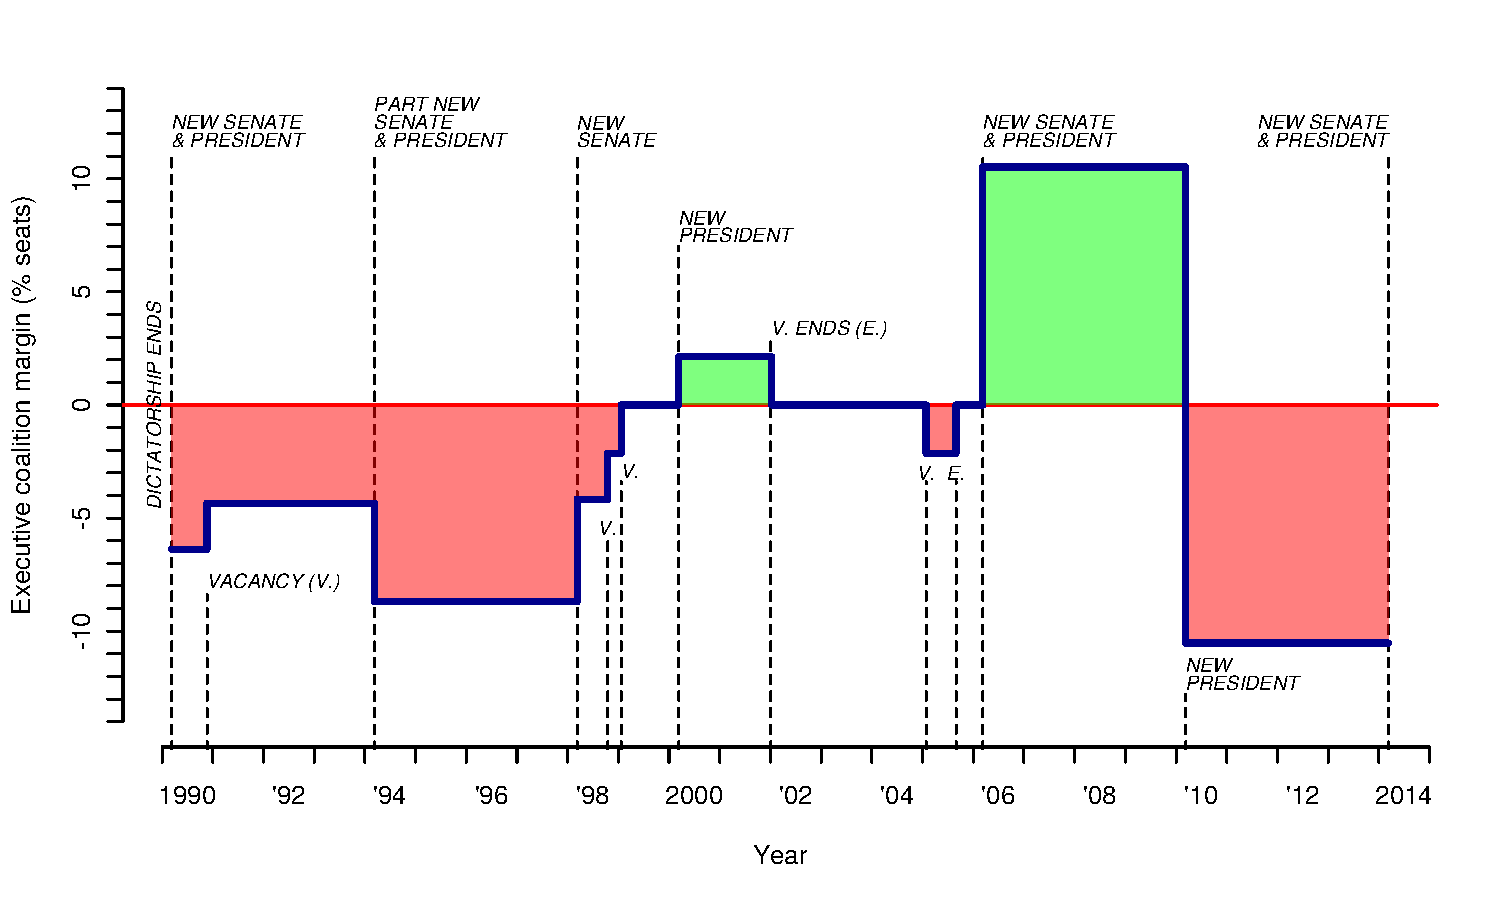
\includegraphics[width=\columnwidth]{../graphs/senChile.pdf}
%% %   \caption{The Conservative chamber. The blue, crenellated line reports, longitudinally, the percentage of Senate seats controlled by the president's coalition minus the percentage controlled by the opposition. Totals include 38 elected senators and, up to 2006, 9 appointed senators and two or less senators for life. Vacancies, if any, are excluded from the denominator (see text). A new Senate is elected every eight years, and was partially renewed in 1994. Vacancies in the period: Ruiz Danyau, Air Force appointee, died in office 11/1990; Pinochet detained in London 10/1998; Errázuriz stripped of immunity 1/1999 (resinstated 1/2002); Lavandero stripped of immunity 1/2005 (replaced upon conviction 8/2005). }\label{f:senChile}
%% % \end{center}
%% % \end{figure}



%% % % \begin{tabular}{lrrrrrr}
%% % %                                   &  \mc{2}{c}{passed}    &  \mc{2}{c}{not}     &  \mc{2}{c}{all}      \\    
%% % % Bills with urgency in             &  N     &  \%          &  N     &  \%        &  N     &  \%         \\ \hline
%% % % $1^{st}$ chamber only              &   122  &  \emph{32}   &   259  &  \emph{68} &   381  &  \emph{100} \\
%% % % $2^{nd}$ chamber only              &   129  &  \emph{68}   &    62  &  \emph{32} &   191  &  \emph{100} \\
%% % % conference only                   &    27  &  \emph{82}   &     6  &  \emph{18} &    33  &  \emph{100} \\
%% % % $1^{st}$ and $2^{nd}$               &   363  &  \emph{81}   &    87  &  \emph{19} &   450  &  \emph{100} \\
%% % % $1^{st}$ and conference            &    39  &  \emph{93}   &     3  &  \emph{7}  &    42  &  \emph{100} \\
%% % % $2^{nd}$ and conference            &    37  &  \emph{90}   &     4  &  \emph{10} &    41  &  \emph{100} \\
%% % % $1^{st}$, $2^{nd}$, and conference  &   212  &  \emph{94}   &    14  &  \emph{6}  &   226  &  \emph{100} \\
%% % % no urgency                        &   541  &  \emph{10}   &  5097  &  \emph{90} &   5638 &  \emph{100} \\ \hline
%% % % %total                             &   929  &  \emph{68}   &   435  &  \emph{32} &  1364  &  \emph{100} \\ \hline
%% % % \end{tabular}

%% % An urgency message can be sent at any stage of the bicameral legislative process, compelling the chamber receiving it to act on a bill. Since urgencies expire once the chamber has finished, it is not uncommon for presidents to send messages at more than one step. Two-fifths of bills with urgencies were deemed so in two or three steps of the legislative process---the first chamber, the second, and/or the bicameral conference.    

%% % % \begin{table}
%% % % \begin{center}
%% % % \begin{tabular}{lrrr|rrr}
%% % %                                   &  \mc{6}{c}{Proposer}                                               \\    
%% % %                                   &  \mc{3}{c}{president}         &  \mc{3}{c}{member of Congress}             \\    
%% % % Bills with urgency in             &  \% pass   & \% not    & ~~~~~N &  \% pass  & \% not    & ~~~~~N \\ \hline
%% % % $1^{st}$ chamber only              &  \emph{40} & \emph{60} & 278  & \emph{12} & \emph{88} & 103  \\
%% % % $2^{nd}$ chamber only              &  \emph{84} & \emph{16} &  98  & \emph{51} & \emph{49} &  93  \\
%% % % conference only                   &  \emph{95} & \emph{5}  &  20  & \emph{62} & \emph{38} &  13  \\
%% % % $1^{st}$ and $2^{nd}$               &  \emph{86} & \emph{14} & 369  & \emph{58} & \emph{42} &  81  \\
%% % % $1^{st}$ and conference            &  \emph{92} & \emph{8}  &  39  & \emph{100}& \emph{0}  &   3  \\
%% % % $2^{nd}$ and conference            &  \emph{100}& \emph{0}  &  18  & \emph{83} & \emph{17} &  23  \\
%% % % $1^{st}$, $2^{nd}$, and conference  &  \emph{94} & \emph{6}  & 192  & \emph{91} & \emph{9}  &  34  \\
%% % % no urgency                        &  \emph{67} & \emph{33} & 455  & \emph{5}  & \emph{95} & 5183  \\ \hline
%% % % \end{tabular}
%% % % \caption{The legislative process, urgency messages, and bill passage by proposer 1998--2014}\label{T:stepsUrgencyPass}
%% % % \end{center}
%% % % \end{table}

%% % \begin{table}
%% % \begin{center}
%% % \begin{tabular}{lrrr|rrr}
%% %                        &  \mc{6}{c}{Proposer}                                               \\    
%% % Step(s) with           &  \mc{3}{c}{president}         &  \mc{3}{c}{member of Congress}             \\    
%% % urgency declared       &  \% pass    & \% not      & ~~~~~N &  \% pass  & \% not      & ~~~~~N \\ \hline
%% % 1 only                 &  \emph{41}  &  \emph{59}  &  285 &  \emph{12}  &  \emph{88}  &  103 \\
%% % 2 only                 &  \emph{84}  &  \emph{16}  &  102 &  \emph{52}  &  \emph{48}  &  96  \\
%% % 3 only                 &  \emph{90}  &  \emph{10}  &  10  &  \emph{75}  &  \emph{25}  &  4   \\
%% % $c$ only               &  \emph{100} &  \emph{0}   &  8   &  \emph{57}  &  \emph{43}  &  7   \\
%% % 1 and 2                &  \emph{85}  &  \emph{15}  &  382 &  \emph{60}  &  \emph{40}  &  84  \\
%% % two of more            &  \emph{100} &  \emph{0}   &  37  &  \emph{90}  &  \emph{10}  &  21  \\
%% % 1, 2, and 3            &  \emph{94}  &  \emph{6}   &  89  &  \emph{90}  &  \emph{10}  &  10  \\
%% % three of more          &  \emph{96}  &  \emph{4}   &  55  &  \emph{86}  &  \emph{14}  &  14  \\
%% % 1, 2, 3, and $c$       &  \emph{93}  &  \emph{7}   &  44  &  \emph{80}  &  \emph{20}  &  10  \\
%% % no urgency             &  \emph{67}  &  \emph{33}  &  457 &  \emph{5}   &  \emph{95}  &  5184 \\ \hline
%% % \end{tabular}
%% % \caption{Legislative steps, urgency messages, and bill passage by proposer 1998--2014. Steps are coded thus: 1 for the chamber of origin, 2 for the revising chamber, 3 for the chamber of origin's response, and $c$ for the conference committee. Cells report bill frequencies.}\label{T:stepsUrgencyPass}
%% % \end{center}
%% % \end{table}







%% % \section{Discussion}

%% % The more difficult it is for an assembly to form and maintain majorities capable of passing legislation, the more attractive it becomes to delegate responsibility to the executive.  Specific examples of situations where decrees may become more attractive are systems where legislative parties have a chronic incapacity to discipline members (as in Brazil), or bicameral systems where malapportionment typically produces majorities of different parties in each house, as in Chile before the removal of appointed senators in 2006 \citep[see][]{carey.shugart.1998a,cox.mccubbins.2001}.

%% % A theme worth pursuing are the determinants of unilateralism.  The logic behind executive vetoes (a concurrent consent institution) extends naturally to executive decrees (a restricted unilateralism institution). In the Linzian framework,\footnote{``[T]here is no democratic principle to resolve [conflict]'' \citeyear[][7]{linz.1994}.} unilateralism appears as unconstitutional moves by the executive to bypass the legislature in the context of impasse---an indicator of deep polarization (also O'Donnell). Presidential unilateralism is tantamount to a democratic system overheating dangerously, perhaps ready to melt into authoritarianism.  The factor driving decree incidence is, again, polarization between the branches. Is there evidence? 

%% % Because it pays attention to a single case giving no constitutional decree authority to its president, Cameron's work remains silent about executive unilateralism.  But following the logic of the bargaining approach, decrees should simply represent one additional tool that the president can resort to in his or her quest for influence on policy.  The veto power has a ``second face'' pointing to silent influence through a capacity of players to anticipate each other's acts; uncertainty reduces that capacity, prompting mistakes and a strategic use of them to gain reputations of toughness in bargaining \citep{cameron.2000,mccarty.1997}.  In the same fashion the decree power hides a second face (e.g. Congress makes a slightly larger concession to the president to avoid a decree of his or hers), and to the extent that players have incomplete information, some should occur and be rescinded as mistakes and reputation-building maneuvers.  

%% % Decrees can also be construed as part of a position-taking game.  It seems plausible that a president decrees some policy knowing, beforehand, that it will be rescinded by the assembly.  The intention is to force the assembly to reject policy popular to his constituents, increase the salience of the issue, and subsequently exploit this when campaigning (or give fellow party members a banner to fly in their campaigns).  Similarly, the assembly may concoct a bill attempting to avoid an executive decree modifying it; in doing so it may miscalculate and make insufficient concessions to the president, prompting the decree which legislators meant to avoid.  



%% \section{Closing remarks}

%% Inspection of urgency message predictors and committee reporting within the time frame that presidential messages set forth has uncovered evidence consistent with consequential urgency authority in Chile. The paper is far from conclusive, however: other than raising an abstract cost of ignoring urgent calls, why members of Congress heed executive cheap talk remains a puzzle. But patterns in the data suggest a promising area for research.  

%% % %% version without urgency step
%% % \begin{sidewaysfigure}
%% % \centering
%% % \begin{tabular}{cc}
%% % %\textbf{Executive-initiated bills} & \textbf{MC-initiated bills} \\
%% % \textbf{Piñera bills sent to Cámara} & \textbf{Piñera bills sent to Senate} \\
%% % ($N=314$) & ($N=90$) \\
%% % \tikzstyle{mid}=[circle,draw]
%% % \tikzstyle{middot}=[circle,draw,dashed]
%% % \begin{tikzpicture}[shorten >=1pt,node distance=2cm,auto,scale=.6]
%% % %\draw[help lines] (-6,-6) grid (6,6);
%% % \node at (-4,6) (st) {\footnotesize{\textbf{\texttt{start}}}};
%% % \node[mid]     at (0,0)   (p)  {\textbf{Exec.}};
%% % \node[mid,green] at (0,6)   (n1) {\textbf{Cám.}};
%% % \node[mid,red]   at (6,0)   (n2) {\textbf{Sen.}};
%% % \node[mid,green] at (0,-6)  (n3) {\textbf{Cám.}};
%% % \node[mid]       at (-6,0)  (c)  {\textbf{Conf.}};
%% % %\node[middot]    at (2,3)   (u)  {$u$};
%% % %\node[middot]    at (3,-2)  (v)  {$u$};
%% % %\node[middot]    at (-2,-3) (w)  {$u$};
%% % %\node[middot]    at (-3,2)  (x)  {$u$};
%% % \draw [-stealth] (st)                    edge node {100} (n1);
%% % \draw [-stealth] (n1) [loop above]       edge node              {22} ();    % l11 $A$
%% % %\draw [-stealth] (n1) [bend left,dashed] edge node              {75} (u);   % l1u $B$
%% % \draw [-stealth] (n1) [out=0,in=90]      edge node              {78} (n2);  % l12 $C$
%% % %\draw [-stealth] (u)  [bend left]        edge node              {14} (n1);  % lu1 $D$
%% % %\draw [-stealth] (u)                     edge node              {61} (n2);  % lu2 $E$
%% % \draw [-stealth] (n2) [loop right]       edge node              {10} ();    % l22 $F$
%% % \draw [-stealth] (n2) [out=-90,in=0]     edge node              {31} (n3);  % l23 $G$
%% % %\draw [-stealth] (n2) [bend left,dashed] edge node              {57} (v);   % l2v $H$
%% % \draw [-stealth] (n2) [out=170, in=10]   edge node [swap]       {36} (p);   % l2p $I$
%% % %\draw [-stealth] (v)  [bend left]        edge node              { 7} (n2);  % lv2 $J$
%% % %\draw [-stealth] (v)                     edge node [swap]       {24} (p)    % lvp $K$
%% % %                 (v)                     edge node              {25} (n3);  % lv3 $L$
%% % \draw [-stealth] (n3) [loop below]       edge node              { 0} ();    % l33 $N$
%% % \draw [-stealth] (n3) [out=180,in=-90]   edge node              { 7} (c);   % l3c $O$
%% % %\draw [-stealth] (n3) [bend left,dashed] edge node              {11} (w);   % l3w $P$
%% % \draw [-stealth] (n3) [out=80, in=-80]   edge node [swap]       {24} (p);   % l3p $Q$
%% % %\draw [-stealth] (w)  [bend left]        edge node [near start] { 0} (n3);  % lw3 $R$
%% % %\draw [-stealth] (w)                     edge node              { 9} (p)    % lwp $S$
%% % %                 (w)                     edge node              { 1} (c);   % lwc $U$
%% % \draw [-stealth] (c)  [loop left]        edge node              { 0} ();    % lcc $V$
%% % %\draw [-stealth] (c)  [bend left,dashed] edge node              { 5} (x);   % lcx $W$
%% % \draw [-stealth] (c)  [out=-10, in=-170] edge node [swap]       { 7} (p);   % lcp $X$
%% % %\draw [-stealth] (x)  [bend left]        edge node              { 0} (c);   % lxc $Y$
%% % %\draw [-stealth] (x)                     edge node              { 5} (p);   % lcp $Z$
%% % \end{tikzpicture}
%% % &
%% % \tikzstyle{mid}=[circle,draw]
%% % \tikzstyle{middot}=[circle,draw,dashed]
%% % \begin{tikzpicture}[shorten >=1pt,node distance=2cm,auto,scale=.6]
%% % %\draw[help lines] (-6,-6) grid (6,6);
%% % \node at (-4,6) (st) {\footnotesize{\textbf{\texttt{start}}}};
%% % \node[mid]       at (0,0)   (p)  {\textbf{Exec.}};
%% % \node[mid,red]   at (0,6)   (n1) {\textbf{Sen.}};
%% % \node[mid,green] at (6,0)   (n2) {\textbf{Cám.}};
%% % \node[mid,red]   at (0,-6)  (n3) {\textbf{Sen.}};
%% % \node[mid]       at (-6,0)  (c)  {\textbf{Conf.}};
%% % %\node[middot]    at (2,3)   (u)  {$u$};
%% % %\node[middot]    at (3,-2)  (v)  {$u$};
%% % %\node[middot]    at (-2,-3) (w)  {$u$};
%% % %\node[middot]    at (-3,2)  (x)  {$u$};
%% % \draw [-stealth] (st)                    edge node {100} (n1);
%% % \draw [-stealth] (n1) [loop above]       edge node              {39} ();    % l11 $A$
%% % %\draw [-stealth] (n1) [bend left,dashed] edge node              {79} (u);   % l1u $B$
%% % \draw [-stealth] (n1) [out=0,in=90]      edge node              {61} (n2);  % l12 $C$
%% % %\draw [-stealth] (u)  [bend left]        edge node              {31} (n1);  % lu1 $D$
%% % %\draw [-stealth] (u)                     edge node              {48} (n2);  % lu2 $E$
%% % \draw [-stealth] (n2) [loop right]       edge node              { 7} ();    % l22 $F$
%% % \draw [-stealth] (n2) [out=-90,in=0]     edge node              {29} (n3);  % l23 $G$
%% % %\draw [-stealth] (n2) [bend left,dashed] edge node              {47} (v);   % l2v $H$
%% % \draw [-stealth] (n2) [out=170, in=10]   edge node [swap]       {26} (p);   % l2p $I$
%% % %\draw [-stealth] (v)  [bend left]        edge node              { 6} (n2);  % lv2 $J$
%% % %\draw [-stealth] (v)                     edge node [swap]       {18} (p)    % lvp $K$
%% % %                 (v)                     edge node              {23} (n3);  % lv3 $L$
%% % \draw [-stealth] (n3) [loop below]       edge node              { 0} ();    % l33 $N$
%% % \draw [-stealth] (n3) [out=180,in=-90]   edge node              {11} (c);   % l3c $O$
%% % %\draw [-stealth] (n3) [bend left,dashed] edge node              {18} (w);   % l3w $P$
%% % \draw [-stealth] (n3) [out=80, in=-80]   edge node [swap]       {18} (p);   % l3p $Q$
%% % %\draw [-stealth] (w)  [bend left]        edge node [near start] { 0} (n3);  % lw3 $R$
%% % %\draw [-stealth] (w)                     edge node              {11} (p)    % lwp $S$
%% % %                 (w)                     edge node              { 7} (c);   % lwc $U$
%% % \draw [-stealth] (c)  [loop left]        edge node              { 2} ();    % lcc $V$
%% % %\draw [-stealth] (c)  [bend left,dashed] edge node              { 8} (x);   % lcx $W$
%% % \draw [-stealth] (c)  [out=-10, in=-170] edge node [swap]       { 9} (p);   % lcp $X$
%% % %\draw [-stealth] (x)  [bend left]        edge node              { 1} (c);   % lxc $Y$
%% % %\draw [-stealth] (x)                     edge node              { 7} (p);   % lcp $Z$
%% % \end{tikzpicture}
%% % \\
%% % \end{tabular}
%% % \caption{Paths of executive bills in Congress. Cám.\, Sen.\, Conf.\, and Exec.\ refer to Cámara de Diputados, Senate, Conference committee, and executive's desk. Numbers are all relative to base 100 (ie., frequency*100/total bills), rounded to nearest integer.}\label{F:billPaths}
%% % \end{sidewaysfigure}

%% %% version with urgency step
%% \begin{sidewaysfigure}%\ContinuedFloat
%% \centering
%% \begin{tabular}{cc}
%% %\textbf{Executive-initiated bills} & \textbf{MC-initiated bills} \\
%% \textbf{Piñera bills sent to Cámara} & \textbf{Piñera bills sent to Senate} \\
%% ($N=314$) & ($N=90$) \\
%% \tikzstyle{mid}=[circle,draw]
%% \tikzstyle{middot}=[circle,draw,dashed]
%% \begin{tikzpicture}[shorten >=1pt,node distance=2cm,auto,scale=.6]
%% %\draw[help lines] (-6,-6) grid (6,6);
%% \node at (-4,6) (st) {\footnotesize{\textbf{\texttt{start}}}};
%% \node[mid]     at (0,0)   (p)  {\textbf{Exec.}};
%% \node[mid,green] at (0,6)   (n1) {\textbf{Cám.}};
%% \node[mid,red]   at (6,0)   (n2) {\textbf{Sen.}};
%% \node[mid,green] at (0,-6)  (n3) {\textbf{Cám.}};
%% \node[mid]       at (-6,0)  (c)  {\textbf{Conf.}};
%% \node[middot]    at (2,3)   (u)  {$u$};
%% \node[middot]    at (3,-2)  (v)  {$u$};
%% \node[middot]    at (-2,-3) (w)  {$u$};
%% \node[middot]    at (-3,2)  (x)  {$u$};
%% \draw [-stealth] (st)                    edge node {100} (n1);
%% \draw [-stealth] (n1) [loop above]       edge node              { 8} ();    % l11 $A$
%% \draw [-stealth] (n1) [bend left,dashed] edge node              {75} (u);   % l1u $B$
%% \draw [-stealth] (n1) [out=0,in=90]      edge node              {17} (n2);  % l12 $C$
%% \draw [-stealth] (u)  [bend left]        edge node              {14} (n1);  % lu1 $D$
%% \draw [-stealth] (u)                     edge node              {61} (n2);  % lu2 $E$
%% \draw [-stealth] (n2) [loop right]       edge node              { 3} ();    % l22 $F$
%% \draw [-stealth] (n2) [out=-90,in=0]     edge node              { 6} (n3);  % l23 $G$
%% \draw [-stealth] (n2) [bend left,dashed] edge node              {57} (v);   % l2v $H$
%% \draw [-stealth] (n2) [out=170, in=10]   edge node [swap]       {12} (p);   % l2p $I$
%% \draw [-stealth] (v)  [bend left]        edge node              { 7} (n2);  % lv2 $J$
%% \draw [-stealth] (v)                     edge node [swap]       {24} (p)    % lvp $K$
%%                  (v)                     edge node              {25} (n3);  % lv3 $L$
%% \draw [-stealth] (n3) [loop below]       edge node              { 0} ();    % l33 $N$
%% \draw [-stealth] (n3) [out=180,in=-90]   edge node              { 6} (c);   % l3c $O$
%% \draw [-stealth] (n3) [bend left,dashed] edge node              {11} (w);   % l3w $P$
%% \draw [-stealth] (n3) [out=80, in=-80]   edge node [swap]       {15} (p);   % l3p $Q$
%% \draw [-stealth] (w)  [bend left]        edge node [near start] { 0} (n3);  % lw3 $R$
%% \draw [-stealth] (w)                     edge node              { 9} (p)    % lwp $S$
%%                  (w)                     edge node              { 1} (c);   % lwc $U$
%% \draw [-stealth] (c)  [loop left]        edge node              { 0} ();    % lcc $V$
%% \draw [-stealth] (c)  [bend left,dashed] edge node              { 5} (x);   % lcx $W$
%% \draw [-stealth] (c)  [out=-10, in=-170] edge node [swap]       { 2} (p);   % lcp $X$
%% \draw [-stealth] (x)  [bend left]        edge node              { 0} (c);   % lxc $Y$
%% \draw [-stealth] (x)                     edge node              { 5} (p);   % lcp $Z$
%% \end{tikzpicture}
%% &
%% \tikzstyle{mid}=[circle,draw]
%% \tikzstyle{middot}=[circle,draw,dashed]
%% \begin{tikzpicture}[shorten >=1pt,node distance=2cm,auto,scale=.6]
%% %\draw[help lines] (-6,-6) grid (6,6);
%% \node at (-4,6) (st) {\footnotesize{\textbf{\texttt{start}}}};
%% \node[mid]       at (0,0)   (p)  {\textbf{Exec.}};
%% \node[mid,red]   at (0,6)   (n1) {\textbf{Sen.}};
%% \node[mid,green] at (6,0)   (n2) {\textbf{Cám.}};
%% \node[mid,red]   at (0,-6)  (n3) {\textbf{Sen.}};
%% \node[mid]       at (-6,0)  (c)  {\textbf{Conf.}};
%% \node[middot]    at (2,3)   (u)  {$u$};
%% \node[middot]    at (3,-2)  (v)  {$u$};
%% \node[middot]    at (-2,-3) (w)  {$u$};
%% \node[middot]    at (-3,2)  (x)  {$u$};
%% \draw [-stealth] (st)                    edge node {100} (n1);
%% \draw [-stealth] (n1) [loop above]       edge node              { 8} ();    % l11 $A$
%% \draw [-stealth] (n1) [bend left,dashed] edge node              {79} (u);   % l1u $B$
%% \draw [-stealth] (n1) [out=0,in=90]      edge node              {13} (n2);  % l12 $C$
%% \draw [-stealth] (u)  [bend left]        edge node              {31} (n1);  % lu1 $D$
%% \draw [-stealth] (u)                     edge node              {48} (n2);  % lu2 $E$
%% \draw [-stealth] (n2) [loop right]       edge node              { 1} ();    % l22 $F$
%% \draw [-stealth] (n2) [out=-90,in=0]     edge node              { 6} (n3);  % l23 $G$
%% \draw [-stealth] (n2) [bend left,dashed] edge node              {47} (v);   % l2v $H$
%% \draw [-stealth] (n2) [out=170, in=10]   edge node [swap]       { 8} (p);   % l2p $I$
%% \draw [-stealth] (v)  [bend left]        edge node              { 6} (n2);  % lv2 $J$
%% \draw [-stealth] (v)                     edge node [swap]       {18} (p)    % lvp $K$
%%                  (v)                     edge node              {23} (n3);  % lv3 $L$
%% \draw [-stealth] (n3) [loop below]       edge node              { 0} ();    % l33 $N$
%% \draw [-stealth] (n3) [out=180,in=-90]   edge node              { 4} (c);   % l3c $O$
%% \draw [-stealth] (n3) [bend left,dashed] edge node              {18} (w);   % l3w $P$
%% \draw [-stealth] (n3) [out=80, in=-80]   edge node [swap]       { 7} (p);   % l3p $Q$
%% \draw [-stealth] (w)  [bend left]        edge node [near start] { 0} (n3);  % lw3 $R$
%% \draw [-stealth] (w)                     edge node              {11} (p)    % lwp $S$
%%                  (w)                     edge node              { 7} (c);   % lwc $U$
%% \draw [-stealth] (c)  [loop left]        edge node              { 1} ();    % lcc $V$
%% \draw [-stealth] (c)  [bend left,dashed] edge node              { 8} (x);   % lcx $W$
%% \draw [-stealth] (c)  [out=-10, in=-170] edge node [swap]       { 2} (p);   % lcp $X$
%% \draw [-stealth] (x)  [bend left]        edge node              { 1} (c);   % lxc $Y$
%% \draw [-stealth] (x)                     edge node              { 7} (p);   % lcp $Z$
%% \end{tikzpicture}
%% \\
%% \end{tabular}
%% %\caption{Paths of executive bills (cont.\ distinguishing urgencies)}
%% \caption{Paths of executive bills in Congress 2010--14. Cám.\, Sen.\, Conf.\, and Exec.\ refer to Cámara de Diputados, Senate, Conference committee, and executive's desk, respectively. Numbers are all relative to base 100 (i.e., freq.$\times$100/\emph{N}), rounded to nearest integer.}\label{F:billPaths}
%% \end{sidewaysfigure}

%% The big challenge is a method to deal with the selection problem complicating analysis of the urgency--bill passage relation. I close with a look at the bigger picture to give an idea of this obstacle. Figure \ref{F:billPaths} follows President Piñera's proposals ($N=394$) along the full bicameral legislative process, keeping Cámara- (left panel) and Senate-initiated bills (right) separate. The diagram reports relative numbers of proposals in the different paths (atop arrows), distinguishing proposals that proceeded to the next node (i.e., bills that passed, possibly amended) from those that did not (bills rejected, pending, or never considered). It also separates bills that became urgent (the dashed paths) from those that did not. Plots show that urgencies cannot always overcome obstacles in the process. Piñera faced an opposition-controlled Senate throughout his term, yet declared similar proportions of Cámara- and Senate-initiated bills urgent (75 and 79 percent, respectively). The key difference is related to presidential anticipation of rougher terrain in the upper chamber, Piñera sending four out of five proposals to the Cámara. Those he did sent to the Senate were, in fact, less likely to proceed to the next node than the Cámara-initiated ($17+61=78$ v\ $13+48=61$ percent). Also noteworthy is that half as many urgencies in the Cámara failed to move the bill forward compared to the Senate  (14 v 31 percent). If urgency messages trigger reports to the Congressional floor in predictable ways, they are certainly no guarantee of executive success: two out of five urgent Senate-initiated bills ($31/79$) never reached the revising stage, and one-fith in the lower chamber ($14/75$). Few chamber of origin differences arised once legislation reached the second node (relative to the traffic arriving there). Only the shares of bills amended in revising chamber, and therefore sent back to the originating, are somewhat different ($(25+6)/78=.4$ for Cámara-initiated bills, $(23+6)/61=.48$ for Senate-initiated bills). Differences arise again in the third node (when the originating chamber can either concur with amendments by the revising or proceed to conference). Interestingly, the share of urgent bills in third node not proceeding further collapses to zero, regardless of chamber of origin. But the proportion of urgent Senate-initiated bills ($18/(23+6)=.62$) was substantially higher than the Cámara-initiated ($11/(25+6)=.35$). Urgency and success are more strongly associated at later stages of the legislative process. 

%% The urgency authority in the continent is an institution worth studying more carefully. The next chapter inspects it in Brazil, where it is related to executive unilaterlism. Unlike Chile's, the Brazilian reversionary outcome and agenda play in favor of executive influence, simplifying analysis considerably.

%% %To stimulate debate, I close with a bigger picture of the urgency--bill passage relation. Figure \ref{F:billPaths} follows 394 proposals by President Piñera along the bicameral legislative process. Facing an opposition-controlled Senate throughout his term, Piñera chose to send four out of five bills to the Cámara. The diagram reports relative numbers of proposals in the different paths (atop arrows), distinguishing proposals that proceeded to the next chamber (i.e., bills that passed, possibly amended) from those that did not (bills rejected, pending, or never considered). It also separates bills that became urgent (the dashed paths) from those that did not. Initial differences across chambers are notable: if shares of bills tagged urgent in the Cámara and Senate are very similar (75 and 79 percent, respectively), nearly one-fifth more proceeded to the next node in the former than the latter ($17+61=78$ vs.\ $13+48=61$ percent). The failure differential may explain the executive's preference for lower-chamber initiation, but not why Piñera still chose to initiate 90 bills in the Senate. Also noteworthy is that half as many urgencies in the Cámara failed to move the bill forward compared to the Senate  (14 and 31 percent, respectively). If, as seen in the chapter, urgency messages trigger movement in Congress in predictable ways, they are certainly no guarantee of executive success: two out of five urgent bills in the Senate ($31/79$) never reached the Cámara, one-fith in the lower chamber ($14/75$) did not make it to the Senate. Moving to the next node in the legislative process reveals that most inter-chamber differences vanish in the revising chamber: proportions of bills passed unamended by the second chamber and therefore sent to the executive's desk are similar ($(12+24=36)/78=.46$ for Cámara-initiated proposals and $(8+18=26)/61=.43$ for the Senate-initiated), as are shares of proposals declared urgent ($57/78=.73$ and $47/61=.77$, respectively) and shares of urgencies failing to push the bill forward ($7/57=.12$ and $6/47=.13$, respectively). Only the shares of bills amended in second chamber and therefore sent back to the originating chamber change slightly ($(25+6)/78=.4$ for Cámara-initiated bills, $(23+6)/61=.48$ for Senate-initiated bills). And differences reappear further down, the originating chamber concurring with amendments more often in Cámara- than in Senate-initiated bills (.77 v .62), less bills calling for urgency (.35 v .62), and fewer going to conference. While the urgency authority is certainly related to success, it is hardly determinant. 


%% % \section{Online appendix}
%% %
%% % Bill urgency logit models. 
%% %
%% % \begin{verbatim}
%% % > summary(fit1)
%% %
%% % Call:
%% % glm(formula = dv ~ dmocion + drefHda + dmajSen + dinSen + ptermR + 
%% %     legyrR + dreform2010, family = binomial(link = logit), data = tmpdat)
%% %
%% % Deviance Residuals: 
%% %     Min       1Q   Median       3Q      Max  
%% % -2.2416  -0.3734  -0.3311  -0.2942   2.5993  
%% %
%% % Coefficients:
%% %             Estimate Std. Error z value Pr(>|z|)    
%% % (Intercept)  0.11684    0.16082   0.727   0.4675    
%% % dmocion     -2.98974    0.09096 -32.868   <2e-16 ***
%% % drefHda      1.76145    0.11077  15.902   <2e-16 ***
%% % dmajSen     -0.12186    0.15900  -0.766   0.4434    
%% % dinSen       0.18243    0.09609   1.898   0.0576 .  
%% % ptermR       0.10363    0.04195   2.470   0.0135 *  
%% % legyrR       0.07784    0.04228   1.841   0.0656 .  
%% % dreform2010  0.22938    0.16788   1.366   0.1718    
%% % ---
%% % Signif. codes:  0 ‘***’ 0.001 ‘**’ 0.01 ‘*’ 0.05 ‘.’ 0.1 ‘ ’ 1
%% %
%% % (Dispersion parameter for binomial family taken to be 1)
%% %
%% %     Null deviance: 6893.3  on 6986  degrees of freedom
%% % Residual deviance: 4111.3  on 6979  degrees of freedom
%% % AIC: 4127.3
%% %
%% % Number of Fisher Scoring iterations: 5
%% %
%% % > summary(fit2)
%% %
%% % Call:
%% % glm(formula = dv ~ dmocionAllOpp + dmocionMix + dmocionAllPdt + 
%% %     drefHda + dmajSen + dinSen + ptermR + legyrR + dreform2010, 
%% %     family = binomial(link = logit), data = tmpdat)
%% %
%% % Deviance Residuals: 
%% %     Min       1Q   Median       3Q      Max  
%% % -2.3227  -0.3973  -0.3235  -0.2243   2.7781  
%% %
%% % Coefficients:
%% %               Estimate Std. Error z value Pr(>|z|)    
%% % (Intercept)    0.11287    0.16244   0.695 0.487163    
%% % dmocionAllOpp -3.60272    0.13728 -26.244  < 2e-16 ***
%% % dmocionMix    -2.53044    0.11534 -21.939  < 2e-16 ***
%% % dmocionAllPdt -2.97420    0.12626 -23.557  < 2e-16 ***
%% % drefHda        1.78289    0.11134  16.014  < 2e-16 ***
%% % dmajSen       -0.16221    0.16069  -1.009 0.312758    
%% % dinSen         0.41216    0.11095   3.715 0.000203 ***
%% % ptermR         0.11042    0.04231   2.610 0.009066 ** 
%% % legyrR         0.08018    0.04246   1.888 0.058985 .  
%% % dreform2010    0.17586    0.16987   1.035 0.300545    
%% % ---
%% % Signif. codes:  0 ‘***’ 0.001 ‘**’ 0.01 ‘*’ 0.05 ‘.’ 0.1 ‘ ’ 1
%% %
%% % (Dispersion parameter for binomial family taken to be 1)
%% %
%% %     Null deviance: 6893.3  on 6986  degrees of freedom
%% % Residual deviance: 4057.5  on 6977  degrees of freedom
%% % AIC: 4077.5
%% %
%% % Number of Fisher Scoring iterations: 6
%% %
%% % > summary(fit3)
%% %
%% % Call:
%% % glm(formula = dv ~ dmocionAllOpp + dmocionMix + dmocionAllPdt + 
%% %     drefHda + dmajSen + dinSen + ptermR + legyrR + dreform2010 + 
%% %     as.factor(legis), family = binomial(link = logit), data = tmpdat)
%% %
%% % Deviance Residuals: 
%% %     Min       1Q   Median       3Q      Max  
%% % -2.3350  -0.4107  -0.3142  -0.2291   2.9115  
%% %
%% % Coefficients:
%% %                      Estimate Std. Error z value Pr(>|z|)    
%% % (Intercept)           0.26152    0.21057   1.242  0.21425    
%% % dmocionAllOpp        -3.70649    0.14072 -26.339  < 2e-16 ***
%% % dmocionMix           -2.64589    0.11967 -22.109  < 2e-16 ***
%% % dmocionAllPdt        -3.07657    0.13046 -23.582  < 2e-16 ***
%% % drefHda               1.75917    0.11215  15.686  < 2e-16 ***
%% % dmajSen              -0.37065    0.20868  -1.776  0.07570 .  
%% % dinSen                0.39545    0.11149   3.547  0.00039 ***
%% % ptermR                0.08349    0.04646   1.797  0.07235 .  
%% % legyrR                0.08452    0.04279   1.975  0.04825 *  
%% % dreform2010           0.17376    0.28896   0.601  0.54764    
%% % as.factor(legis)2002 -0.23155    0.15496  -1.494  0.13512    
%% % as.factor(legis)2006  0.33323    0.14608   2.281  0.02254 *  
%% % as.factor(legis)2010 -0.06295    0.35112  -0.179  0.85771    
%% % ---
%% % Signif. codes:  0 ‘***’ 0.001 ‘**’ 0.01 ‘*’ 0.05 ‘.’ 0.1 ‘ ’ 1
%% %
%% % (Dispersion parameter for binomial family taken to be 1)
%% %
%% %     Null deviance: 6893.3  on 6986  degrees of freedom
%% % Residual deviance: 4037.8  on 6974  degrees of freedom
%% % AIC: 4063.8
%% %
%% % Number of Fisher Scoring iterations: 6
%% %
%% % > summary(fit4)
%% % Generalized linear mixed model fit by maximum likelihood (Laplace Approximation) ['glmerMod']
%% %  Family: binomial  ( logit )
%% % Formula: dv ~ dmocionAllOpp + dmocionMix + dmocionAllPdt + drefHda + dmajSen +      dinSen + ptermR + legyrR + dreform2010 + (1 | legis)
%% %    Data: tmpdat
%% %
%% %      AIC      BIC   logLik deviance df.resid 
%% %   4070.5   4145.9  -2024.3   4048.5     6976 
%% %
%% % Scaled residuals: 
%% %     Min      1Q  Median      3Q     Max 
%% % -3.7614 -0.2940 -0.2263 -0.1634  7.9304 
%% %
%% % Random effects:
%% %  Groups Name        Variance Std.Dev.
%% %  legis  (Intercept) 0.03167  0.1779  
%% % Number of obs: 6987, groups:  legis, 4
%% %
%% % Fixed effects:
%% %               Estimate Std. Error z value Pr(>|z|)    
%% % (Intercept)    0.23385    0.19175   1.220 0.222616    
%% % dmocionAllOpp -3.68591    0.14074 -26.190  < 2e-16 ***
%% % dmocionMix    -2.62186    0.11990 -21.868  < 2e-16 ***
%% % dmocionAllPdt -3.05558    0.13038 -23.436  < 2e-16 ***
%% % drefHda        1.76379    0.11203  15.743  < 2e-16 ***
%% % dmajSen       -0.30920    0.18177  -1.701 0.088925 .  
%% % dinSen         0.39843    0.11135   3.578 0.000346 ***
%% % ptermR         0.08657    0.04425   1.956 0.050428 .  
%% % legyrR         0.08324    0.04269   1.950 0.051202 .  
%% % dreform2010    0.13795    0.20817   0.663 0.507523    
%% % ---
%% % Signif. codes:  0 ‘***’ 0.001 ‘**’ 0.01 ‘*’ 0.05 ‘.’ 0.1 ‘ ’ 1
%% %
%% % Correlation of Fixed Effects:
%% %             (Intr) dmcnAO dmcnMx dmcnAP drefHd dmajSn dinSen ptermR legyrR
%% % dmocnAllOpp -0.204                                                        
%% % dmocionMix  -0.255  0.324                                                 
%% % dmocnAllPdt -0.193  0.399  0.320                                          
%% % drefHda     -0.211  0.167  0.250  0.189                                   
%% % dmajSen     -0.766  0.076  0.056  0.058  0.026                            
%% % dinSen      -0.114 -0.223  0.184 -0.336  0.065  0.009                     
%% % ptermR       0.104 -0.093 -0.080 -0.055  0.040 -0.117 -0.018              
%% % legyrR      -0.130 -0.038 -0.043 -0.014  0.042  0.147  0.011 -0.146       
%% % dreform2010 -0.535 -0.021 -0.084 -0.028  0.008  0.454 -0.007  0.043  0.146
%% % > display(fit4)            
%% % glmer(formula = dv ~ dmocionAllOpp + dmocionMix + dmocionAllPdt + 
%% %     drefHda + dmajSen + dinSen + ptermR + legyrR + dreform2010 + 
%% %     (1 | legis), data = tmpdat, family = binomial(link = "logit"))
%% %               coef.est coef.se
%% % (Intercept)    0.23     0.19  
%% % dmocionAllOpp -3.69     0.14  
%% % dmocionMix    -2.62     0.12  
%% % dmocionAllPdt -3.06     0.13  
%% % drefHda        1.76     0.11  
%% % dmajSen       -0.31     0.18  
%% % dinSen         0.40     0.11  
%% % ptermR         0.09     0.04  
%% % legyrR         0.08     0.04  
%% % dreform2010    0.14     0.21  
%% %
%% % Error terms:
%% %  Groups   Name        Std.Dev.
%% %  legis    (Intercept) 0.18    
%% %  Residual             1.00    
%% % ---
%% % number of obs: 6987, groups: legis, 4
%% % AIC = 4070.5, DIC = 4028.8
%% % deviance = 4038.6 
%% % \end{verbatim}
%% %
%% % Report before deadline logit models
%% %
%% % \begin{verbatim}
%% % > summary(fit1)
%% %
%% % Call:
%% % glm(formula = dhdaReportwiDeadline ~ d2wk + d4wk + dextend + 
%% %     dwithdr + dmocion + dmajSen + dsen + ptermR + legyrR + dreform2010, 
%% %     family = binomial(link = logit), data = chainsHda)
%% %
%% % Deviance Residuals: 
%% %     Min       1Q   Median       3Q      Max  
%% % -2.9603   0.3297   0.5408   0.7358   1.2914  
%% %
%% % Coefficients:
%% %             Estimate Std. Error z value Pr(>|z|)    
%% % (Intercept)  1.18006    0.29436   4.009 6.10e-05 ***
%% % d2wk         0.28504    0.14527   1.962  0.04976 *  
%% % d4wk        -0.12495    0.14943  -0.836  0.40304    
%% % dextend      0.53540    0.12442   4.303 1.68e-05 ***
%% % dwithdr      0.32239    0.12224   2.637  0.00836 ** 
%% % dmocion      1.71152    0.28648   5.974 2.31e-09 ***
%% % dmajSen     -0.30532    0.28433  -1.074  0.28290    
%% % dsen         0.24700    0.12046   2.050  0.04033 *  
%% % ptermR       0.40829    0.05523   7.393 1.44e-13 ***
%% % legyrR       0.10092    0.05148   1.960  0.04998 *  
%% % dreform2010 -0.60279    0.28528  -2.113  0.03460 *  
%% % ---
%% % Signif. codes:  0 ‘***’ 0.001 ‘**’ 0.01 ‘*’ 0.05 ‘.’ 0.1 ‘ ’ 1
%% %
%% % (Dispersion parameter for binomial family taken to be 1)
%% %
%% %     Null deviance: 2802.2  on 2684  degrees of freedom
%% % Residual deviance: 2572.3  on 2674  degrees of freedom
%% % AIC: 2594.3
%% %
%% % Number of Fisher Scoring iterations: 5
%% %
%% % > summary(fit2)
%% %
%% % Call:
%% % glm(formula = dhdaReportwiDeadline ~ d2wk + d4wk + dextend + 
%% %     dwithdr + dmocionAllPdt + dmocionMix + dmocionAllOpp + dmajSen + 
%% %     dsen + ptermR + legyrR + dreform2010, family = binomial(link = logit), 
%% %     data = chainsHda)
%% %
%% % Deviance Residuals: 
%% %     Min       1Q   Median       3Q      Max  
%% % -3.2376   0.2876   0.5416   0.7363   1.2959  
%% %
%% % Coefficients:
%% %               Estimate Std. Error z value Pr(>|z|)    
%% % (Intercept)    1.18549    0.29417   4.030 5.58e-05 ***
%% % d2wk           0.26735    0.14541   1.839  0.06598 .  
%% % d4wk          -0.12476    0.14940  -0.835  0.40367    
%% % dextend        0.54032    0.12403   4.356 1.32e-05 ***
%% % dwithdr        0.33205    0.12209   2.720  0.00653 ** 
%% % dmocionAllPdt  0.51282    0.50969   1.006  0.31435    
%% % dmocionMix     0.39343    0.54712   0.719  0.47208    
%% % dmocionAllOpp  2.57030    0.46204   5.563 2.65e-08 ***
%% % dmajSen       -0.30107    0.28417  -1.059  0.28939    
%% % dsen           0.25873    0.12031   2.151  0.03151 *  
%% % ptermR         0.41115    0.05529   7.437 1.03e-13 ***
%% % legyrR         0.09957    0.05157   1.931  0.05352 .  
%% % dreform2010   -0.61593    0.28503  -2.161  0.03070 *  
%% % ---
%% % Signif. codes:  0 ‘***’ 0.001 ‘**’ 0.01 ‘*’ 0.05 ‘.’ 0.1 ‘ ’ 1
%% %
%% % (Dispersion parameter for binomial family taken to be 1)
%% %
%% %     Null deviance: 2802.2  on 2684  degrees of freedom
%% % Residual deviance: 2559.1  on 2672  degrees of freedom
%% % AIC: 2585.1
%% %
%% % Number of Fisher Scoring iterations: 5
%% %
%% % > summary(fit3)
%% %
%% % Call:
%% % glm(formula = dhdaReportwiDeadline ~ d2wk + d4wk + dextend + 
%% %     dwithdr + dmocionAllPdt + dmocionMix + dmocionAllOpp + dmajSen + 
%% %     dsen + ptermR + legyrR + dreform2010 + as.factor(legis), 
%% %     family = binomial(link = logit), data = chainsHda)
%% %
%% % Deviance Residuals: 
%% %     Min       1Q   Median       3Q      Max  
%% % -3.1773   0.2884   0.5244   0.7354   1.3038  
%% %
%% % Coefficients:
%% %                      Estimate Std. Error z value Pr(>|z|)    
%% % (Intercept)           1.17183    0.34950   3.353 0.000800 ***
%% % d2wk                  0.25220    0.14658   1.721 0.085333 .  
%% % d4wk                 -0.15061    0.15071  -0.999 0.317635    
%% % dextend               0.58774    0.12665   4.641 3.47e-06 ***
%% % dwithdr               0.43067    0.12695   3.392 0.000693 ***
%% % dmocionAllPdt         0.46282    0.51408   0.900 0.367971    
%% % dmocionMix            0.55614    0.54884   1.013 0.310913    
%% % dmocionAllOpp         2.60046    0.46212   5.627 1.83e-08 ***
%% % dmajSen              -0.07306    0.32717  -0.223 0.823305    
%% % dsen                  0.24309    0.12127   2.005 0.045014 *  
%% % ptermR                0.42149    0.05715   7.375 1.65e-13 ***
%% % legyrR                0.09587    0.05174   1.853 0.063857 .  
%% % dreform2010          -0.41916    0.62553  -0.670 0.502794    
%% % as.factor(legis)2002  0.03543    0.21769   0.163 0.870704    
%% % as.factor(legis)2006 -0.57643    0.21256  -2.712 0.006692 ** 
%% % as.factor(legis)2010 -0.19056    0.70618  -0.270 0.787282    
%% % ---
%% % Signif. codes:  0 ‘***’ 0.001 ‘**’ 0.01 ‘*’ 0.05 ‘.’ 0.1 ‘ ’ 1
%% %
%% % (Dispersion parameter for binomial family taken to be 1)
%% %
%% %     Null deviance: 2802.2  on 2684  degrees of freedom
%% % Residual deviance: 2544.4  on 2669  degrees of freedom
%% % AIC: 2576.4
%% %
%% % Number of Fisher Scoring iterations: 5
%% %
%% % > summary(fit4)
%% % Generalized linear mixed model fit by maximum likelihood (Laplace Approximation) ['glmerMod']
%% %  Family: binomial  ( logit )
%% % Formula: dhdaReportwiDeadline ~ d2wk + d4wk + dextend + dwithdr + dmocionAllPdt +  
%% %     dmocionMix + dmocionAllOpp + dmajSen + dsen + ptermR + legyrR +      dreform2010 + (1 | legis)
%% %    Data: chainsHda
%% %
%% %      AIC      BIC   logLik deviance df.resid 
%% %   2582.6   2665.1  -1277.3   2554.6     2671 
%% %
%% % Scaled residuals: 
%% %      Min       1Q   Median       3Q      Max 
%% % -12.7678   0.2061   0.3861   0.5626   1.1551 
%% %
%% % Random effects:
%% %  Groups Name        Variance Std.Dev.
%% %  legis  (Intercept) 0.04002  0.2001  
%% % Number of obs: 2685, groups:  legis, 4
%% %
%% % Fixed effects:
%% %               Estimate Std. Error z value Pr(>|z|)    
%% % (Intercept)    1.04712    0.31578   3.316 0.000913 ***
%% % d2wk           0.25832    0.14616   1.767 0.077167 .  
%% % d4wk          -0.14152    0.15032  -0.941 0.346499    
%% % dextend        0.57378    0.12614   4.549 5.40e-06 ***
%% % dwithdr        0.40208    0.12706   3.164 0.001554 ** 
%% % dmocionAllPdt  0.47523    0.51265   0.927 0.353924    
%% % dmocionMix     0.51133    0.54916   0.931 0.351801    
%% % dmocionAllOpp  2.59277    0.46236   5.608 2.05e-08 ***
%% % dmajSen       -0.14504    0.29674  -0.489 0.624997    
%% % dsen           0.24673    0.12092   2.040 0.041310 *  
%% % ptermR         0.41907    0.05563   7.534 4.94e-14 ***
%% % legyrR         0.09640    0.05164   1.867 0.061946 .  
%% % dreform2010   -0.47834    0.33971  -1.408 0.159109    
%% % ---
%% % Signif. codes:  0 ‘***’ 0.001 ‘**’ 0.01 ‘*’ 0.05 ‘.’ 0.1 ‘ ’ 1
%% %
%% % Correlation of Fixed Effects:
%% %             (Intr) d2wk   d4wk   dextnd dwthdr dmcnAP dmcnMx dmcnAO dmajSn dsen   ptermR legyrR
%% % d2wk        -0.236                                                                             
%% % d4wk        -0.251  0.706                                                                      
%% % dextend     -0.080 -0.102 -0.124                                                               
%% % dwithdr     -0.115 -0.053 -0.053 -0.351                                                        
%% % dmocnAllPdt  0.004  0.004 -0.033 -0.008 -0.012                                                 
%% % dmocionMix  -0.014  0.000 -0.021  0.021 -0.007  0.006                                          
%% % dmocnAllOpp  0.002 -0.041 -0.030  0.022  0.016  0.009  0.007                                   
%% % dmajSen     -0.805 -0.068 -0.072  0.020  0.028 -0.007  0.007  0.001                            
%% % dsen        -0.106  0.041  0.039 -0.261  0.040 -0.035 -0.007  0.012 -0.021                     
%% % ptermR       0.088  0.017 -0.110 -0.008 -0.007  0.063 -0.046  0.031 -0.057 -0.041              
%% % legyrR      -0.078 -0.097 -0.035  0.098  0.027  0.011  0.004  0.001  0.101 -0.003 -0.138       
%% % dreform2010 -0.739 -0.104 -0.061  0.066  0.087 -0.005  0.000 -0.017  0.698  0.052  0.017  0.092
%% % > display(fit4)
%% % glmer(formula = dhdaReportwiDeadline ~ d2wk + d4wk + dextend + 
%% %     dwithdr + dmocionAllPdt + dmocionMix + dmocionAllOpp + dmajSen + 
%% %     dsen + ptermR + legyrR + dreform2010 + (1 | legis), data = chainsHda, 
%% %     family = binomial(link = "logit"))
%% %               coef.est coef.se
%% % (Intercept)    1.05     0.32  
%% % d2wk           0.26     0.15  
%% % d4wk          -0.14     0.15  
%% % dextend        0.57     0.13  
%% % dwithdr        0.40     0.13  
%% % dmocionAllPdt  0.48     0.51  
%% % dmocionMix     0.51     0.55  
%% % dmocionAllOpp  2.59     0.46  
%% % dmajSen       -0.15     0.30  
%% % dsen           0.25     0.12  
%% % ptermR         0.42     0.06  
%% % legyrR         0.10     0.05  
%% % dreform2010   -0.48     0.34  
%% %
%% % Error terms:
%% %  Groups   Name        Std.Dev.
%% %  legis    (Intercept) 0.20    
%% %  Residual             1.00    
%% % ---
%% % number of obs: 2685, groups: legis, 4
%% % AIC = 2582.6, DIC = 2536.7
%% % deviance = 2545.6 
%% % > summary(fit11)
%% %
%% % Call:
%% % glm(formula = danyReportwiDeadline ~ d2wk + d4wk + dextend + 
%% %     dwithdr + dmocion + dmajSen + dsen + ptermR + legyrR + dreform2010, 
%% %     family = binomial(link = logit), data = chainsAll)
%% %
%% % Deviance Residuals: 
%% %     Min       1Q   Median       3Q      Max  
%% % -2.5015   0.3943   0.5290   0.6614   1.2312  
%% %
%% % Coefficients:
%% %               Estimate Std. Error z value Pr(>|z|)    
%% % (Intercept)  1.2066052  0.2290612   5.268 1.38e-07 ***
%% % d2wk         0.7467455  0.1255854   5.946 2.75e-09 ***
%% % d4wk         0.0176985  0.1210476   0.146 0.883755    
%% % dextend      0.3590112  0.1025663   3.500 0.000465 ***
%% % dwithdr      0.0355593  0.0987402   0.360 0.718750    
%% % dmocion     -0.6354063  0.0915810  -6.938 3.97e-12 ***
%% % dmajSen     -0.1357915  0.2146847  -0.633 0.527050    
%% % dsen         0.2728576  0.0914901   2.982 0.002860 ** 
%% % ptermR       0.3186034  0.0432412   7.368 1.73e-13 ***
%% % legyrR       0.0622340  0.0413198   1.506 0.132027    
%% % dreform2010  0.0009288  0.2186480   0.004 0.996611    
%% % ---
%% % Signif. codes:  0 ‘***’ 0.001 ‘**’ 0.01 ‘*’ 0.05 ‘.’ 0.1 ‘ ’ 1
%% %
%% % (Dispersion parameter for binomial family taken to be 1)
%% %
%% %     Null deviance: 4258.3  on 4627  degrees of freedom
%% % Residual deviance: 4048.9  on 4617  degrees of freedom
%% % AIC: 4070.9
%% %
%% % Number of Fisher Scoring iterations: 4
%% %
%% % > summary(fit12)
%% %
%% % Call:
%% % glm(formula = danyReportwiDeadline ~ d2wk + d4wk + dextend + 
%% %     dwithdr + dmocionAllPdt + dmocionMix + dmocionAllOpp + dmajSen + 
%% %     dsen + ptermR + legyrR + dreform2010, family = binomial(link = logit), 
%% %     data = chainsAll)
%% %
%% % Deviance Residuals: 
%% %     Min       1Q   Median       3Q      Max  
%% % -2.5196   0.3857   0.5212   0.6490   1.3508  
%% %
%% % Coefficients:
%% %               Estimate Std. Error z value Pr(>|z|)    
%% % (Intercept)    1.21973    0.23008   5.301 1.15e-07 ***
%% % d2wk           0.72669    0.12617   5.760 8.43e-09 ***
%% % d4wk           0.01802    0.12175   0.148 0.882304    
%% % dextend        0.35836    0.10290   3.483 0.000496 ***
%% % dwithdr        0.06819    0.09932   0.687 0.492356    
%% % dmocionAllPdt -0.98924    0.14252  -6.941 3.90e-12 ***
%% % dmocionMix    -0.84932    0.12885  -6.592 4.35e-11 ***
%% % dmocionAllOpp  0.13265    0.17941   0.739 0.459676    
%% % dmajSen       -0.12345    0.21574  -0.572 0.567179    
%% % dsen           0.28175    0.09190   3.066 0.002170 ** 
%% % ptermR         0.32950    0.04344   7.585 3.32e-14 ***
%% % legyrR         0.06238    0.04153   1.502 0.133134    
%% % dreform2010   -0.05703    0.21961  -0.260 0.795112    
%% % ---
%% % Signif. codes:  0 ‘***’ 0.001 ‘**’ 0.01 ‘*’ 0.05 ‘.’ 0.1 ‘ ’ 1
%% %
%% % (Dispersion parameter for binomial family taken to be 1)
%% %
%% %     Null deviance: 4258.3  on 4627  degrees of freedom
%% % Residual deviance: 4016.5  on 4615  degrees of freedom
%% % AIC: 4042.5
%% %
%% % Number of Fisher Scoring iterations: 4
%% %
%% % > summary(fit13)
%% %
%% % Call:
%% % glm(formula = danyReportwiDeadline ~ d2wk + d4wk + dextend + 
%% %     dwithdr + dmocionAllPdt + dmocionMix + dmocionAllOpp + dmajSen + 
%% %     dsen + ptermR + legyrR + dreform2010 + as.factor(legis), 
%% %     family = binomial(link = logit), data = chainsAll)
%% %
%% % Deviance Residuals: 
%% %     Min       1Q   Median       3Q      Max  
%% % -2.5109   0.3843   0.5211   0.6490   1.3289  
%% %
%% % Coefficients:
%% %                      Estimate Std. Error z value Pr(>|z|)    
%% % (Intercept)           1.19142    0.27736   4.296 1.74e-05 ***
%% % d2wk                  0.72576    0.12631   5.746 9.15e-09 ***
%% % d4wk                  0.01370    0.12183   0.112 0.910468    
%% % dextend               0.37244    0.10415   3.576 0.000349 ***
%% % dwithdr               0.10387    0.10199   1.018 0.308448    
%% % dmocionAllPdt        -0.97782    0.14297  -6.839 7.97e-12 ***
%% % dmocionMix           -0.82984    0.12934  -6.416 1.40e-10 ***
%% % dmocionAllOpp         0.14936    0.17968   0.831 0.405843    
%% % dmajSen              -0.05406    0.25238  -0.214 0.830381    
%% % dsen                  0.27508    0.09213   2.986 0.002830 ** 
%% % ptermR                0.33252    0.04550   7.309 2.69e-13 ***
%% % legyrR                0.06045    0.04163   1.452 0.146455    
%% % dreform2010           0.10218    0.45016   0.227 0.820433    
%% % as.factor(legis)2002  0.07101    0.16888   0.420 0.674124    
%% % as.factor(legis)2006 -0.16608    0.16123  -1.030 0.302970    
%% % as.factor(legis)2010 -0.14354    0.51764  -0.277 0.781551    
%% % ---
%% % Signif. codes:  0 ‘***’ 0.001 ‘**’ 0.01 ‘*’ 0.05 ‘.’ 0.1 ‘ ’ 1
%% %
%% % (Dispersion parameter for binomial family taken to be 1)
%% %
%% %     Null deviance: 4258.3  on 4627  degrees of freedom
%% % Residual deviance: 4013.0  on 4612  degrees of freedom
%% % AIC: 4045
%% %
%% % Number of Fisher Scoring iterations: 4
%% %
%% % > summary(fit14)
%% % Generalized linear mixed model fit by maximum likelihood (Laplace Approximation) ['glmerMod']
%% %  Family: binomial  ( logit )
%% % Formula: danyReportwiDeadline ~ d2wk + d4wk + dextend + dwithdr + dmocionAllPdt +  
%% %     dmocionMix + dmocionAllOpp + dmajSen + dsen + ptermR + legyrR +      dreform2010 + (1 | legis)
%% %    Data: chainsAll
%% %
%% %      AIC      BIC   logLik deviance df.resid 
%% %   4044.5   4134.6  -2008.2   4016.5     4614 
%% %
%% % Scaled residuals: 
%% %     Min      1Q  Median      3Q     Max 
%% % -4.7864  0.2779  0.3814  0.4841  1.2206 
%% %
%% % Random effects:
%% %  Groups Name        Variance  Std.Dev. 
%% %  legis  (Intercept) 6.921e-15 8.319e-08
%% % Number of obs: 4628, groups:  legis, 4
%% %
%% % Fixed effects:
%% %               Estimate Std. Error z value Pr(>|z|)    
%% % (Intercept)    1.21973    0.23011   5.301 1.15e-07 ***
%% % d2wk           0.72669    0.12617   5.759 8.44e-09 ***
%% % d4wk           0.01802    0.12175   0.148 0.882307    
%% % dextend        0.35836    0.10290   3.483 0.000497 ***
%% % dwithdr        0.06819    0.09932   0.687 0.492380    
%% % dmocionAllPdt -0.98924    0.14253  -6.941 3.90e-12 ***
%% % dmocionMix    -0.84932    0.12885  -6.591 4.36e-11 ***
%% % dmocionAllOpp  0.13265    0.17942   0.739 0.459694    
%% % dmajSen       -0.12345    0.21576  -0.572 0.567222    
%% % dsen           0.28175    0.09190   3.066 0.002171 ** 
%% % ptermR         0.32950    0.04344   7.585 3.33e-14 ***
%% % legyrR         0.06238    0.04154   1.502 0.133153    
%% % dreform2010   -0.05703    0.21964  -0.260 0.795134    
%% % ---
%% % Signif. codes:  0 ‘***’ 0.001 ‘**’ 0.01 ‘*’ 0.05 ‘.’ 0.1 ‘ ’ 1
%% %
%% % Correlation of Fixed Effects:
%% %             (Intr) d2wk   d4wk   dextnd dwthdr dmcnAP dmcnMx dmcnAO dmajSn dsen   ptermR legyrR
%% % d2wk        -0.293                                                                             
%% % d4wk        -0.333  0.728                                                                      
%% % dextend     -0.082 -0.075 -0.107                                                               
%% % dwithdr     -0.083 -0.054 -0.037 -0.449                                                        
%% % dmocnAllPdt  0.002 -0.037 -0.055 -0.014 -0.062                                                 
%% % dmocionMix  -0.003 -0.032 -0.057 -0.013 -0.080  0.135                                          
%% % dmocnAllOpp  0.008 -0.049 -0.044 -0.007  0.007  0.078  0.097                                   
%% % dmajSen     -0.841 -0.048 -0.042 -0.015 -0.012 -0.036 -0.019 -0.013                            
%% % dsen        -0.120  0.054  0.036 -0.233 -0.007 -0.047 -0.051 -0.014  0.008                     
%% % ptermR       0.118  0.043 -0.094  0.003 -0.018 -0.004 -0.017  0.046 -0.070 -0.028              
%% % legyrR      -0.106 -0.071 -0.043  0.061  0.028 -0.038 -0.002 -0.015  0.137  0.003 -0.142       
%% % dreform2010 -0.862 -0.106 -0.048  0.075  0.066 -0.026 -0.042 -0.070  0.908  0.053 -0.071  0.132
%% % > display(fit14)
%% % glmer(formula = danyReportwiDeadline ~ d2wk + d4wk + dextend + 
%% %     dwithdr + dmocionAllPdt + dmocionMix + dmocionAllOpp + dmajSen + 
%% %     dsen + ptermR + legyrR + dreform2010 + (1 | legis), data = chainsAll, 
%% %     family = binomial(link = "logit"))
%% %               coef.est coef.se
%% % (Intercept)    1.22     0.23  
%% % d2wk           0.73     0.13  
%% % d4wk           0.02     0.12  
%% % dextend        0.36     0.10  
%% % dwithdr        0.07     0.10  
%% % dmocionAllPdt -0.99     0.14  
%% % dmocionMix    -0.85     0.13  
%% % dmocionAllOpp  0.13     0.18  
%% % dmajSen       -0.12     0.22  
%% % dsen           0.28     0.09  
%% % ptermR         0.33     0.04  
%% % legyrR         0.06     0.04  
%% % dreform2010   -0.06     0.22  
%% %
%% % Error terms:
%% %  Groups   Name        Std.Dev.
%% %  legis    (Intercept) 0.00    
%% %  Residual             1.00    
%% % ---
%% % number of obs: 4628, groups: legis, 4
%% % AIC = 4044.5, DIC = 4016.5
%% % deviance = 4016.5 
%% % \end{verbatim}

%% % finish appendix subssection, then cut and paste after the conclusion
%% \section{Appendix}

%% \subsection{Lagged weekly urgency models}

%% The models reported in the text consider three proposal subsets separately: executive bills that were referred to the Hacienda committee; members bills that were referred to the Hacienda committee; and all executive bills. The dependent variable is \emph{nReports}, equal to the number of bills from a given subset reported weekly to the Cámara's floor. The general regression form is $\mathit{nReports}_t = \beta_0 + \beta_1 \mathit{nUrgencies}_t + \beta_2 \mathit{nUrgencies}_{t-1} + ... + \texttt{controls}_t$, where \emph{nUrgencies} are weekly urgencies raised on bills in some subset; $\texttt{controls}$ are regressors not reported in table \ref{t:negbin}; $t$ is the current week, $t-1$ the week before, and so forth, up to four lags. Some specifications count \emph{nReports} and \emph{nUrgencies} over the same proposal subset to evaluate the direct influence of messages over their target proposals: Hacienda-referred executive proposals in model 11, all executive proposals in model 15, and Hacienda-referred member proposals in model 14. The others evaluate cross-over effects by counting \emph{nReports} and \emph{nUrgencies} over different subsets: Hacienda-referred member bills and Hacienda-referred executive bills, respectively, in model 12; Hacienda-referred executive bills and Hacienda-referred member bills, respectively, in model 13; and member bills and executive bills, respectively, in model 16. Figure \ref{f:vennNegBin} offers a summary of subsets and regression designs. 

%% \begin{figure}
%% \centering
%% \begin{tabular}{cc}
%% Executive proposals & Member proposals \\
%% \begin{tikzpicture}[scale=.75]
%% \def\circleH{(0,1) circle (1cm)}
%% \def\circleU{(1,1) circle (1cm)}
%% \def\circleR{(.5,0) circle (1cm)}
%% \draw[gray] \circleH;
%% \draw[gray] \circleU;
%% \draw[gray] \circleR;
%% \begin{scope}
%%   \clip \circleH;
%%   \draw \circleU;
%%   \draw \circleR;
%% \end{scope}
%% \begin{scope}
%%   \clip \circleU;
%%   \draw \circleH;
%% \end{scope}
%% \begin{scope}
%%   \clip \circleR;
%%   \draw \circleH;
%% \end{scope}
%% \node at (-1.25,1.5) {\footnotesize{$H^e$}};
%% \node at (2.5,1.5) {\footnotesize{$U^e$}};
%% \node at (-.7,-.7) {\footnotesize{$R^e$}};
%% %\node at (.5,2.25) {\footnotesize{$u^e$}};
%% %\node at (.5,1.4) {\footnotesize{$\bar{r}_{e}$}};
%% %\node at (.5,.55) {\footnotesize{$r^e$}};
%% \end{tikzpicture}
%% &
%% \begin{tikzpicture}[scale=.75]
%% \def\circleH{(0,1) circle (1cm)}
%% \def\circleU{(1,1) circle (1cm)}
%% \def\circleR{(.5,0) circle (1cm)}
%% \draw[gray] \circleH;
%% \draw[gray] \circleU;
%% \draw[gray] \circleR;
%% \begin{scope}
%%   \clip \circleH;
%%   \draw \circleU;
%%   \draw \circleR;
%% \end{scope}
%% \begin{scope}
%%   \clip \circleU;
%%   \draw \circleH;
%% \end{scope}
%% \begin{scope}
%%   \clip \circleR;
%%   \draw \circleH;
%% \end{scope}
%% \node at (-1.25,1.5) {\footnotesize{$H^m$}};
%% \node at (2.5,1.5) {\footnotesize{$U^m$}};
%% \node at (-.7,-.7) {\footnotesize{$R^m$}};
%% %\node at (.5,2.25) {\footnotesize{$u^e$}};
%% %\node at (.5,1.4) {\footnotesize{$\bar{r}_{e}$}};
%% %\node at (.5,.55) {\footnotesize{$r^e$}};
%% \end{tikzpicture}
%% \\
%% \mc{2}{c}{Model and regression design:}\\
%% \mc{2}{l}{11: $(U^e \cap H^e) \rightarrow (R^e \cap H^e)$}\\
%% \mc{2}{l}{12: $(U^e \cap H^e) \rightarrow (R^m \cap H^m)$}\\
%% \mc{2}{l}{13: $(U^m \cap H^m) \rightarrow (R^e \cap H^e)$}\\
%% \mc{2}{l}{14: $(U^m \cap H^m) \rightarrow (R^m \cap H^m)$}\\
%% \mc{2}{l}{15: $U^e \rightarrow R^e$}\\
%% \mc{2}{l}{16: $U^e \rightarrow R^m$}\\
%% \end{tabular}
%% \caption{Proposal subsets analyzed in lagged weekly urgency models}\label{f:vennNegBin}
%% \end{figure}

%% Other controls in the right side, all measured at week $t$, are net presidential aproval, the percentage of the term remaining (executive and Cámara were elected concurrently in the period), and a dummy distinguishing the 2010--2014 Legislature from the 2006--2010 baseline. Weeks when the chamber did not meet were dropped, adding any of that week's reports to the closest next week with a session. Bill histories date reports when officially received by chamber staff (when they entered the so-called \emph{cuenta}, the official tally), which may be days before plenary announcement. The algorithm coded these dates incorrectly, explaining reports dated in session-less weeks. The same could happen for weekly urgency messages, corrected likewise.

%% The median Cámara session week in the period had one bill reported by Hacienda and four by any committee (with deviations of 1.5 and 5.9, respectively). Given the limited nature of the dependent variable (a count), negative binomial regression was used for estimation \citep{cameron.trivedi.1998}. 

%% Table \ref{t:appendixNreportNegBin} reports regression fit (need to replicate rest of regressions, or drop them from text!)

%% % Table created by stargazer v.5.2 by Marek Hlavac, Harvard University. E-mail: hlavac at fas.harvard.edu
%% % Date and time: Mon, Nov 09, 2015 - 08:20:10 PM
%% % Requires LaTeX packages: dcolumn 
%% \begin{table} \centering 
%% \begin{tabular}{@{\extracolsep{5pt}}lD{.}{.}{-3} D{.}{.}{-3} } 
%%  & \multicolumn{1}{c}{(11)} & \multicolumn{1}{c}{(15)}\\ 
%% \hline \\[-1.8ex] 
%%  \emph{nActNow} & 0.370^{***} & 0.262^{***} \\ 
%%   & p = 0.000 & p = 0.000 \\ [.75ex]
%%  \emph{nActNowLag1} & 0.189^{**} & 0.099^{**} \\ [.75ex]
%%   & p = 0.012 & p = 0.043 \\ 
%%  \emph{nActNowLag2} & -0.217^{**} & -0.259^{***} \\ 
%%   & p = 0.029 & p = 0.00001 \\ [.75ex]
%%  \emph{n2weekLag1} & 0.099^{***} & 0.035^{**} \\ 
%%   & p = 0.0002 & p = 0.019 \\ [.75ex]
%%  \emph{n2weekLag2} & 0.002 & 0.019 \\ 
%%   & p = 0.946 & p = 0.256 \\ [.75ex]
%%  \emph{n2weekLag3} & -0.056 & 0.023 \\ 
%%   & p = 0.166 & p = 0.168 \\ [.75ex]
%%  \emph{n1monthLag2} & -0.026 & 0.001 \\ 
%%   & p = 0.520 & p = 0.933 \\ [.75ex]
%%  \emph{n1monthLag3} & 0.088^{**} & 0.013 \\ 
%%   & p = 0.012 & p = 0.421 \\ [.75ex]
%%  \emph{n1monthLag4} & 0.060^{**} & 0.015 \\ 
%%   & p = 0.049 & p = 0.279 \\ [.75ex]
%%  \emph{nShorten} & 0.086 & 0.065 \\ 
%%   & p = 0.202 & p = 0.182 \\ [.75ex]
%%  \emph{nShortenLag1} & 0.177^{**} & 0.089^{*} \\ 
%%   & p = 0.017 & p = 0.091 \\ [.75ex]
%%  \emph{nShortenLag2} & -0.016 & -0.057 \\ 
%%   & p = 0.864 & p = 0.330 \\ [.75ex]
%%  \emph{Term remaining} & 0.001 & -0.001 \\ 
%%   & p = 0.528 & p = 0.636 \\ [.75ex]
%%  \emph{Pres.~approval} & -0.006^{**} & -0.006^{***} \\ 
%%   & p = 0.023 & p = 0.0002 \\ [.75ex]
%%  \emph{2010--14 Leg.} & -0.479^{***} & -0.354^{***} \\ 
%%   & p = 0.002 & p = 0.0003 \\ [.75ex]
%%  Constant & 0.024 & 1.200^{***} \\ 
%%   & p = 0.904 & p = 0.000 \\ [.75ex]
%% \hline \\[-1.8ex] 
%% Observations & \multicolumn{1}{c}{309} & \multicolumn{1}{c}{309} \\ 
%% Log Likelihood & \multicolumn{1}{c}{$-419.3$} & \multicolumn{1}{c}{$-635.6$} \\ 
%% %$\theta$ & \multicolumn{1}{c}{11,192.890  (123,036.000)} & \multicolumn{1}{c}{19.122^{*}  (10.630)} \\ 
%% %Akaike Inf. Crit. & \multicolumn{1}{c}{870.560} & \multicolumn{1}{c}{1,303.257} \\ 
%% \hline \\[-1.8ex] 
%%   & \multicolumn{2}{r}{\footnotesize{$^{*}$p$<$.1; $^{**}$p$<$.05; $^{***}$p$<$.01 (two-tailed tests)}} \\ 
%% \end{tabular} 
%%   \caption{Negative binomial regressions of \emph{nReports}$_t$} 
%%   \label{t:appendixNreportNegBin} 
%% \end{table} 


%% % recover regression tables and report in the appendix; estimate senate versions and report

%% %It includes the Cámara's spontaneous reports and reports presumably triggered by urgency message. If the urgency authority is consequential, the number and type of weekly urgency messages should correlate with total weekly reports. 

%% %Two quantities were aggregated for analysis: weekly Hacienda committee reports, and weekly reports from any committee. The Hacienda aggregate seems preferable, letting analysis search for correlation with urgency messages explicitly targeting bills that were referred to that committee. The total aggregate offers less control, but a more comprehensive picture. 

%% %Analysis, at this stage, does not control for exceptions to the post-urgency report expectation, such as bills that had been reported before the urgency message was issued. But, unless there is a reason to suspect that most or many urgency messages arrive after the committee has reported---and I see no a priori reason to expect this---a relatively large number of messages should be followed by a report. And the report's timing should bear relation to the degree of the urgency. 

%% % Maybe useful to close the appendix subsection
%% %Inspection of Hacienda committee scheduling and activity in detail should prove illuminating. Qualitative inspection of the issues declared urgent, of the urgency messages and their content (especially the recommendations that the messages communicate), and of committee reports themselves will shed light on whether or not, and how cost $k$ is supporting a consequential urgency authority in Chile. The level of urgency results certainly do. 

%% %% APPENDIX SUBSECTION ENDS HERE



\bibliographystyle{apsr}
\bibliography{/home/eric/Dropbox/mydocs/magar}

\end{document}

